%%=====================================================================================
%%
%%       Filename:  esim_1_1.tex
%%
%%    Description:  
%%
%%        Version:  2.1.0
%%        Created:  March 2020
%%       Revision:  August 2020
%%
%%         Author:  
%%   Organization:  eSim,FOSSEE
%%      Copyright:  Copyright (c) 2020, eSim
%%
%%          Notes:  
%%                
%%=====================================================================================

%\documentclass[a4paper,11pt]{book}[2015/08/22]
\documentclass[a4paper,11pt,oneside]{book}[2015/08/22]

\usepackage{layouts}
\usepackage{cclicenses}
\usepackage{morefloats}
\usepackage{paralist}
\usepackage{chngcntr}
\usepackage{color}
\usepackage{verbatim}
\counterwithout{footnote}{chapter}
\usepackage{subfig}
\usepackage{float}%----included now%
\usepackage{graphicx}%---added now---%
\graphicspath{ {figures/} }%----added now---%
%\usepackage{biblatex}
\usepackage{color}   %May be necessary if you want to color links
\usepackage{hyperref}
\hypersetup{
    colorlinks=true, %set true if you want colored links
    linktoc=all,     %set to all if you want both sections and subsections linked
    linkcolor=blue,  %choose some color if you want links to stand out
    urlcolor=blue
}
\usepackage{multicol}
\newcommand{\ourname}[1]{\\ [1.5mm] \noindent{\bf #1}}
% Shroff book size
\textheight 7.75in
\textwidth 5.75in
\evensidemargin 0.3in
\oddsidemargin 0.3in

%Include Style Sheet
\makeatletter
\renewcommand\tableofcontents{%
    \if@twocolumn
      \@restonecoltrue\onecolumn
    \else
      \@restonecolfalse
    \fi
    \chapter*{\contentsname
        \@mkboth{%
           \bf \contentsname}{\bf \contentsname}}%
    \@starttoc{toc}%
    \if@restonecol\twocolumn\fi
    }
\renewenvironment{theindex}
               {\if@twocolumn
                  \@restonecolfalse
                \else
                  \@restonecoltrue
                \fi
                \columnseprule \z@
                \columnsep 35\p@
                \twocolumn[\@makeschapterhead{\indexname}]%
                \@mkboth{\bf \indexname}%
                        {\bf \indexname}%
\addcontentsline{toc}{chapter}{\protect\numberline{\indexname}}%
                \thispagestyle{plain}\parindent\z@
                \parskip\z@ \@plus .3\p@\relax
                \let\item\@idxitem}
               {\if@restonecol\onecolumn\else\clearpage\fi}
\renewenvironment{thebibliography}[1]
     {\chapter*{\bibname}%
      \@mkboth{\bf \bibname}{\bf \bibname}%
\addcontentsline{toc}{chapter}{\protect\numberline{References}}%
      \list{\@biblabel{\@arabic\c@enumiv}}%
           {\settowidth\labelwidth{\@biblabel{#1}}%
            \leftmargin\labelwidth
            \advance\leftmargin\labelsep
            \@openbib@code
            \usecounter{enumiv}%
            \let\p@enumiv\@empty
            \renewcommand\theenumiv{\@arabic\c@enumiv}}%
      \sloppy
      \clubpenalty4000
      \@clubpenalty \clubpenalty
      \widowpenalty4000%
      \sfcode`\.\@m}
     {\def\@noitemerr
       {\@latex@warning{Empty `thebibliography' environment}}%
      \endlist}
\makeatother

%\makeatletter
%\renewcommand{\p@subfigure}{}
%\renewcommand{\@thesubfigure}{\thesubfigure:\hskip\subfiglabelskip}
%\makeatother
%\setcounter{lofdepth}{2}

%\makeatletter\renewcommand{\p@subfigure}{}\renewcommand{\@thesubfigure}{\thesubfigure:\hskip\subfiglabelskip}\makeatother

%\setcounter{lofdepth}{2}


% header
\usepackage{layouts}
\usepackage{fancyhdr}
\pagestyle{headings}
\renewcommand\chaptermark[1]{\markboth{\bf {\thechapter. #1}}{}}
\renewcommand\sectionmark[1]{\markright{\bf {\thesection. #1}}}
\cfoot{}
\fancyfoot{}


%Command

\newcommand{\tnfig}{0.3\linewidth}
\newcommand{\smfig}{0.45\linewidth}%0.42
\newcommand{\smfigp}{0.49\linewidth}%0.42
\newcommand{\lgfig}{0.65\linewidth}%0.65
\newcommand{\hgfig}{0.9\linewidth}

\renewcommand\bibname{References}

\usepackage{amsmath,graphicx,makeidx}
\usepackage{fancybox,url}
\usepackage{cite}
\usepackage{appendix}%%%to cut paste after compile%%%%%
\newcommand{\figref}[1]{Fig.~\ref{#1}}
\newcommand{\tabref}[1]{Table~\ref{#1}}
\newcommand{\chapref}[1]{Chapter~\ref{#1}}
\newcommand{\secref}[1]{Sec.~\ref{#1}}
\newcommand{\mypageref}[1]{Page~\pageref{#1}}
\newcommand{\fnref}[1]{Footnote~\ref{#1}}
\renewcommand{\topfraction}{1}
\renewcommand{\bottomfraction}{1}
\renewcommand{\textfraction}{0}
\renewcommand{\floatpagefraction}{1}
\bibliographystyle{./IEEEtran}

\hyphenation{Ashu-tosh pr-ess}
\makeindex

\begin{document}
% includes the cover page
\pagestyle{plain}
\pagenumbering{roman}
\begin{center}
{\bf {\Huge eSim} \\ [0.1in]
\LARGE An open source EDA tool for circuit design,
  simulation, analysis and PCB design} \\
\vfill
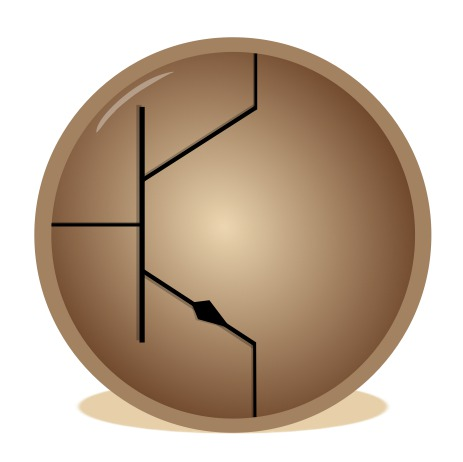
\includegraphics[width=0.3\linewidth]{logo-trimmed.png}
\vfill
\LARGE \textbf{eSim User Manual} \\ 
%\vfill
\small{version 2.0}\\
\vspace{1cm}
\textbf{Prepared By:}\\
eSim Team\\
FOSSEE at IIT, Bombay

\vspace{1cm}

\includegraphics[width=0.2\linewidth]{iitblogo.png} \\
Indian Institute of Technology Bombay \\ [2mm]
{\LARGE \byncnd} \\ [1mm]
March 2020
\end{center}
% \clearpage

% \vfill
% \copyright\ Kannan M. Moudgalya
% \vfill

%\cleardoublepage

%\null\vspace{2.25in}
%\begin{center}
%To \\ [2mm]
%{\large Mr. Narendra Kumar Sinha, IAS \\
%An Electronics Engineer and a Bureaucrat, \\
%Who dreamt of educating all Indians through NMEICT and \\
%Who envisioned and made possible the Aakash Tablet
%}
%\end{center}
%\vfill
\cleardoublepage
 
\newpage

%\pagestyle{empty}
\addtocontents{toc}{\protect\thispagestyle{empty}}
\tableofcontents % adds Index Page

%\pagestyle{empty}

\addtocontents{lof}{\protect\thispagestyle{empty}}

%\listoffigures % adds List of Figures
\cleardoublepage

%\newpage
\cleardoublepage

\section*{Acknowledgement}

There  have  been  many  people contributing towards the software development and/or the electronic system design and simulation for eSim. The following people have contributed in some way.

\subsection*{Development:}
\begin{tasks}[style=itemize](3)
    \task Fahim Khan
    \task Rahul Paknikar
    \task Saurabh Bansode
    \task Gloria Nandihal
    \task Sumanto Kar
    \task Digvijay Singh
    \task Inderjit Dhanjal
    \task Athul George
    \task Gaurav Supal
    \task Kayva Manohar
    \task Komal Sheth


    \task R.V.Rohinth Ram
    \task Madhuri Kadam
    \task Nalinkumar S
    \task Charaan S


    \task Jay Mistry
    \task Manasi Yadav
    \task Bladen Martin
    \task Shubhangi Mahajan
    \task Vadissa Yamini
    \task Ashutosh Jha
    \task Aamir Thekiya

    \task Neel Manilal Shah
    \task Padigepati Mallikarjuna Reddy
    
    \vspace{-1mm}
    
    \task Bhargav Katakam
    \task Anjali Jaiswal
    \task Mahfooz Ahmad

    \task Mudit Joshi
    \task Ashutosh Gangwar
    \task Akshay NH
    \task Athul MS

    
    \task Powai Labs Technology Private Limited
    \task Redwood EDA, LLC
    
    \vspace{-1mm}
    
    \task* VLSI System Design Corporation Ltd.
\end{tasks}


\subsection*{Technical Guidance:}
\begin{multicols}{3}
\begin{itemize}
    \item Kannan Moudgalya
    \item Pramod Murali
    \item Madhav P. Desai
    \item Usha Vishwanathan
    \item Rupak Rokade
    \item Sunil Shetye
\end{itemize}
\end{multicols}

\subsection*{Financial Sponsorship:}
\begin{multicols}{2}
\begin{itemize}
    \item IIT Bombay
    \item NMEICT, MoE, Govt. of India
    
\end{itemize}
\end{multicols}

If someone helped in the development/simulation and has not been inserted in this list, then this omission was unintentional. If you feel you should be on this list, then please feel free to contact us at \href{mailto:contact-esim@fossee.in}{contact-esim@fossee.in}. % Do not be shy, we  would  like  to  make  this  list  as  complete  as possible.
 %adds acknowledgement

\pagenumbering{arabic} %reset numbering to normal for the main content
\chapter{Introduction}
\thispagestyle{empty}
Electronic systems are an integral part of human life. They have
simplified our lives to a great extent. Starting from small systems
made of a few discrete components to the present day integrated
circuits (ICs) with millions of logic gates, electronic systems have
undergone a sea change. As a result, design of electronic systems too
have become extremely difficult and time consuming. Thanks to a host
of computer aided design tools, we have been able to come up with
quick and efficient designs. These are called {\tt Electronic Design
  Automation} or {\tt EDA} \index{EDA! tools}tools.

Let us see the steps involved in EDA.\index{EDA!design flow} In the
first stage, the specifications of the system are laid out. These
specifications are then converted to a design. The design could be in
the form of a circuit schematic, logical description using an HDL
language, etc. The design is then simulated and re-designed, if needed,
to achieve the desired results. Once simulation achieves the
specifications, the design is either converted to a PCB, a chip
layout, or ported to an FPGA. The final product is again tested for
specifications. The whole cycle is repeated until desired results are
obtained %\cite{eda}.

A person who builds an electronic system has to first design the
circuit, produce a virtual representation of it through a schematic
for easy comprehension, simulate it and finally convert it into a
Printed Circuit Board (PCB). \index{PCB} There are various tools
available that will help us do this.  Some of the popular EDA tools 
are those of {\tt Cadence}, {\tt Synopys}, {\tt Mentor Graphics} and 
{\tt Xilinx}. Although these are fairly comprehensive and high end,
their licenses are expensive, being proprietary.

There are some free and open source EDA tools like {\tt gEDA}, {\tt
  KiCad} and {\tt Ngspice}. The main drawback of these open source
tools is that they are not comprehensive. Some of them are capable of
PCB design (e.g. {\tt KiCad}) while some of them are capable of
performing simulations (e.g. {\tt gEDA}).  To the best of our
knowledge, there is no open source software that can perform circuit
design, simulation and layout design together. eSim is capable of
doing all of the above. 

eSim is a free and open source EDA tool.  It is an
acronym for \textbf{E}lectronics \textbf{Sim}ulation. eSim is created 
using open source software packages, such as KiCad, Ngspice and
Python. \index{KiCad} \index{Python} \index{Ngspice}
Using eSim, one can create circuit schematics, perform simulations
and design PCB layouts. It can create or edit new device models, and
create or edit subcircuits for simulation. 

Because of these reasons, eSim is expected to be useful for
students, teachers and other professionals who would want to study
and/or design electronic systems.  eSim is also useful for
entrepreneurs and small scale enterprises who do not have the
capability to invest in heavily priced proprietary tools.

This book introduces eSim to the reader and illustrates all the
features of eSim with examples. The software architecture of eSim is
presented in \chapref{chap2} while \chapref{chap3} gives the user step 
by step instructions to install eSim on a typical computer system. 
\chapref{chap4} gets the user started with eSim. It takes them through 
a tour of eSim with the help of a simple RC circuit example. 
\chapref{chap5} illustrates how to create the circuit schematic in esim 
and \chapref{chap6} explains simulating the circuit schematic. The 
advanced features of eSim such as Model Builder and Sub circuit Builder 
are covered in \chapref{chap7} and \chapref{chap8} respectively. 
Additional features in eSim like mixed mode simulation and 
OpenModelica are covered in \chapref{chap9} and \chapref{chap10} 
respectively. \chapref{chap11} illustrates how to use eSim for solving 
circuit simulation problems. The last chapter, \chapref{chap12} explains 
how eSim can be used to do PCB layout.

The following convention has been adopted throughout this manual.All
the menu names, options under each menu item, tool names, certain
points to be noted, etc., are given in \textit{italics}.  Some
keywords, names of certain windows/dialog boxes, names of some
files/projects/folders, messages displayed during an activity, names
of websites, component references, etc., are given in {\tt typewriter}
font. Some key presses, e.g. {\tt Enter} key, {\tt F1} key, {\tt y}
for yes, etc., are also mentioned in {\tt typewriter} font.
 % adds the chapter 1 introduction

\chapter {Architecture of eSim}
\thispagestyle{empty}
\label{chap2}

eSim is a CAD \index{CAD} tool that helps electronic system designers
to design, test and analyse their circuits. But the important feature
of this tool is that it is open source and hence the user can modify
the source as per his/her need. The software provides a generic,
modular and extensible platform for experiment with electronic
circuits. This software runs on Ubuntu Linux LTS distributions 18.04 and 20.04, and  Microsoft Windows 7, 8 and 10.
It uses {\tt Python 3}, {\tt KiCad 4.0.7}, {\tt Makerchip},
{\tt GHDL}, {\tt Verilator} and {\tt Ngspice}.

The objective behind the development of eSim is to provide an open
source EDA solution for electronics and electrical engineers. The 
software should be capable of performing schematic creation, PCB 
design and circuit simulation (analog, digital and mixed-signal). 
It should provide facilities to create new models and components. 
The architecture of eSim has been designed by keeping these 
objectives in mind. 

\section {Modules used in eSim}
Various open-source tools have been used for the underlying build-up 
of eSim. In this section we will give a brief idea about all the modules 
used in eSim. 

\subsection {Eeschema} \index{Eeschema} \index{KiCad}
Eeschema is an integrated software where all functions of circuit
drawing, control, layout, library management and access to the PCB
design software are carried out.  It is the schematic
editor tool used in KiCad. %\cite{eeschema}. 
Eeschema is intended to
work with PCB layout software such as Pcbnew. It provides netlist that
describes the electrical connections of the PCB. Eeschema also
integrates a component editor which allows the creation, editing and
visualization of components. It also allows the user to effectively
handle the symbol libraries i.e; import, export, addition and deletion
of library components.  Eeschema also integrates the following
additional but essential functions needed for a modern schematic
capture software:

\begin{inparaenum}
\item Design rules check \index{Design rules check} ({\tt DRC}) for 
the automatic control of incorrect connections and inputs of components 
left unconnected.
\item Generation of layout files in {\tt POSTSCRIPT} \index{POSTSCRIPT}or 
{\tt HPGL} \index{HPGL} format.
\item Generation of layout files printable via printer.
\item Bill of materials generation.
\item Netlist generation for PCB layout or for simulation.
\end{inparaenum}

This module is indicated by the label 1 in \figref{blockd}.

As Eeschema is originally intended for PCB Design, there are no
fictitious components\footnote{Signal generator or power supply is not
  a single component but in circuit simulation, we consider them as a
  component.  While working with actual circuit, signal generator or
  power supply gives input to the circuit externally thus, doesn't
  require for PCB design.} such as voltage or current sources. Thus,
we have added a new library for different types of voltage and current
sources such as sine, pulse and square wave.  We have also built a
library which gives printing and plotting solutions.
This extension, developed by us for eSim, is indicated by the label
2 in \figref{blockd}.

\subsection {CvPcb}
\index{CvPcb} CvPcb is a tool that allows the user to associate
components in the schematic to component footprints when designing the
printed circuit board. CvPcb is the footprint editor tool in KiCad.
%\cite{eeschema}. 
Typically the netlist file generated by Eeschema does
not specify which printed circuit board footprint is associated with
each component in the schematic. However, this is not always the case
as component footprints can be associated during schematic capture by
setting the component's footprint field. CvPcb provides a convenient
method of associating footprints to components. It provides footprint
list filtering, footprint viewing, and 3D component model viewing to
help ensure that the correct footprint is associated with each
component. Components can be assigned to their corresponding
footprints manually or automatically by creating equivalence
files. Equivalence files are look up tables associating each component
with its footprint. This interactive approach is simpler and less
error prone than directly associating footprints in the schematic
editor.  This is because CvPcb not only allows automatic association,
but also allows to see the list of available footprints and displays
them on the screen to ensure the correct footprint is being
associated.  This module is indicated by the label 3 in
\figref{blockd}.  

\subsection {Pcbnew}
\index{Pcbnew} Pcbnew is a powerful printed circuit board software
tool. It is the layout editor tool used in KiCad. %\cite{eeschema}. 
It
is used in association with the schematic capture software Eeschema,
which provides the netlist. Netlist describes the electrical
connections of the circuit. CvPcb is used to assign each component, in
the netlist produced by Eeschema, to a module that is used by
Pcbnew. The features of Pcbnew are given below:
\begin{itemize}
\item It manages libraries of modules. Each module is a drawing of the
  physical component including its footprint\index{Footprints} - the
  layout of pads providing connections to the component. The required
  modules are automatically loaded during the reading of the netlist
  produced by CvPcb.
\item Pcbnew integrates automatically and immediately any circuit
  modification by removal of any erroneous tracks, addition of 
  new components, or by modifying any value (and under certain
  conditions any reference) of old or new modules, according to
  the electrical connections appearing in the schematic.   
\item This tool provides a rats nest display, a hairline connecting
  the pads of modules connected on the schematic. These
  connections move dynamically as track and module movements are
  made. 
\item It has an active Design Rules Check ({\tt DRC}) which
  automatically indicates any error of track layout in real time. 
\item It automatically generates a copper plane, with or without
  thermal breaks on the pads.  
\item It has a simple but effective auto router to assist in the
  production of the circuit. An export/import in {\tt SPECCTRA}
  dsn format allows to use more advanced
  auto-routers.  
\item It provides options specifically for the production of ultra
  high frequency circuits (such as pads of trapezoidal and complex
  form, automatic layout of coils on the printed circuit).  
\item Pcbnew displays the elements (tracks, pads, texts, drawings and
  more) as actual size and according to personal preferences such as: 
\begin{itemize}
\item display in full or outline.
\item display the track/pad clearance.
\end{itemize}
\end{itemize}
This module is indicated by the label 4 in
\figref{blockd}.
\subsection{KiCad to Ngspice converter}
Analysis parameters, and the source details are provided through this module. It also allows us to add and edit the device models and subcircuits, included in the circuit schematic.  Finally, this module facilitates the conversion of KiCad netlist to Ngspice compatible ones. 
\\
It is developed by us for eSim and it is indicated by the label 7 in \figref{blockd}. The use of this module is explained in detail in section (yet to be put).

%Commenting and putting it in next chapter

%\subsubsection{Analysis Inserter}
%This feature helps the user to perform different types of analysis such
%as Operating point analysis, \index{Operating point analysis} DC
%analysis, \index{DC Analysis} AC analysis, \index{AC Small-signal
%Analysis} transient analysis, \index{Transient Analysis}. It has
%the facility to
%\begin{itemize}
%\item Insert type of analysis such as AC or DC or Transient
%\item Insert values for analysis
%\end{itemize}
%\subsubsection {Source Details}
%eSim sources are added from eSim-sources package. Sources auch as \textit{SINE, AC, DC, PULSE} are in this library. The parameter values to all the sources added in the schematic can be given through 'Source Details'.
%\subsubsection {Ngspice Model}
%Ngspice has in built model such as \textit{flipflop(D,SR,JK,T),gain,summer} etc. which can be utilised while building a circuit.
%eSim allows to add and modify Ngspice model parameter through Ngspice Model tab.
%\subsubsection {Device Modeling}
%Devices like \textit{Diode, JFET, MOSFET, IGBT, MOS} etc added in the circuit can be modeled using device model libraries. eSim also provides editing and adding new model libraries. While converting Kicad to Ngspice these library files are added to the corresponding devices used in the circuit.
%\subsubsection {Subcircuits}
%Subcircuits are the circuits within a circuits. Subcircuiting helps to reuse the part of the circuits.
%The sub circuit in the main circuits are added using this facility. Also, eSim provides us with editing the already existing subcircuits.
%%
\subsection {Model Builder} \index{Model Builder}
This tool provides the facility to define a new model for devices such
as,
\begin{inparaenum}
            \item Diode
            \item Bipolar Junction Transistor (BJT)
            \item Metal Oxide Semiconductor Field Effect Transistor (MOSFET)
            \item Junction Field Effect Transistor (JFET)
            \item IGBT and
            \item Magnetic core.
            \end{inparaenum}
            This module also helps edit existing models.
It is developed by us for eSim and it is indicated by the
label 5 in \figref{blockd}.
 
\subsection{Subcircuit Builder} \index{Subcircuit Builder} This
module allows the user to create a subcircuit for a component. Once
the subcircuit for a component is created, the user can use it in
other circuits. It has the facility to define new components such as,
Op-amps, IC-555, UJT and so on.  This component also helps edit existing
subcircuits.  This module is developed by us for eSim and it is
indicated by the label 6 in \figref{blockd}.

\subsection{Ngspice} \index{Ngspice} \label{sec:ngspice}
Ngspice is a general purpose circuit simulation program for nonlinear
dc, nonlinear transient, and linear ac analysis.
%\cite{ngspice-web}. 
Circuits may contain resistors, capacitors,
inductors, mutual inductors, independent voltage and current sources,
four types of dependent sources, lossless and lossy transmission lines
(two separate implementations), switches, uniform distributed RC
lines, and the five most common semiconductor devices: diodes,
\index{diode} BJTs, \index{BJT} JFETs, MESFETs,
and MOSFET. \index{MOSFET}
This module is indicated by the label 9 in \figref{blockd}.

\subsection{NGHDL} \index{NGHDL} \label{sec:nghdl}
NGHDL, a module for mixed signal circuit simulation, is also integrated with eSim.  It makes use of VHDL code.
It uses ghdl for digital simulation and the mixed signal simulation happens through 
Ngspice.

\subsection{NgVeri} \index{NgVeri} \label{sec:NgVeri}
NgVeri, a module for mixed signal circuit simulation, is also integrated with eSim. It makes use of Verilog/System Verilog/Transaction-Level Verilog  code.
It uses SandPiper SaaS and Verilator for digital simulation and the mixed signal simulation happens through 
Ngspice. 

\subsection{Makerchip-App} \index{Makerchip-App} \label{sec:Makerchip-App}
Makerchip is a cloud based browser application developed by Redwood EDA to do digital circuit design. One can simulate Verilog/SystemVerilog/Transaction-Level Verilog code in Makerchip. eSim is interfaced with Makerchip using a Python based application called Makerchip-App which launches the Makerchip IDE.

\subsection{SandPiper SaaS} \index{SandPiper SaaS} \label{sec:Sandpiper-saas}
Sandpiper-saas is a tool developed by Redwood EDA which converts Transaction Level Verilog code to SystemVerilog code. It is used by NgVeri so that it can get the System Verilog code which can be further passed to the Verilator.

\subsection{Verilator} \index{Verilator} \label{sec:Verilator}
Verilator is a Verilog/SystemVerilog simulator tool. It converts the Verilog/SystemVerilog code to C++ object files. These object files are linked with that of Ngspice thus enabling mixed signal simulation in eSim.

\subsection{OpenModelica} \index{OpenModelica} \label{sec:openmodelica}
OpenModelica (OM) is an open source modeling and simulation tool based on
Modelica language. Two modules of OpenModelica, OMEdit, an IDE for modeling 
and simulation and OMOptim, an IDE for optimisation are integrated with eSim.

\section {Work flow of eSim}

\begin{figure}
\centering
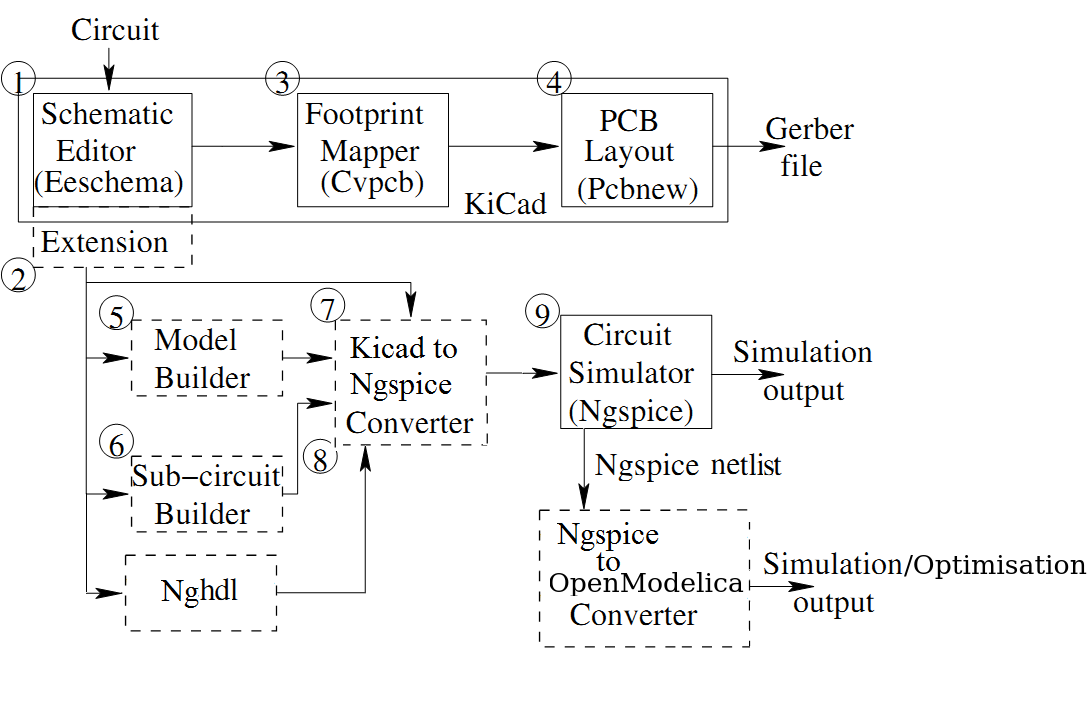
\includegraphics[width=\hgfig]
{blockdiagram.png}
\caption{Work flow in eSim. (Boxes with dotted lines denote
  the modules developed in this work).}
%\caption{Workflow of Oscad}
\label{blockd}
\end{figure}

\figref{blockd} shows the work flow in eSim. The block diagram consists of mainly three parts: 
\begin{itemize}
\item Schematic Editor 
\item PCB Layout Editor  
\item Circuit Simulators
\end{itemize} 



%
Here we explain the role of each block in designing electronic
systems. Circuit design is the first step in the design of an electronic
circuit. Generally a circuit diagram is drawn on a paper, and then
entered into a computer using a schematic editor. Eeschema is the
schematic editor for eSim. Thus all the functionalities of Eeschema
are naturally available in eSim.  \index{EEschema}

Libraries for
components, explicitly or implicitly supported by Ngspice, have been
created using the features of Eeschema. As Eeschema is originally intended for PCB design, there are
no fictitious components such as voltage or current sources. Thus, a
new library for different types of voltage and current sources such as
sine, pulse and square wave, has been added in eSim. A library
which gives the functionality of printing and plotting has also been
created. 

The schematic editor provides a netlist file, which describes the
electrical connections of the  design. In order to create a PCB
layout, physical components are required to be mapped into their
footprints. To perform component to footprint mapping, CvPcb  is
used. Footprints have been created for the
components in the newly created libraries. Pcbnew is used to draw a
PCB layout. 

After designing a circuit, it is essential to check the integrity of
the circuit design. In the case of large electronic circuits,
breadboard testing is impractical. In such cases, electronic system
designers rely heavily on simulation. 
The accuracy of the simulation results can be increased by accurate
modeling of the circuit elements.
Model Builder provides the facility
to define a new model for devices and edit existing models. Complex
circuit elements can be created by hierarchical modeling. Subcircuit
Builder provides an easy way to create a subcircuit. 

The netlist generated by Schematic Editor cannot be directly used
for simulation due to compatibility issues. Netlist Converter converts
it into Ngspice compatible format. The type of simulation
to be performed and the corresponding options are
provided through a graphical user interface (GUI). This is called
KiCad to Ngspice Converter in eSim. 

eSim uses Ngspice for analog, digital, mixed-level/mixed-signal circuit
simulation. Ngspice is based on three open source software
packages%\cite{spice}:  
\begin{itemize}
\item Spice3f5 (analog circuit simulator) 
\item Cider1b1 (couples Spice3f5 circuit simulator to DSIM device simulator)
\item Xspice (code modeling support and simulation of digital components through an event driven algorithm)
\end{itemize}
It is a part of gEDA \index{gEDA} project. Ngspice is capable of
simulating devices with BSIM, \index{BSIM} EKV,  HICUM, \index{EKV}
\index{HICUM} HiSim, \index{HiSim} PSP, \index{PSP} and PTM \index{PTM}
models. It is widely used due to its accuracy even for the latest
technology devices.
 % adds chapter 2
\chapter{Installing eSim}
\thispagestyle{empty}
\label{chap3}

\section {eSim installation in Ubuntu OS}
\begin{enumerate}
\item Download eSim installer for Linux from {\tt http://esim.fossee.in/downloads} to a local directory and unpack it. You can also unpack the  installer through the terminal. Open the terminal and navigate to the directory where this INSTALL file is located. Use the following command to unpack:
\\
\quad {\tt \$ unzip eSim-2.1.zip}
\item To install eSim and other dependencies run the following command:
\\
 \quad {\tt \$ cd eSim-2.1 \newline \$ chmod +x install-eSim.sh \newline \$ ./install-eSim.sh --install}
\item To run eSim from the terminal, type:  
\\
\quad {\tt \$ esim}
\\
  or you can double click on {\tt eSim} icon created on the Desktop after installation.
\end{enumerate}


\section {eSim installation in Windows OS}
\begin{enumerate}
\item Download \textbf{eSim-2.1\_install.exe} from  {\tt https://esim.fossee.in/downloads}
\item Disable the antivirus (if any). Now, double click on the exe file to start the installation process. If a window appears, click {\tt Yes} to complete the installation.
\item By default eSim will be installed in C drive, under an auto-generated FOSSEE Folder. Note that installation directory can neither be in "Program Files" nor contain spaces in its path.
\item \textbf{eSim} icon will be created on desktop. You can double click on the {\tt eSim} icon created on the Desktop after installation.
\end{enumerate}

% adds chapter 3
%\usepackage{appendix}
\chapter {Getting Started}
\thispagestyle{empty}
\label{chap4}

In this chapter we will get started with eSim. Referring to
this chapter will make one familiar with eSim and will help
plan the project before actually designing a circuit. 

\section{How to launch eSim?}
After the installation of eSim, a shortcut to eSim is created 
on the Desktop. To launch eSim double click on the shortcut.\\ 
Alternately, for Ubuntu Linux users, one can also launch eSim from the terminal.\\
1. Go to terminal.\\
2. Type \textbf{esim} and press {\tt Enter}.\\

The first window that appears is the workspace dialog as shown in 
\figref{workspace}. 
\begin{figure}[h]
\centering
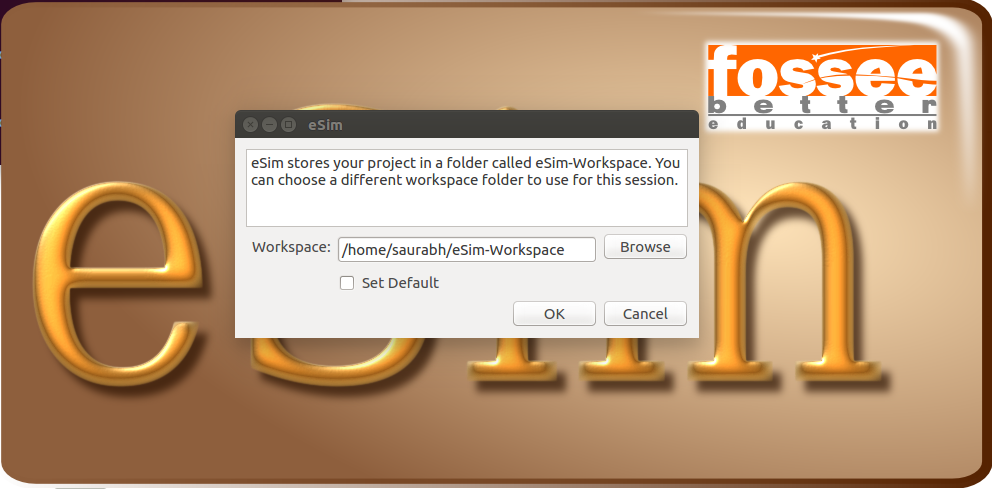
\includegraphics[width=\lgfig]{workspace.png} 
\caption{eSim-Workspace}
\label{workspace}
\end{figure}

\item 1.The default workspace is eSim-Workspace under home directory. 
To select a new workspace location, use the {\tt browse} option. Do not select a location which has a space character or special character(s). 
\item 2. If you select the \textbf{set default} click-box, then the chosen location will be set as default workspace and the dialog box won't appear next time you launch eSim.
\item 3. If you wish to change the default workspace location, then use the menu-bar from eSim's main Interface, which is explained in upcoming section.
\section{eSim User Interface}
The main graphic window of eSim is as shown in \figref{maingui}.
\begin{figure}[h]
\centering
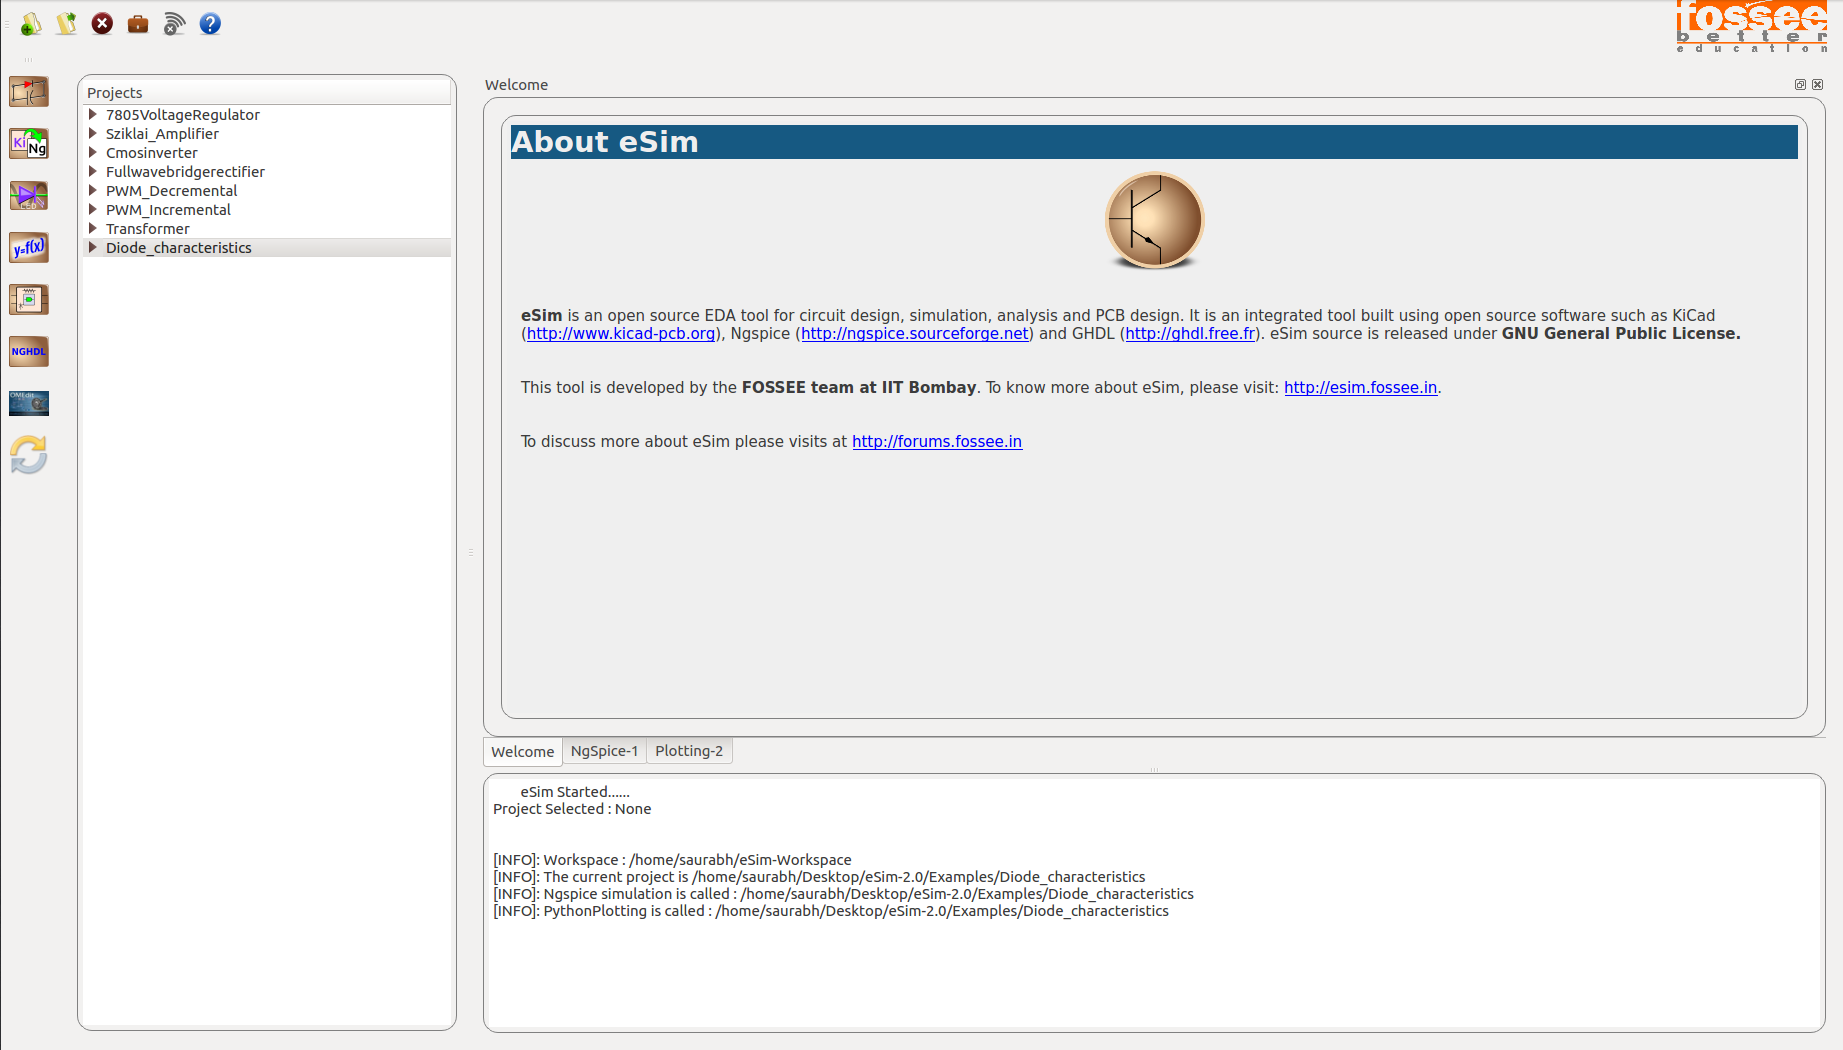
\includegraphics[width=\hgfig]{maingui.png}
\caption{eSim Main GUI}
\label{maingui}
\end{figure}
\\
The eSim window consists of the following sections.
\begin{enumerate}

\item Menubar
\item Toolbar
\item Project explorer
\item Dockarea
\item Console area
\end{enumerate}

\subsection{Menubar}
\begin{itemize}
\item \textbf{New Project}:
New projects are created in the eSim-Workspace. When this menu is selected, 
a new window opens up with {\tt Enter Project name} field. Type the name of 
the new project and click on {\tt OK}. A project directory will be created in 
eSim-Workspace. The name of this folder will be the same as that of the 
project created. \textit {Make sure that the project name does not have 
any spaces in between.} This project is also added to the project explorer.

\item \textbf{Open Project}:
This opens the file dialog of default eSim-Workspace where the projects are stored. 
Select the required project and click on {\tt Open}. The selected project is added 
to the project explorer.

\item \textbf{Close Project}:
This button closes the opened project.

\item \textbf{Change workspace} : Clicking on this will open the window shown in \figref{workspace}. If you have chosen a default workspace location but wish to change it later on, launch eSim, click on this icon and do the necessary changes. 

\item \textbf{Mode Switch} : Using this feature user can decide whether to fetch latest footprints(refer Section :PCB Designing) from the internet or use the locally available footprints. \\
Note : By switching to online mode, you will require a stable and high-speed internet connection, if it is not available to you then please always remain in the offline mode.

\item \textbf{Help} : Clicking on this icon will launch the eSim user manual for that particular version of eSim. 
\end{itemize}

\subsection{Toolbar}
The toolbar consists of the following buttons. See \figref{guitoolbar}.

\begin{figure}[h]
\centering
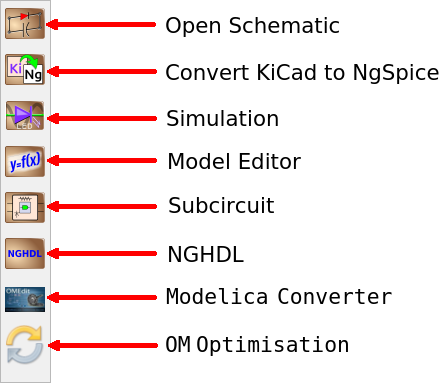
\includegraphics[width=\lgfig]{manual_images/guitoolbar.PNG}
\caption{Toolbar}
\label{guitoolbar}
\end{figure}

\subsubsection {Open Schematic}
The first button on the toolbar is the \texttt{Schematic
Editor}\index{Schematic!editor}. Clicking on this button 
will open the schematic editor. 
If  a new project  is  being  created, one will get a 
dialog box confirming the creation of a schematic. This 
is illustrated in See \figref{schematic-confirmation}. 
However, if an already existing project is opened, the 
schematic editor window is opened. To know how to use 
the schematic editor to create circuit schematics, refer 
to \chapref{chap5}. \\ \\
When one right clicks on a particular project : three options appear, their functions listed below: \\
\begin{enumerate}
    \item Rename Project : This will rename the project and the underlying files. Note that all project files must be closed from all running applications that access them before renaming a project.
    \item Remove Project : This will remove the project selected from the \texttt{Project Explorer} list.
    \item Refresh : At times, all the files under a project will not be displayed. In that case, selecting this option will update the latest files under a project. 
\end{enumerate}
\begin{figure}[h]
\centering
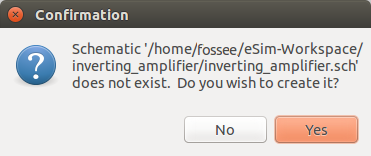
\includegraphics[width=\lgfig]{manual_images/schematic-confirmation.png}
\caption{Confirmation for schematic creation}
\label{schematic-confirmation}
\end{figure}

\subsubsection {Convert KiCad to Ngspice}
In the schematic editor window, after creating the schematic a netlist is to be  generated which contains information about the components present in the schematic created and their values specified . Although this netlist is present, it cannot be directly fed to the simulator. Here the KiCad-to-Ngspice converter comes into play.
This tool converts the netlist generated from the schematic into another netlist which is compatible with Ngspice, the simulator used in eSim.
The \textbf{Convert KiCad to Ngspice} window consists of five tabs namely \texttt{Analysis, Source Details, Ngspice Model, Device Modeling and Subcircuits}.
The details of these tabs are as follows.\\
\begin{itemize}
\item \texttt{Analysis:} This feature helps the user to enter the parameters for performing different types of analysis such as Operating point analysis, \index{Operating point analysis} DC analysis, \index{DC Analysis} AC analysis, \index{AC Small-signal Analysis} transient analysis, \index{Transient Analysis} DC Sweep Analysis. \index{DC Sweep Analysis}

It has the facility to select the
\begin{itemize}
    \item Type of analysis and
    \item The simulation parameter values for analysis
\end{itemize}

\item \texttt{Source Details:}eSim sources are added from {\tt eSim\_Sources} library in the \linebreak schematic. Sources such as \textit{SINE, AC, DC, PULSE, PWL} are in this library. The parameter values to all the sources added in the schematic can 
be given through 'Source Details' tab in the KiCad-To-Ngspice window.

\item \texttt{Ngspice Model:}Ngspice has in-built model such as \texttt{basic logic gates, \linebreak flip-flops, gain, summer, buffer, DAC and ADC block}etc. which can be utilised while building a circuit.
eSim allows to add and modify Ngspice model parameter through 
Ngspice Model tab.

\item \texttt{Device Modeling:}Devices like \texttt{Diode, JFET, MOSFET, IGBT, MOS} etc used in 
the circuit can be modeled using device model libraries. eSim also 
provides editing and adding new model libraries. While converting 
KiCad to Ngspice, these library files are added to the corresponding 
devices used in the circuit.

\item \texttt{Subcircuits:}eSim allows you to build subcircuits.  The subcircuits can again 
have components having subcircuits and so on. This enables users to 
build commonly used circuits as subcircuits and then use it across 
circuits. The subcircuits are added to the main circuits using this 
facility. We can also edit already existing subcircuits. 
\\
Once the values have been entered, press the {\tt Convert} button. This 
will generate the {\tt .cir.out} file in the same project directory.
Note that \textit{KiCad to Ngspice Converter} can only be used if 
the KiCad spice netlist {\tt .cir} file is already generated.
\\
\end{itemize}

\subsubsection {Simulation}
The netlist generated using the \texttt{KiCad to Ngspice} converter 
is simulated using \textit{Simulation} button on the eSim left toolbar. This
will run the Ngspice simulation for current project. eSim have two options 
to see the simulation output. The first one is the Python plotting window 
which opens up in the dock area, as shown in \figref{simulation-op}. 
The second is the Ngspice window with the simulation data. The user can 
type in Ngspice commands to view the plots. 

\textit {Note: If the user has used the plot components (available under eSim\_Plot library) at various nodes in the circuit schematic the Ngspice plots are displayed automatically.}

\begin{figure}[h]
\centering
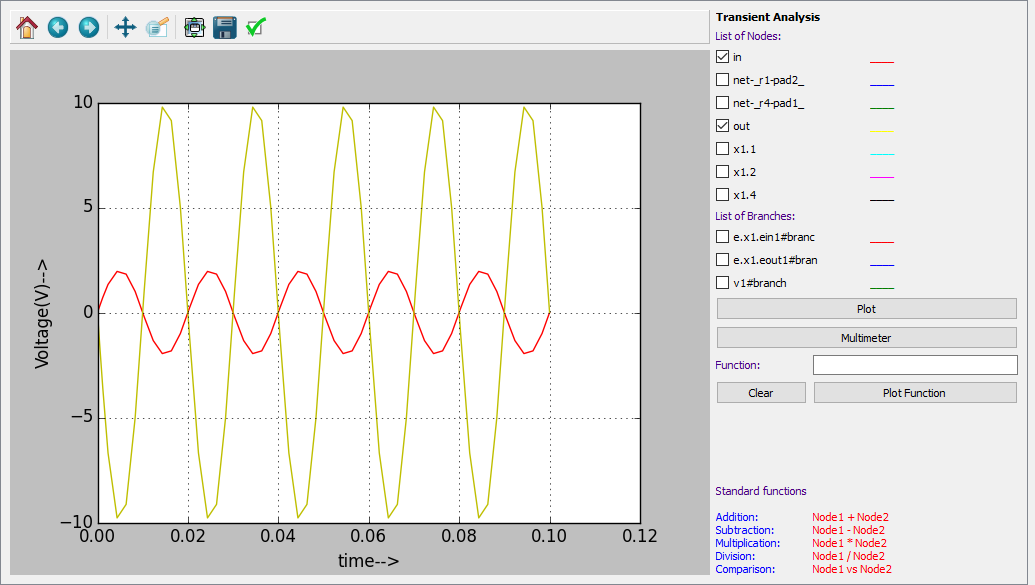
\includegraphics[width=\hgfig]{manual_images/simulation-op.png}
\caption{Simulation Output in Python Plotting Window}
\label{simulation-op}
\end{figure}

%\subsubsection {Foot Print Editor:}
%Clicking on the \textit{Footprint Editor} tool will open the {\tt CvPcb} 
%\index{CvPcb} window. This window will ideally open the .net file for the 
%current project. So, before using this tool, one should have the netlist 
%for PCB design (a .net file). %To know more about how to assign footprints 
%to components, see \chapref{chap7}.

%\subsubsection {PCB Layout:}
%Clicking on the \textit{Layout Editor} tool will open {\tt
%Pcbnew}\index{Pcbnew}, the layout editor used in eSim. In this
%window, one will create the PCB. It involves laying tracks and vias,
%performing optimum routing of tracks, creating one or more copper
%layers for PCB, etc. It will be saved as a {\tt .brd} file in the 
%current project directory. %\chapref{chap7} explains how to use the 
%\textit{Layout Editor} to design a PCB. 

\subsubsection {Model Editor}
eSim also gives an option to re-configure the model library of a
device. It facilitates the user to change model library of devices
such as diode, transistor, MOSFET, etc. It also facilitates the user to load the spice library externally and use it for the existing or newly added models.To know
more about Model Editor, refer to \chapref{chap7}.

\subsubsection {Subcircuit}
eSim also allows the user to build subcircuits. The subcircuits can
again have components having subcircuits and so on. This enables users
to build commonly used circuits as subcircuits and then use it across
circuits. For example, one can build an Op-Amp as a
subcircuit and then use it as just a single component across circuits
without having to recreate it. Clicking on \textit{Subcircuit
Builder} tool will allow one to edit or create a subcircuit. To know
how to make a subcircuit, refer to \chapref{chap8}.

\subsubsection {NGHDL}
NGHDL is an add on to eSim for mixed signal circuit simulation. By using the foreign language interface of GHDL, NGHDL communicates with Ngspice and accomplishes mixed signal simulation. Using NGHDL, user can create custom digital model using VHDL language. From simple multiplexers, counters to microcontrollers and ASICs, any custom component in the digital domain can be realized using the NGHDL tool. The created digital model can be used in either mixed signal circuit or a standalone circuit operating in digital domain. NGHDL gives user the liberty to edit existing models supplied with eSim per their needs, either for experimenting new ideas or to change the model per their specific requirement.

\subsubsection {Modelica Converter}
OpenModelica (OM) is an open source modeling and simulation tool based on
Modelica language. Modelica is an object oriented language. The Modelica Converter in eSim interface, converts the ngspice netlist to Modelica format. This facility will be only available if you have OpenModelica already installed in the system. More details on how to use this module is available in \chapref{chap10}.

\subsubsection {OM Optimisation}
OMOptimisation (OMOptim) is a powerful and interactive tool for performing design optimisation. It has a good library of electrical components called Modelica Standard Library (MSL). OMOptim is stable and robust. It is very easy to add objective functions to the OMOptim interface.

\subsection{Project Explorer}
Project explorer contains the list of all the projects previously added to it. 
Select a project and double click on it, this will display all the files under 
this project. Right click on any displayed file to open it. To remove or refresh 
any project file from the project explorer, right click on the main project file.


\subsection{Dockarea}
This area is used to open the following windows.
\begin{enumerate}
    \item KiCad to Ngspice converter
    \item Ngspice plotting
    \item Python plotting
    \item Model builder
    \item Subcircuit builder
\end{enumerate}
Modules/Windows will appear here as per your selection.

\subsection{Console Area}
Console area provides the log information about the activity done during the current session.


 % adds chapter 4
%\documentclass[12pt]{report}
%\usepackage{amsmath,graphicx,makeidx}

%\makeindex
%\begin{document}
%\tableofcontents

\chapter{Schematic Creation}
\thispagestyle{empty}
\label{chap5}
The first step in the design of an electronic system is the design of
its circuit. This circuit is usually created using a {\tt Schematic
  Editor}\index{Schematic!editor} and is called a {\tt
  Schematic}. \index{Schematic} eSim uses {\tt Eeschema}
\index{Eeschema} as its schematic editor. Eeschema is the schematic
editor of KiCad.  \index{KiCad} It is a powerful schematic editor
software. It allows the creation and modification of components and
symbol libraries and supports multiple hierarchical layers of printed
circuit design.

\section{Familiarizing the Schematic Editor interface}
\figref{eesch1} shows the schematic editor and the various menu and
toolbars.  We will explain them briefly in this section.
\begin{figure}[h]
\begin{center}
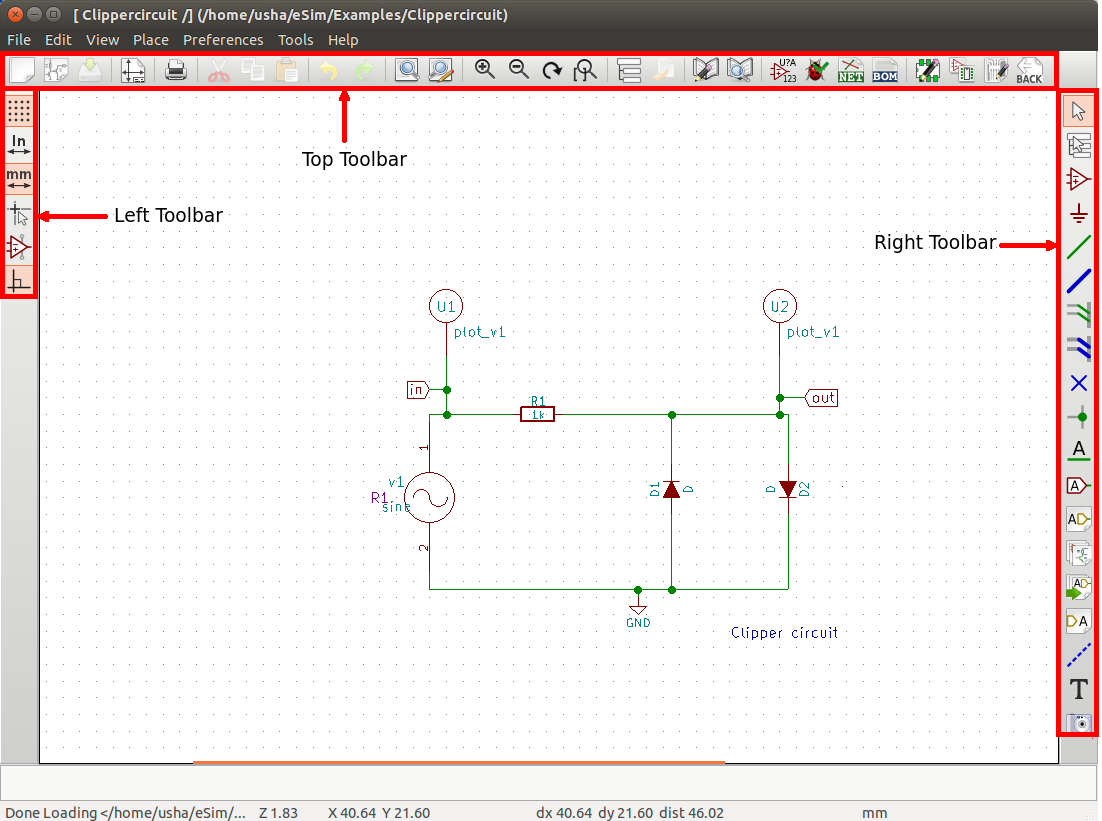
\includegraphics[width=\linewidth]{manual_images/schematic1.png}
%If the fig is appearing too big/small, change the scaling factor 0.2
\caption{Schematic editor with the menu bar and toolbars marked}
\label{eesch1}
\end{center}
\end{figure}

\subsection{Top menu bar}
The top menu bar will be available at the top left corner.
Some of the important menu options in the top menu bar are:

\begin{compactenum}
\item File - 
The file menu items are given below:
\begin{compactenum}
\item New - Clear current schematic and start a new one
\item Open - Open a schematic 
\item Open Recent - A list of recently opened files for loading
\item Save Schematic project - Save current sheet and all its
  hierarchy.
\item Save Current Sheet Only - Save current sheet, but not others in
  a hierarchy.
\item Save Current sheet as - Save current sheet with a new name.
\item Page Settings - Set preferences for printing the page.
\item Print - Access to print menu (See \figref{print}).
\item Plot - Plot the schematic in Postscript, HPGL, SVF or DXF format 
\item Close - Close the schematic editor. 
\end{compactenum}
\begin{figure}[h]
\begin{center}
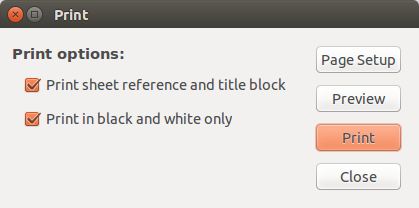
\includegraphics[width=0.5\linewidth]{manual_images/print.png}
\caption{Print options}
\label{print}
\end{center}
\end{figure}

\item Place - 
The place menu has shortcuts for placing various items like
components, wire and junction, on to the schematic editor window. See
\secref{short} to know more about various shortcut keys (hotkeys). 

\item Preferences - 
The preferences menu has the following options:
\begin{compactenum}
\item Component Libraries - Select component libraries and library paths. This enables the user to add the libraries, if the libraries are not loaded in the Eeschema.
\item Schematic Editor Options - Select colors for various items, display 
options and set hot keys.
\item Language - Shows the current list of available languages. Use default. 
\item Import and Export - Contain options to load and save preferences and 
import/ export hot key configuration files. See \secref{short} to know about 
various hotkeys.
\end{compactenum}

\end{compactenum} 

\subsection{Top toolbar}\index{Schematic!toolbar!top}\index{Eeschema!toolbar!top}
Some of the important tools in the top toolbar are discussed
below. They are marked in \figref{eeschem2}.
\begin{figure}[h]
\centering
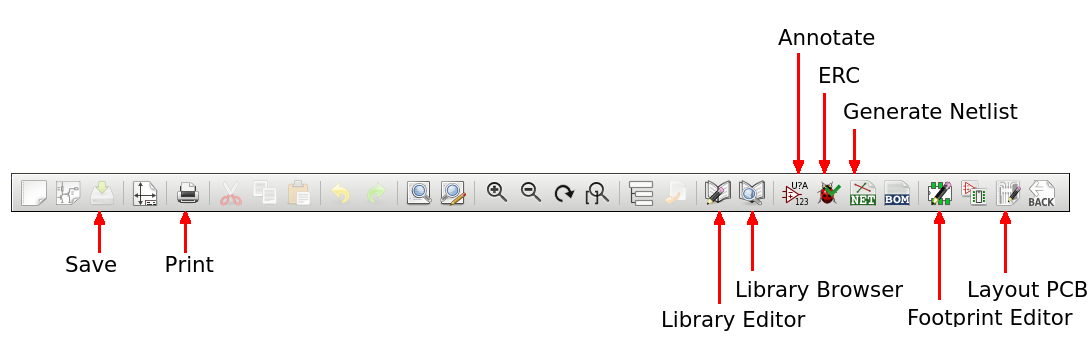
\includegraphics[width=\textwidth]{manual_images/toptoolbar.png}
\caption{Toolbar on top with important tools marked}
\label{eeschem2}
\end{figure}
\begin{compactenum}
\item Save - Save the current schematic
\item Print - Print the schematic
\item Navigate schematic hierarchy - Navigate among the root and
  sub-sheets in the hierarchy
\item Library Editor - Create or edit components.
\item Library Browser - Browse through the various component libraries
  available
\item Annotate - Annotate the schematic
\item Check ERC - Do Electric Rules Check for the schematic
\item Generate Netlist - Generate a netlist for PCB design({\tt .net}) or for
  simulation({\tt .cir}).
\item Create BOM - Create a Bill of Materials of the schematic
\item Footprint editor - Map each component in the PCB netlist to a footprint
\item Layout PCB - Lay tracks between the footprints to get the PCB layout
\end{compactenum}

\subsection{Toolbar on the right}\index{Schematic!toolbar!right}\index{Eeschema!toolbar!right}
The toolbar on the right side of the schematic editor window has many
important tools. Some of them are marked in \figref{eeschem3}.
\begin{figure}[h]
\centering
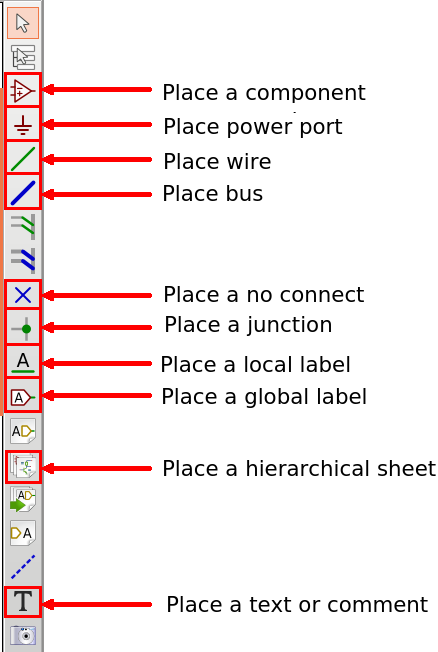
\includegraphics[width=7cm,height=10cm]{manual_images/righttoolbar.png}
\caption{Toolbar on right with important tools marked}
\label{eeschem3}
\end{figure}
Let us now look at each of these tools and their uses.
\begin{compactenum}
\item Place a component - Load a component to the schematic. See
  \secref{selplace} for more details.
\item Place a power port - Load a power port (Vcc, ground) to the schematic.
\item Place wire - Draw wires to connect components in schematic.
\item Place bus - Place a bus on the schematic.
\item Place a no connect - Place a no connect flag, particularly useful in ICs.
\item Place a local label - Place a label or node name which is local to the schematic.
\item Place a global label - Place a global label (these are connected across all schematic diagrams in the hierarchy).
\item Create a hierarchical sheet - Create a sub-sheet within the root sheet in the hierarchy. Hierarchical schematics is a good solution for big projects.
\item Place a text or comment - Place a text or comment in the schematic.
\end{compactenum}
\subsection{Toolbar on the left}\index{Schematic!toolbar!left}\index{Eeschema!toolbar!left}
Some of the important tools in the toolbar on the left are discussed
below. They are marked in \figref{eeschem4}.
\begin{figure}[h]
\centering
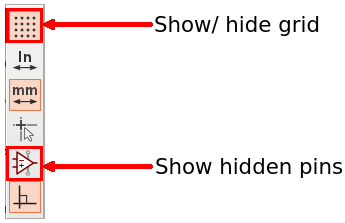
\includegraphics[width=0.4\textwidth]{manual_images/lefttoolbar.png}
\caption{Toolbar on left with important tools marked}
\label{eeschem4}
\end{figure}

\begin{compactenum}
\item Show/Hide grid - Show or Hide the grid in the schematic editor. Pressing the tool again hides (shows) the grid if it was shown (hidden) earlier.
\item Show hidden pins - Show hidden pins of certain components, for  example, power pins of certain ICs. 
\end{compactenum}

\subsection{Hotkeys}
\label{short}
A set of keyboard keys are associated with various operations in the
schematic editor. These keys save time and make it easy to switch from
one operation to another. The list of hotkeys can be viewed by going
to Preferences in the top menu bar. Choose \textit{Schematic Editor Options} and select \textit{Controls} tab. The hotkeys can also be edited here. Some frequently used hotkeys, along with their functions, are given below:
\begin{compactitem}
\item F1 - Zoom in
\item F2 - Zoom out
\item Ctrl + Z - Undo
\item Delete - Delete item
\item M - Move item
\item C - Copy item
\item A - Add/place component 
\item P - Place power component
\item R - Rotate item
\item X - Mirror component about X axis
\item Y - Mirror component about Y axis
\item E - Edit schematic component
\item W - Place wire
\item T - Add text
\item S - Add sheet
\end{compactitem}
\textit{Note: Both lower and upper-case keys will work as hotkeys}. 

\section{eSim component libraries}% \index{Schematic!for
  %simulation} 

eSim schematic editor has a huge collection of components. As Eeschema is  meant  to  be  a  schematic  editor  to  create  circuits  for  PCB,  Eeschema  lacks  some components that are necessary for simulation (e.g.  probes(plot\_v and current sources). A set of component libraries has been created with such components under the label \textit{eSim\_*}. These libraries are Ngspice compatible.  If one is using eSim only  for  designing  a  PCB,  then  one  might  not  need  these  libraries. However, these libraries are essential if one needs to simulate one's circuit. Hereafter, we will refer to these libraries as eSim libraries to distinguish them from libraries already present in Eeschema (Eeschema libraries) as shown in \figref{libraries}.
\begin{figure}[h]
\centering
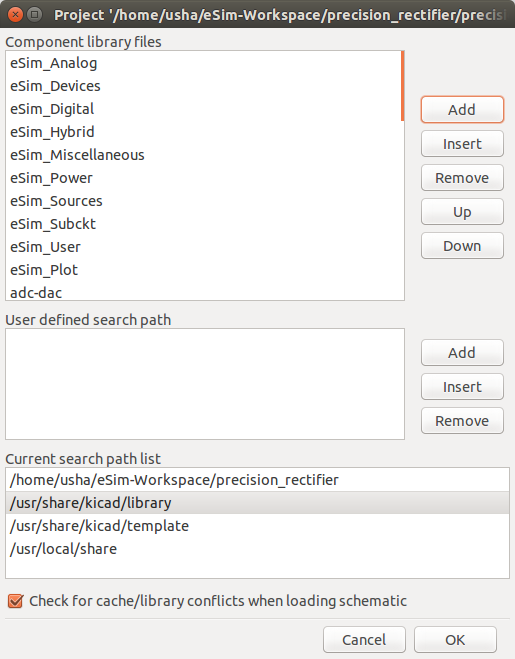
\includegraphics[width=\smfig]{manual_images/libraries.png}
\caption{eSim-Components Libraries}
\label{libraries}
\end{figure}

The following list shows the various eSim component libraries.

\begin{compactitem}
\item \textit {eSim\_Analog} - Contains Ngspice analog models such as aswitch(analog switch), summer(adder model), Transfo(Transformer), zener.
\item \textit {eSim\_Devices} -  Includes elementary components like resistor, capacitor, transistor, MosFet.
\item \textit {eSim\_Digital} -  Includes Ngspice digital models such as basic gates (AND, OR, NOR,NAND,XOR), filpflops (SR, D, JK), buffer, inverter.
\item \textit {eSim\_Hybrid} - Includes components like ADC and DAC.
\item \textit {eSim\_Miscellaneous} -  Contains components like ic(used for giving initial conditions in circuit) and port(used in creating subcircuits).
\item \textit {eSim\_Plot} -  Contains plotting components like plot\_v1 (plot voltage at a node), plot\_v2 (plot voltage between 2 nodes), plot\_i2 (plot current through branch), plot\_log (plot logarithmic voltage at a node).
\item \textit {eSim\_Power} -  Includes power components like DIAC, TRIAC and SCR.
\item \textit {eSim\_Sources} -  Contains sources for the circuits like AC voltage source, DC voltage source, sine source and pulse source.
\item \textit {eSim\_Subckt} -  Contains subcircuit components like Op-Amp(UA 741), IC 555, Half adder and full adder.
\item \textit {eSim\_User} - A repository for all user created components
\end{compactitem}

\section{Schematic creation for simulation} \index{Schematic!for
  simulation} 
There are certain differences between the schematic created for
simulation and that created for PCB design. We need certain components
like plots and current sources for simulation whereas these are not
needed for PCB design. For PCB design, we would require connectors
(e.g. DB15 and 2 pin connector) for taking signals in and out of the
PCB whereas these have no meaning in simulation. This section covers schematic creation for simulation. Refer to \chapref{chap13} to know how to create schematic for PCB design.

The first step in the creation of circuit schematic is the selection
and placement of required components. Let  us  see  this  using  an  example.   Let  us  create  the  circuit schematic of an RC  filter given in \figref{schemfin} and do a transient simulation.  


\subsection{Selection and placement of components}\index{Component!place} 
\label{selplace}
We would need a resistor, a capacitor, a voltage source, ground
terminal and some plot components. To place a resistor on the schematic editor window, select the \textit{Place a component} tool from the toolbar on the right side and click
anywhere on the schematic editor. This opens up the component
selection window. This action can also be performed by pressing
the key A. Choose the \textit{eSim\_Devices} library and click on the arrow near it. This will open the \textit{eSim\_Devices} library and the resistor component can be found here. \figref{resistor} shows the selection of resistor component. Click on {\tt OK}. A resistor will be tied to the cursor. Place the resistor on the
schematic editor by a single click. To place the next component, i.e., capacitor, click again on the schematic editor. The capacitor component is also found under \textit{eSim\_Devices} library. Select it and then click on {\tt OK}. Place the capacitor on the schematic editor by a single click.

\begin{figure}[h]
\centering
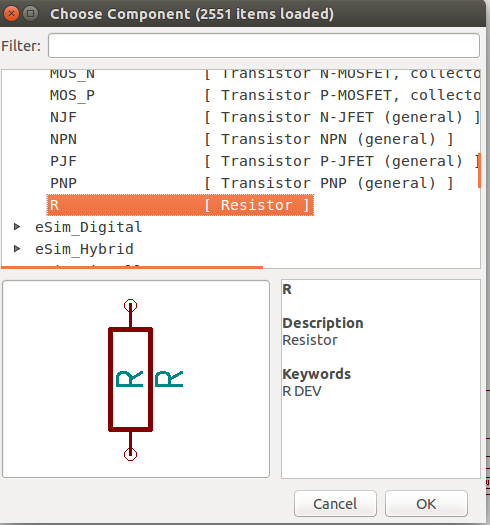
\includegraphics[width=0.5\textwidth]{resistor.png}
\caption{Placing a resistor using the Place a Component tool}
\label{resistor}
\end{figure}
 
Let us now place a sinusoidal voltage source. This is required for performing transient analysis. On the component selection window, choose the library \textit{eSim\_source}. Select the component {\tt SINE} and click on {\tt OK}. Place the sine source on the schematic editor by a single click. Similarly select and place {\tt gnd}, a ground terminal from the {\tt power} library. 

The plot components can be found under the eSim\_Plot library. Select the plot\_v1 component and place the component. Once all the components are placed, the schematic editor would look like as in \figref{afterplace}.
\begin{figure}[h]
\centering
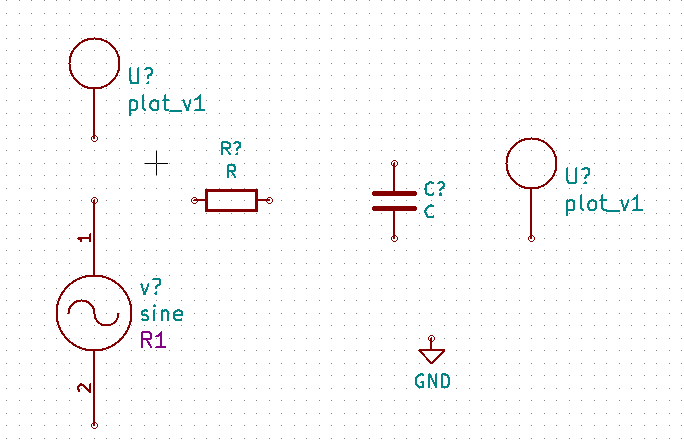
\includegraphics[width=0.63\textwidth]{manual_images/afterplace.png}
\caption{All RC circuit components placed}
\label{afterplace}
\end{figure} 

Let us rotate the resistor to complete the circuit. To rotate the resistor, place the cursor on the resistor as shown in \figref{rotate} and press the key {\tt R}. This applies to all components.\index{Component!rotate}

\begin{figure}[h]
\centering
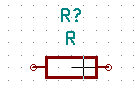
\includegraphics[width=0.3\textwidth]{manual_images/rotate.png}
\caption{Placing the cursor (cross mark) on the resistor component} 
\label{rotate}
\end{figure}

If one wants to move a component, place the cursor on top of the
component and press the key {\tt M}. The component will be tied to the
cursor and can be moved in any direction. \index{Component!move} 

\subsection{Wiring the circuit}
\index{Schematic!wiring}
The next step is to wire the connections. Let us connect the resistor
to the capacitor. To do so, point the cursor to the terminal of
resistor to be connected and press the key {\tt W}. It has now
changed to the wiring mode. Alternately, this can also be done by selecting the \textit{Place wire} tool on the right side toolbar. Move the cursor towards the terminal of
the capacitor and click on it. A wire is formed as shown in
\figref{wire1}. 
\begin{figure}[h]
\centering
\subfloat[Initial stages]{
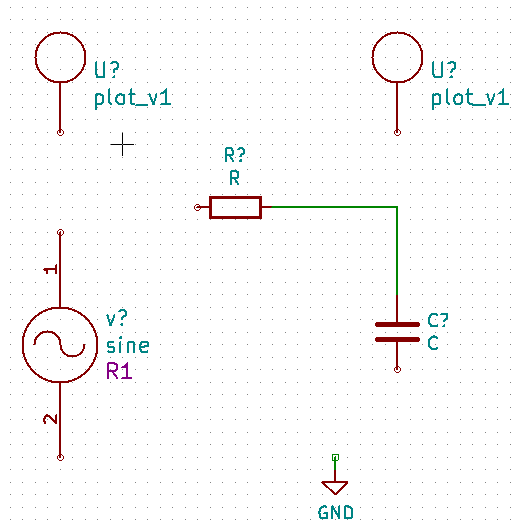
\includegraphics[width=\tnfig]{manual_images/wire1.png}
\label{wire1}} \hfill
\subfloat[Wiring done]{
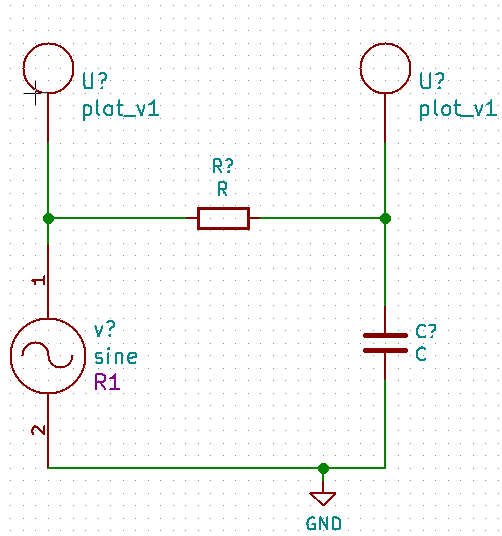
\includegraphics[width=\tnfig]{manual_images/wirefin.png}
\label{wirefin}} \hfill
\subfloat[Final schematic with PWR\_FLAG]{
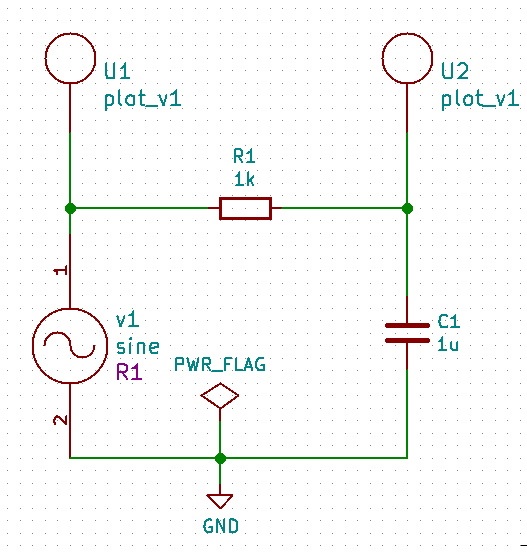
\includegraphics[width=\tnfig]{manual_images/schemfin.png}
\label{schemfin}}
\caption{Various stages of wiring}
\end{figure}
Similarly connect the wires between all terminals and the final
schematic would look like \figref{wirefin}. 

\subsection{Assigning values to components}\index{Component!values}
We need to assign values to the components in our circuit i.e.,
resistor and capacitor. Note that the sine voltage source has been
placed for simulation. The specifications of sine source will be given
during simulation. 
To assign value to the resistor, place the cursor above the letter {\tt R}
(not {\tt R?}) and press the key {\tt E}. Choose \textit{Field
  value}. Type {\tt 1k} in the \textit{Edit value field} box as shown
in \figref{field}. 1k means $1k\Omega$. Similarly give the value
{\tt 1u} for the capacitor. 1u means $1\mu F$.  

\begin{figure}[h]
\centering
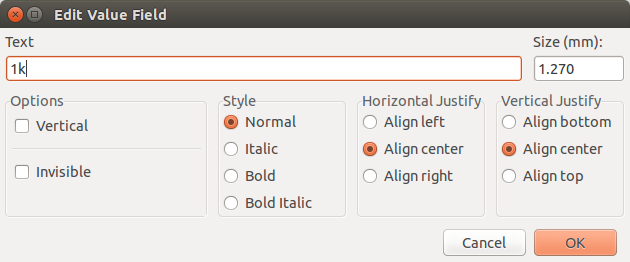
\includegraphics[width=0.5\textwidth]{manual_images/field.png}
\caption{Editing value of resistor}
\label{field}
\end{figure}

\subsection{Annotation and ERC}
\label{ann}\index{Annotate}\index{Schematic!annotate}\index{ERC} \index{Schematic!ERC}
The next step is to annotate the schematic. Annotation gives unique
references to the components. To annotate the schematic, click on
\textit{Annotate Schematic Components} tool from the top toolbar. Click on
{\tt Annotate}, then click on {\tt OK} and finally click on Close as shown in
\figref{anno}. The schematic is now annotated. The question marks
next to component references have been replaced by unique numbers. If
there are more than one instance of a component (say resistor), the
annotation will be done as R1, R2, etc. 

\begin{figure}[h]
\centering
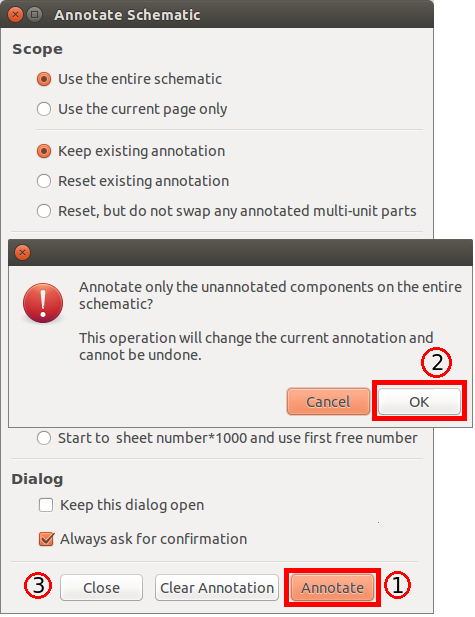
\includegraphics[width=0.45\textwidth]{manual_images/anno.png}
\caption{Steps in annotating a schematic: 1. First click on Annotation then 2. Click on OK then 3. Click on close}
\label{anno}
\end{figure}

Let us now do {\tt ERC} or {\tt Electric Rules Check}. To do so, click
on \textit{Perform electric rules check} tool from the top
toolbar. Click on \textit{Run} button. The error as shown in
\figref{erc} may be displayed. Click on close in the test
erc\index{ERC} window. \index{ERC!error}

\begin{figure}[h]
\centering
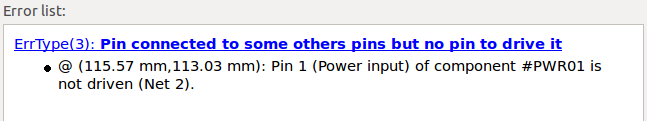
\includegraphics[width=\lgfig]{manual_images/erc2.png}
\caption{ERC error}
\label{erc}
\end{figure}

There will be a green arrow pointing to the source of error in the
schematic. Here it points to the ground terminal. This is shown in
\figref{ercgnd}.

\begin{figure}[h]
\centering
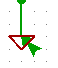
\includegraphics[width=0.1\textwidth]{ercgnd.png}
\caption{Green arrow pointing to Ground terminal indicating an ERC error}
\label{ercgnd}
\end{figure}

This error is due ti the GND pin. The GND pin is a power input pin and Eeschema gives this error as there is no power line connected. To correct this error, a flag has to be placed indicating that there will be an external power line connected to it. Place a {\tt PWR\_FLAG} from the Eeschema 
library \textit{power}. \index{Power Flag} Connect the power flag to the
ground terminal as shown in \figref{schemfin}. %More information about
%PWR\_FLAG is given in \secref{pwr}. One needs to place {\tt PWR\_FLAG}wherever the error shown in \figref{erc} is obtained. 
Repeat the ERC. Now there are no errors. With this we have created the schematic for simulation.

\subsection{Netlist generation}\index{Netlist!for simulation}
\label{chap5-netlist-generation}
To simulate the circuit that has been created in the previous section, we
need to generate its netlist. {\tt Netlist} is a list of components in
the schematic along with their connection information. \index{Netlist}
To do so, click on the \textit{Generate netlist} tool from the top
toolbar. Click on Spice from the window that opens up. Check the
option {\tt Default Format}. Then click on
\textit{Generate}. This is shown in \figref{chap5net}. Save the
netlist. This will be a {\tt .cir} file. Do not change the directory
while saving. 
\begin{figure}[h]
\centering
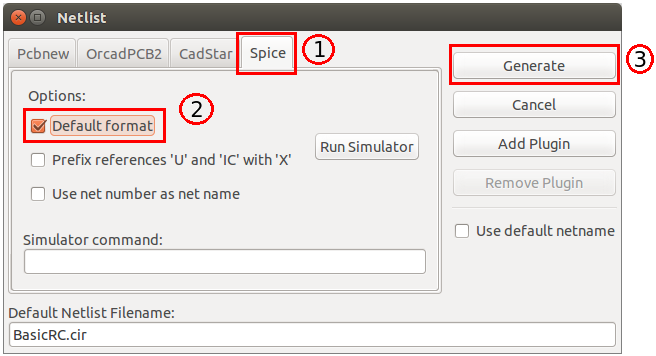
\includegraphics[width=0.6\textwidth]{manual_images/netlist.png}
\caption{Steps in generating a Netlist for simulation: 1. Click on Spice then\\
 2. Check the option {\tt Default Format} then 3. Click on Generate}
\label{chap5net}
\end{figure} 
Now the netlist is ready to be simulated. 
% Refer to \cite{kicad} or \cite{kicad2} to know more about Eeschema.

\section {Tools for creating the PCB layout}
The Eeschema top toolbar also has two important tools which can help the user to generate the PCB layout of the created schematic.

\subsection {FootPrint Editor}
Clicking on the \textit{Footprint Editor} tool will open the {\tt CvPcb} 
\index{CvPcb} window. This window will ideally open the .net file for the 
current project. So, before using this tool, one should have the netlist 
for PCB design (a .net file). To know more about how to assign footprints 
to components, see \chapref{chap13}.

\subsection {PCB Layout}
Clicking on the \textit{Layout Editor} tool will open {\tt
Pcbnew}\index{Pcbnew}, the layout editor used in eSim. In this
window, one will create the PCB. It involves laying tracks and vias,
performing optimum routing of tracks, creating one or more copper
layers for PCB, etc. It will be saved as a {\tt .brd} file in the 
current project directory. \chapref{chap13} explains how to use the 
\textit{Layout Editor} to design a PCB. 


%\printindex
%\end{document}
 % adds chapter 5
\chapter{Simulation}
\thispagestyle{empty}
\label{chap6}

Circuit simulation \index{Circuit simulation} uses mathematical models
to replicate the behaviour of an actual device or circuit. Simulation
software allows to model circuit operations. Simulating a
circuit's behaviour before actually building it can greatly improve
design efficiency. eSim uses {\tt Ngspice}\index{Ngspice} for analog, digital and
mixed-level/mixed-signal circuit simulation. The various steps involved in simulating a circuit schematic in eSim are explained in the sections below:

\section {Kicad to Ngspice Conversion}
In the chapter on schematic creation, we have learnt to generate the netlist from circuit schematic. The generated netlist is not compatible with Ngspice. eSim uses Ngspice to simulate the circuit schematic. Hence the netlist i.e. {\tt .cir} file generated should be converted in to a  Ngspice compatible file. The \textit{Convert KiCad to Ngspice} tool on eSim left toolbar is used to do this. Let us now see the various tabs and their functions available under this.   

\subsection {Analysis} \label{ana}
In order to simulate a circuit, the user must define the type of
analysis to be done on the circuit. This tab is used to insert the type of analysis and  value of the analysis parameters to the netlist. eSim supports three types of analyses:
\begin{inparaenum}
\item \textit {DC Analysis} (Operating Point and DC Sweep) \index{DC Analysis}
\item \textit {AC Small-signal Analysis} \index{AC Small-signal Analysis} 
\item \textit {Transient Analysis} \index{Transient Analysis}
\end{inparaenum}
These are explained below. %\cite{ngspice}.

\begin{figure}
\centering
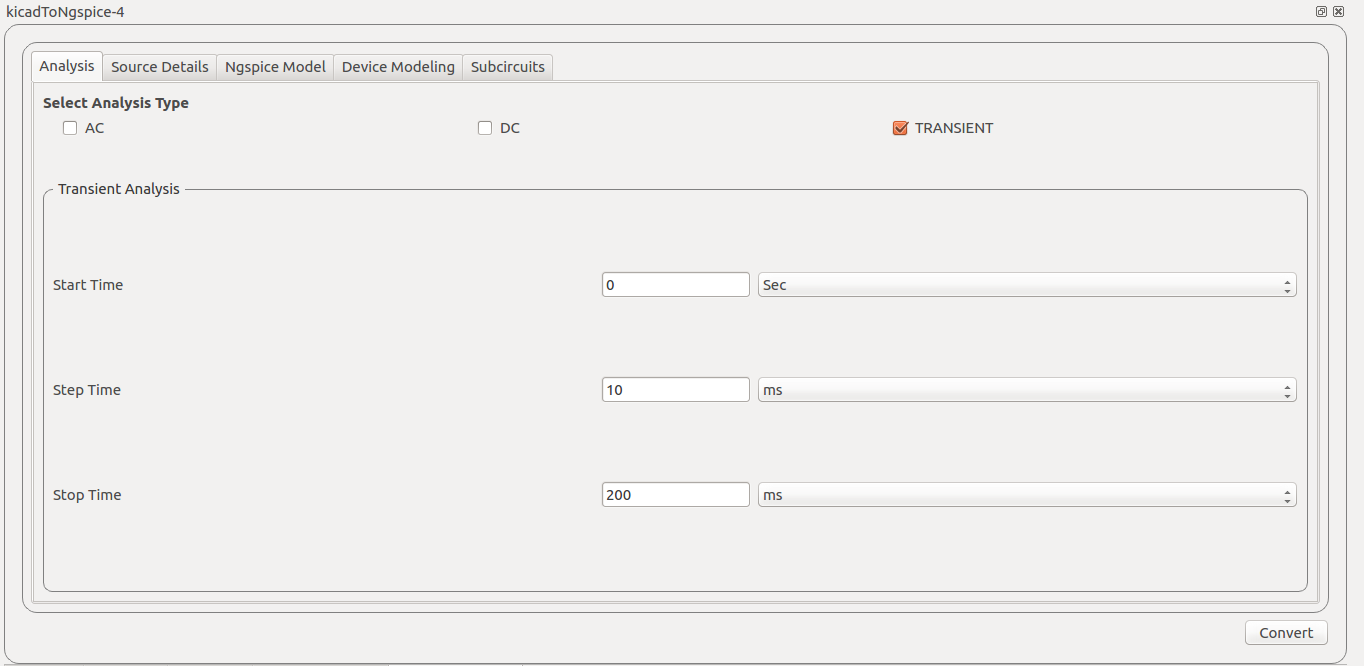
\includegraphics[width=\lgfig]{analysis.png}
\caption{KiCad to Ngspice Window}
\label{analysis}
\end{figure}

In the current example for simulating an RC circuit, select the analysis type as {\tt transient} analysis and enter the values as shown in the \figref{analysis}.  

\begin{comment}
Analysis Inserter generates the commands for Ngspice. When one clicks
on \textit {Kicad to Ngspice} from the eSim toolbar, one gets
the Analysis Inserter GUI as shown in \figref{1}. The various tabs in
this GUI correspond to the various types of analysis. The user can
enter the details, needed to perform simulation, in the corresponding
fields under these tabs.

\subsubsection{DC analysis} \index{DC Analysis} The {\tt DC analysis}
determines the dc operating point of the circuit with inductors
shorted and capacitors opened. It is assumed that there is no time dependence on any of the sources within the system description. The simulator algorithm subdivides the circuit into those portions which require the {\tt analog simulator algorithm} and
those which require the {\tt event-driven algorithm}. Each subsystem block
is then iterated to solution, with the interfaces between analog nodes
and event-driven nodes iterated for consistency across the entire
system. Once stable values are obtained for all nodes in the system, the
analysis halts and the results could be displayed or printed out.
 
A {\tt DC analysis} is automatically performed prior to a {\tt transient analysis}
to determine the transient initial conditions, and prior to an {\tt ac
small-signal analysis} to determine the linearized, small-signal models
for nonlinear devices.  The {\tt DC analysis} can also be used to generate
dc transfer curves: a specified independent voltage or current source
is stepped over a user-specified range and the dc output variables are
stored for each sequential source value.

\subsubsection{AC small-signal analysis}\index{AC Small-signal Analysis}
{\tt AC analysis} is limited to analog nodes. It represents the small
signal, sinusoidal solution of the analog system described at a
particular frequency or set of frequencies. This analysis is similar
to the {\tt DC analysis} in that it represents the steady-state behaviour of
the described system with a single input node at a given set of
stimulus frequencies.

The program first computes the dc operating point of the circuit and
determines linearized, small-signal models for all of the nonlinear
devices in the circuit. The resultant linear circuit is then analyzed
over a user-specified range of frequencies. The desired output of an
ac small-signal analysis is usually a transfer function (voltage gain,
trans impedance, etc.). If the circuit has only one ac input, it is
convenient to set that input to unity and zero phase, so that output
variables have the same value as the transfer function.

\subsubsection{Transient analysis}\index{Transient Analysis}
{\tt Transient analysis} is an extension of {\tt DC analysis} to the time
domain. A {\tt transient analysis} begins by obtaining a DC solution to
provide a point of departure for simulating time-varying
behaviour. Once the DC solution is obtained, the time-dependent aspects
of the system are reintroduced and the simulator algorithms
incrementally solve for the time varying behaviour of the entire
system. Inconsistencies in node values are resolved by the simulation
algorithms such that the time-dependent waveforms created by the
analysis are consistent across the entire simulated time interval.

Resulting time-varying descriptions of node behaviour for the specified
time interval are accessible. All sources which are not time
dependent (for example, power supplies) are set to their dc value. The
transient time interval is specified on a \textit {.tran} control line.  


\subsection{DC analysis inserter}
By default {\tt DC analysis} option appears when one clicks on \textit {Analysis
Inserter}. Here we need to give the details of input \textit {source name}, \textit {start
value} of input, \textit {increment} and \textit {stop} value. Once this is done, click on \textit {Add
Simulation Data}.

\figref{2} gives an example of {\tt DC analysis} inserter.  In this example,
{\tt v1} is the input voltage source which \textit {starts} at {\tt 0
  Volt}, \textit {increments} by {\tt 1 Volt} and \textit {stops} at
{\tt 10 Volt}. On clicking \textit {Add Simulation Data}, the analysis
command is generated and is of the form:
\\
{\tt.dc\index{.dc} sourcename vstart vstop vincr}
\\
The {\tt .dc} line defines the dc transfer curve source and sweep
limits (with capacitors open and inductors shorted). {\tt srcnam} is
the name of an independent voltage or current source. {\tt vstart},
{\tt vstop}, and {\tt vincr} are the starting, final, and incrementing
values respectively, of the source.

When we check the option \textit {Operating Point
  analysis}\index{Operating point analysis} on the DC analysis window,
{\tt .op} gets appended to the analysis statement.
\begin{figure}[ho]
\centering
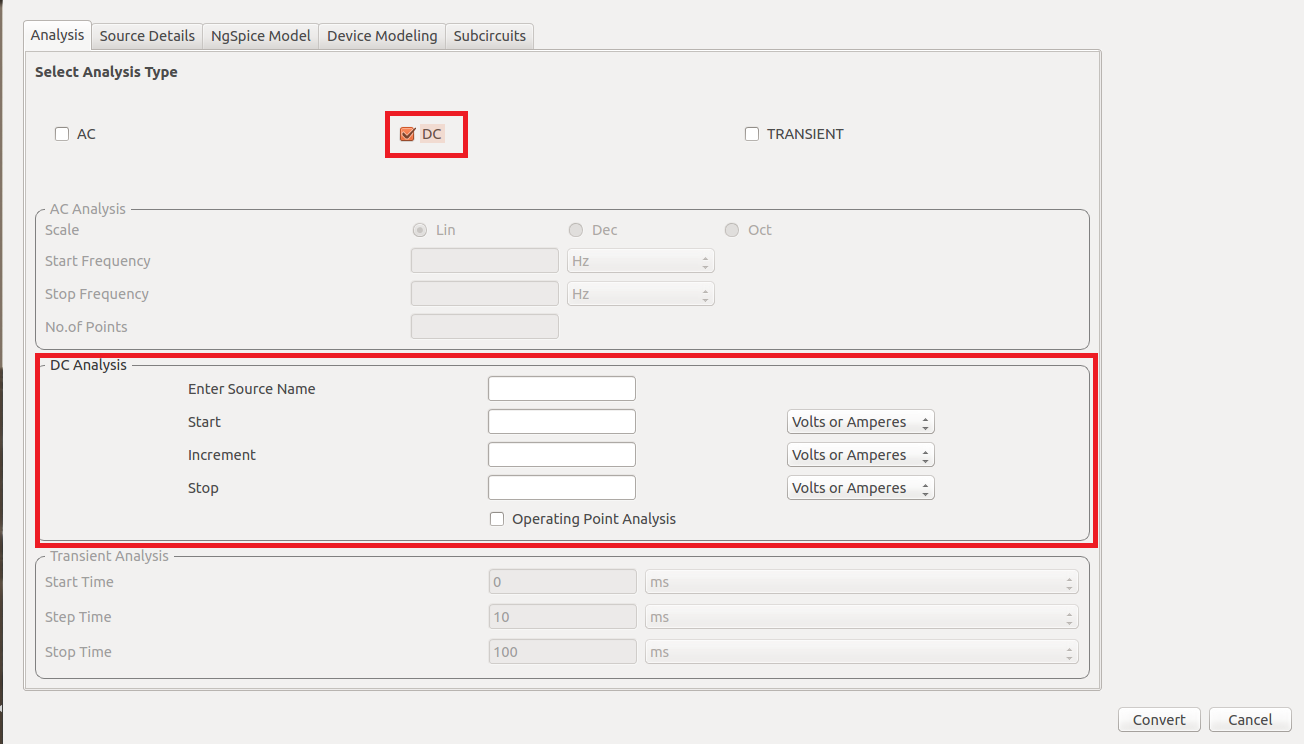
\includegraphics[width=0.475\linewidth]{figures/dc1.png}
\caption{DC Analysis GUI}
\label{2}
\end{figure}
The inclusion of the line {\tt .op} in the analysis file directs
Ngspice to determine the dc operating point of the circuit with
inductors shorted and capacitors opened.

\subsection{AC analysis inserter}\index{AC Analysis Inserter}
When one clicks on the option \textit {AC} in the \textit {Analysis Inserter} GUI, the
window given in \figref{4} appears.
\begin{figure}[ho]
\centering
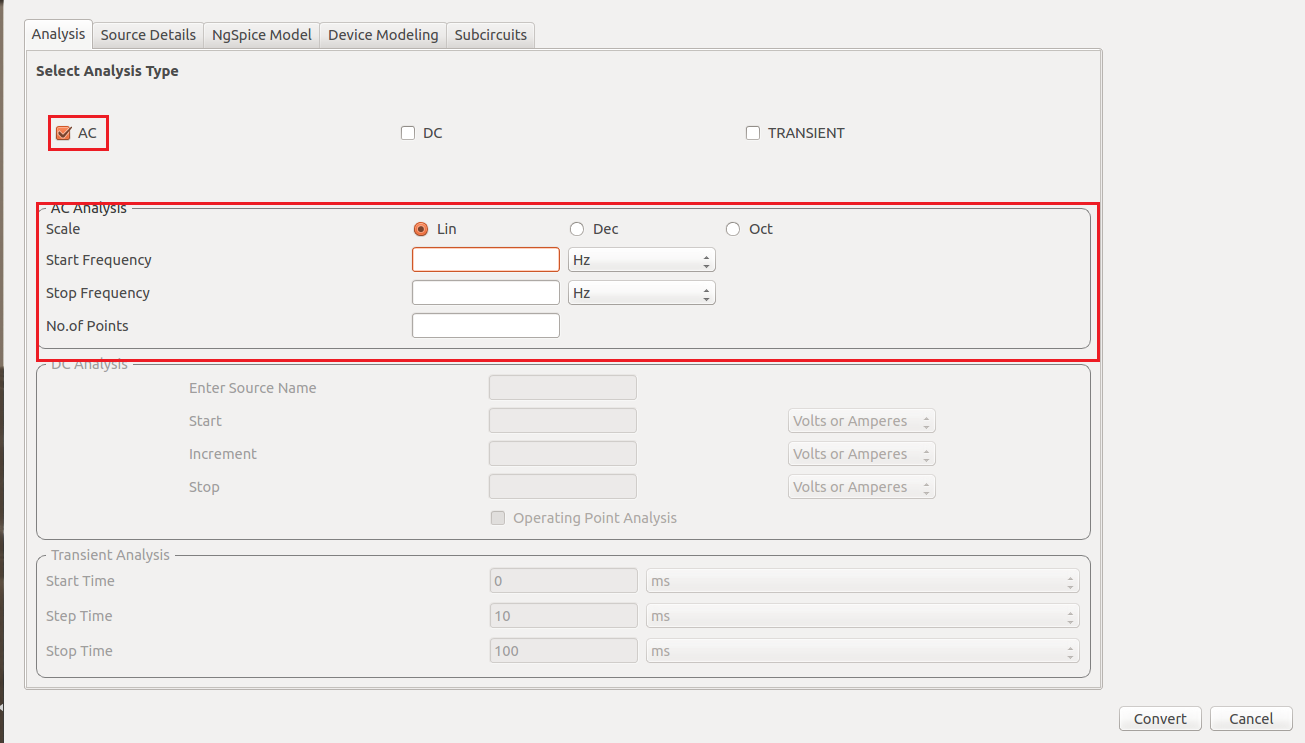
\includegraphics[width=\smfig]{figures/ac1.png}
\caption{AC Analysis GUI}
\label{4}
\end{figure}
Here one needs to enter the details of \textit {scale}, \textit {start
  frequency}, \textit{stop frequency} and \textit {Number of points}. 

After entering these values, click on \textit {Add Simulation
  Data}. The analysis statement is generated. This is in one
of the three forms listed below, depending on the type of \textit
{scale} that one chooses. The types of \textit {scale} available are
\textit {dec}, \textit {oct}, and \textit {lin}, the usage of which is
explained below: \\
{\tt .ac dec nd fstart fstop }\\
{\tt .ac oct no fstart fstop }\\
{\tt .ac lin np fstart fstop } \index{.ac} \\
Here, {\tt dec} stands for decade
variation and {\tt nd} is the number of points per decade. {\tt oct}
stands for octave variation and {\tt no} is the number of points per
octave. {\tt lin} stands for linear variation and {\tt np} is the number of
points. {\tt fstart} is the starting frequency and {\tt fstop} is the
final frequency.

If the {\tt .ac} analysis is included in the analysis file, Ngspice
performs an AC analysis of the circuit over the specified frequency
range. Note that in order for this analysis to be meaningful, at least
one independent source must have been specified with an ac value. While creating the schematic for performing ac analysis, add the component {\tt AC} from the \textit{sourcesSpice} library.

\subsection{Transient analysis inserter}\index{Transient Analysis
  Inserter}
When one clicks on the option \textit {Transient} in the \textit {Analysis Inserter}
GUI, the window given in \figref{6} appears.  Here one needs to
enter the details of \textit {start time}, \textit {step time}, and \textit {stop
  time}.  After entering these values, click on \textit {Add Simulation
Data}. The analysis statement is generated. It is of the
form:

{\tt .tran tstep tstop tstart}\index{.tran}

Here, {\tt tstep} is the printing or plotting increment for
line-printer output. For use with the post-processor, {\tt tstep} is
the suggested computing increment. {\tt tstop} is the final time, and
{\tt tstart} is the initial time. If tstart is omitted, it is assumed
to be zero.

The transient analysis always begins at time zero. In the interval
{\tt \textless zero, tstart\textgreater}, the circuit is analyzed (to
reach a steady state), but no outputs are stored. In the interval {\tt
  \textless tstart, tstop\textgreater}, the circuit is analyzed and
outputs are stored.
\begin{figure}[ho]
\centering
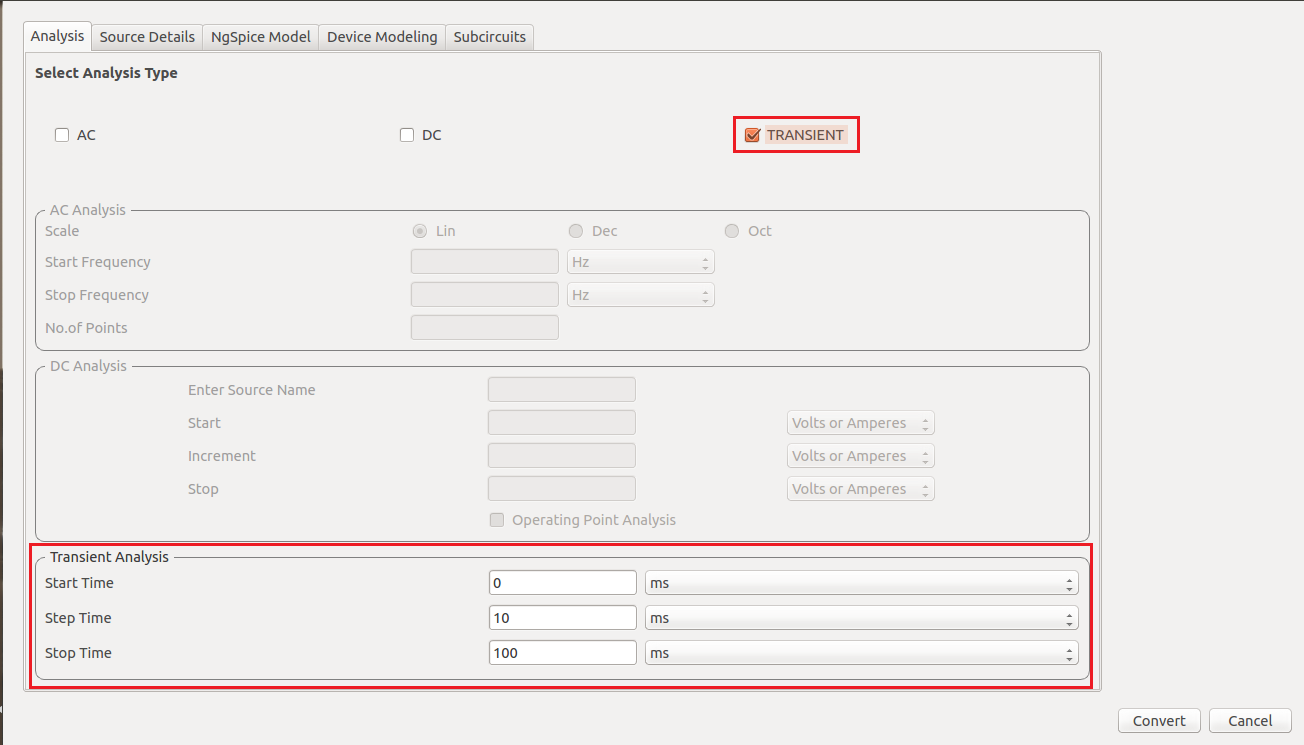
\includegraphics[width=\smfig]{figures/trans1.png}
\caption{Transient Analysis GUI}
\label{6}
\end{figure}


\begin{enumerate}
\item \textit {Analysis} - This tab is used to insert the type of analysis and  value of the analysis parameters to the netlist.
\item \textit {Source Details} - The netlist created in the \textit{Schematic Editor} is converted to 
  Ngspice format and analysis commands is appended to it. It is done
  by the \textit{Netlist Converter} tool in the eSim
  toolbar. \index{Netlist Converter}
\item Ngspice Modelling \index{Ngspice simulation} - Ngspice
  simulation of the netlist is performed. It is done by clicking on the \textit{Ngspice} tool in the eSim toolbar.
\item Model Library - Model library adds the component library of the components like Diode, JFET, MOS, IGBT. These library file contains the parameters and the values of the components.

\item Sub-Circuit - A sub circuiting can be done using this tool. This involves adding the sub circuit used in the main circuit. This adds all the project files of the sub circuit.
\end{enumerate}
\end{comment}

\subsection {Source Details} \label{source}
The various parameter values of the sources added in the schematic can added using this tool. \textit {Source details} is a dynamic tab, i.e. the fields are added as per the number of sources in the circuit. For example, consider a Half-Adder circuit as shown in \figref{halfschematic}
\begin{figure}
\centering
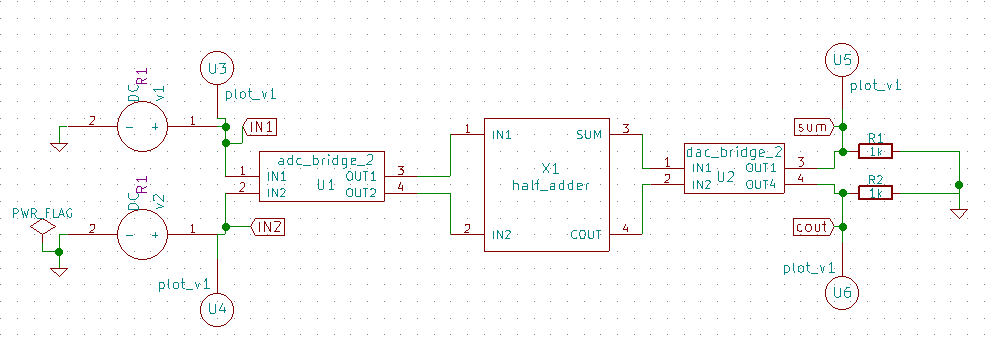
\includegraphics[width=\lgfig]{manual_images/half-adder.png}
\caption{Half Adder Schematic}
\label{halfschematic}
\end{figure}
Here, we have used two DC input sources are used and hence the source detail GUI would be having two input fields as shown is \figref{sourcehalfadder}.

\begin{figure}[h]
\centering
\subfloat[Source Details of Half-Adder]{
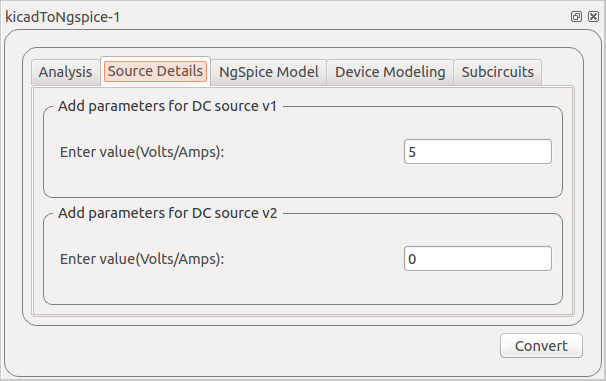
\includegraphics[width=\smfig]{manual_images/source-details.png}
\label{sourcehalfadder}} \hfill
\subfloat[Source Details of RC circuit]{
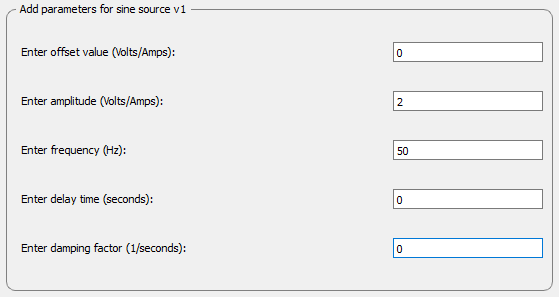
\includegraphics[width=\smfig]{manual_images/rc-sourcedetails.PNG}
\label{sourcerc}} \hfill
\caption{Source details interface}
\end{figure}

In the current example of the RC circuit, we have a single AC source. Fill in the details as shown in \figref{sourcerc}.

\subsection {Ngspice Model} \label{ngspicemodel}
The component libraries for components like DAC, ADC, transformer etc. which are used in the schematic are directly linked with the corresponding Ngspice models. The user can modify the parameter values using this tab, as shown in \figref{ngspicemodel}. If there are no modifications the default values are taken.

\begin{figure}
\centering
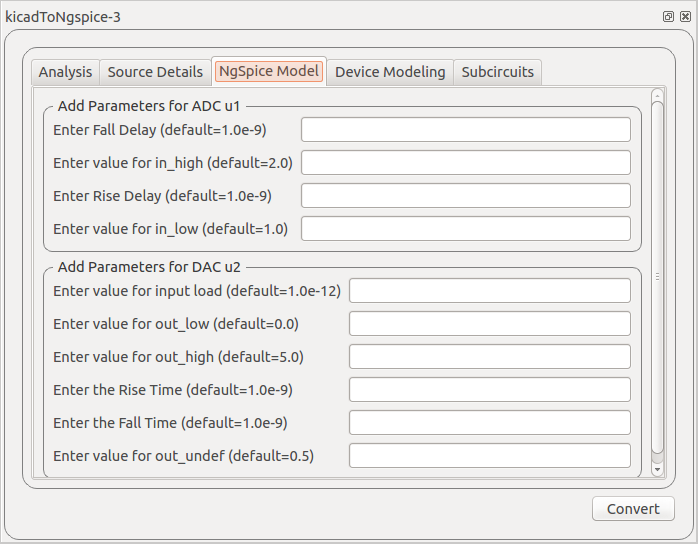
\includegraphics[width=\lgfig]{manual_images/ngspice-model.png}
\caption{Half adder: Ngspice model}
\label{ngspicemodel}
\end{figure}

\subsection {Device Modelling} \label{devicemodel}
Spice based simulators include a feature which allows accurate modeling of semiconductor devices such as diodes, transistors etc. Model libraries holds these features to define models for devices such as diodes, MOSFET, BJT, JFET, IGBT, Magnetic core etc.

The fields in this tab are added for each such device in the circuit and the corresponding model library is added. In the example of bridge rectifier as shown in \figref{bridgerectifier} for four diodes library files are added as in \figref{devicemodel}. Location for these libraries is as following : \\
../Library/deviceModelLibrary/Diode/ if you are using version 2.0 and above \\
../src/deviceModelLibrary/Diode/ if you are using versions lower than 2.0

\begin{figure}[h]
\centering
\subfloat[Schematic]{
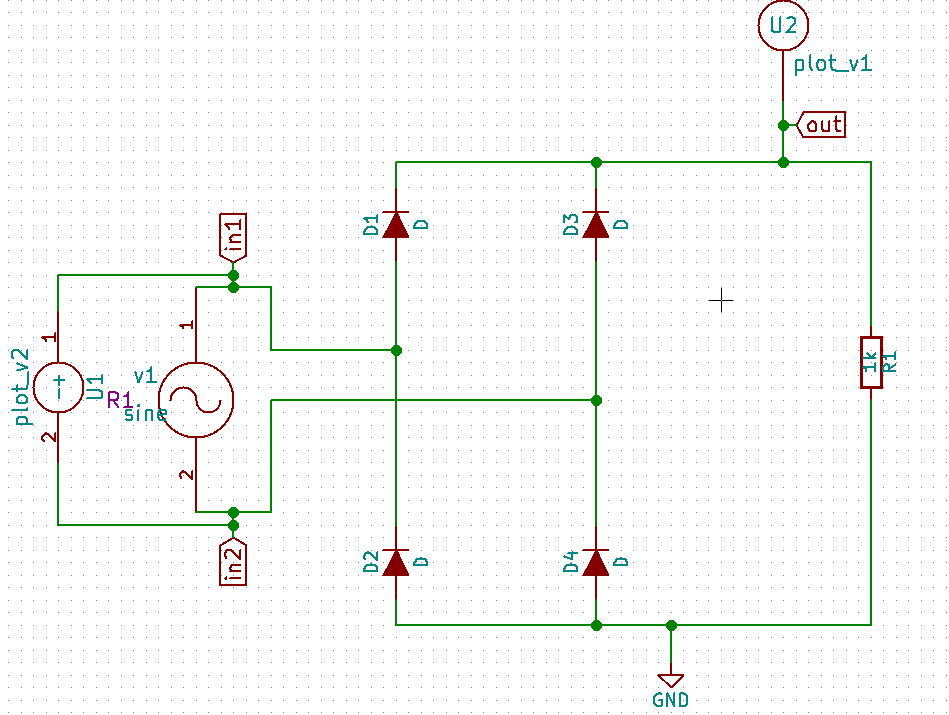
\includegraphics[width=\smfig]{manual_images/bridgerectifier.png}
\label{bridgerectifier}} \hfill
\subfloat[Adding device model]{
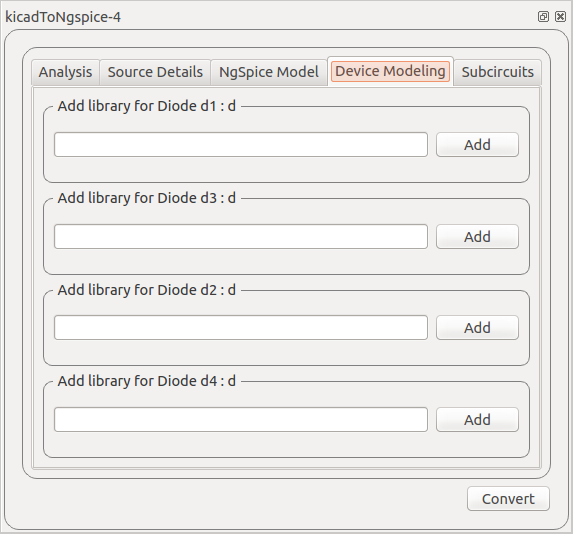
\includegraphics[width=\smfig]{manual_images/devicemodel.png}
\label{devicemodel}} \hfill
\caption{Bridge Rectifier}
\end{figure}

\subsection{Sub Circuit}
Subcircuit is a way to implement hierarchical modeling.  Once a subcircuit for a compo-
nent is created, it can be used in other circuits. \\
In the KiCadToNgspice conversion of example 7805VoltageRegulator, where a bridge rectifier is further connected to a voltage regulator LM7805, a subcircuit of this 7805 IC is used. These are located in library/Subcircuitlibrary if you are using version 2.0 and above and in src/SubcircuitLibrary if you are using versions lower than 2.0. The association is done as shown in \figref{7805}.
\begin{figure}
\centering
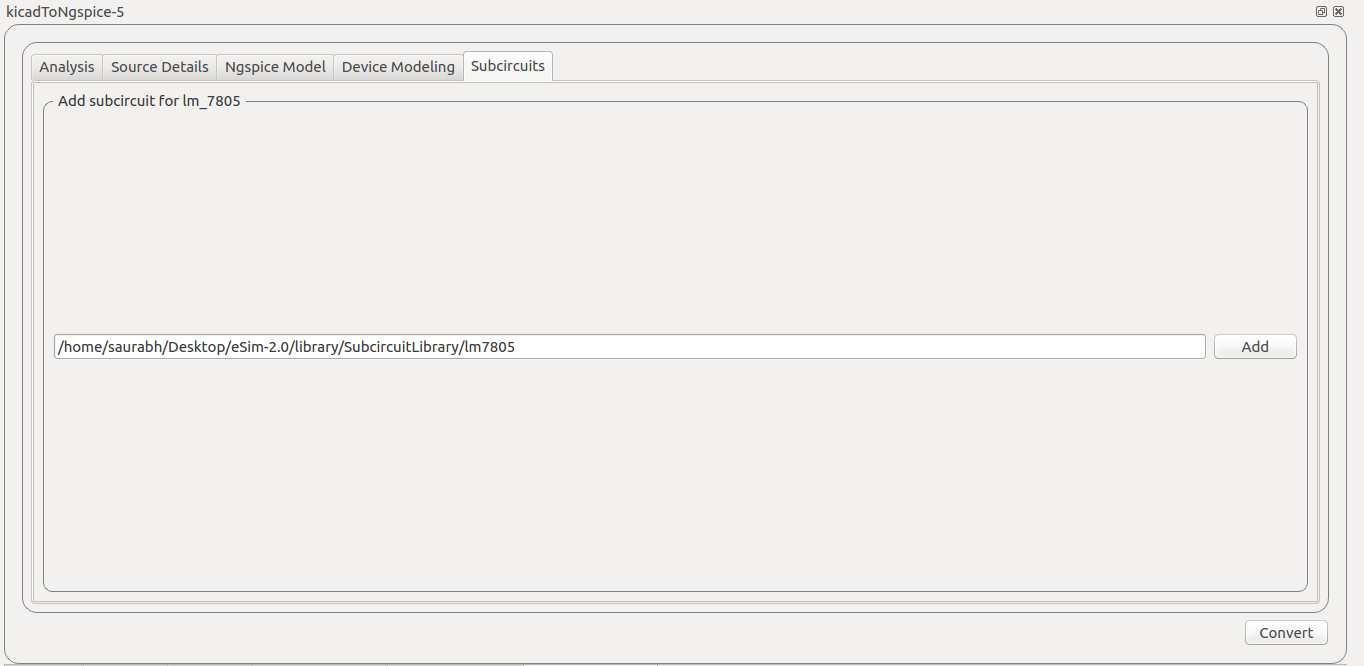
\includegraphics[width=\lgfig]{7805.png}
\caption{Assigning appropriate subcircuit file }
\label{7805}
\end{figure}
\\
\begin{comment}
The field in this tab are added for each such component in the circuit and the corresponding subcirucit is added. . as shown in \figref{bridgerectifier} for component Half_Adder the file is added as in \figref{devicemodel}.  
-------Just need to change the images------------
\begin{figure}[h]
\centering
\subfloat[Schematic]{
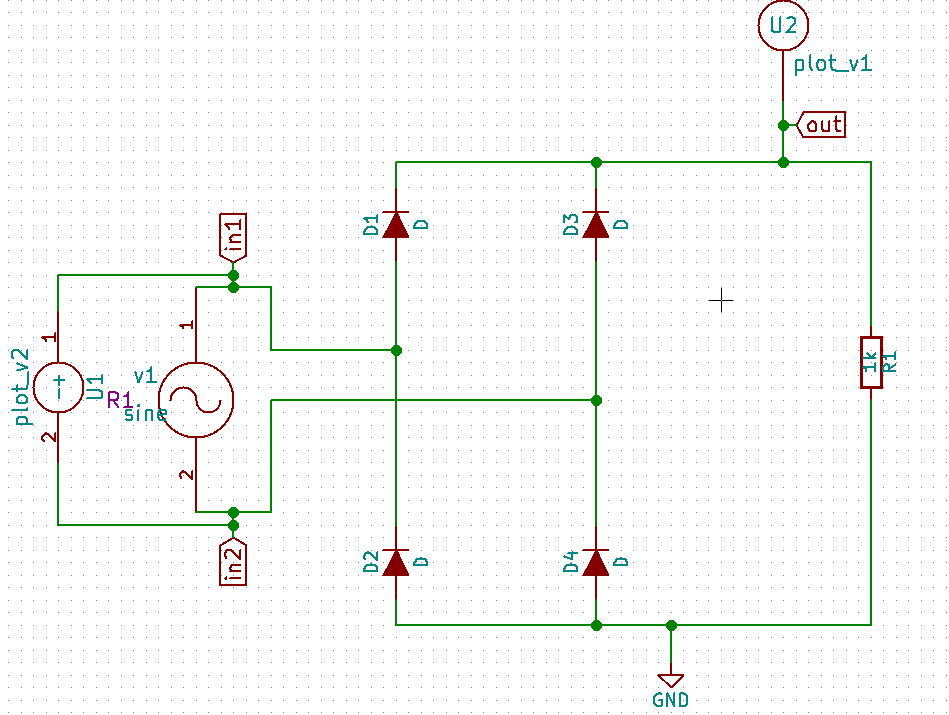
\includegraphics[width=\smfig]{manual_images/bridgerectifier.png}
\label{bridgerectifier}} \hfill
\subfloat[Adding device model]{
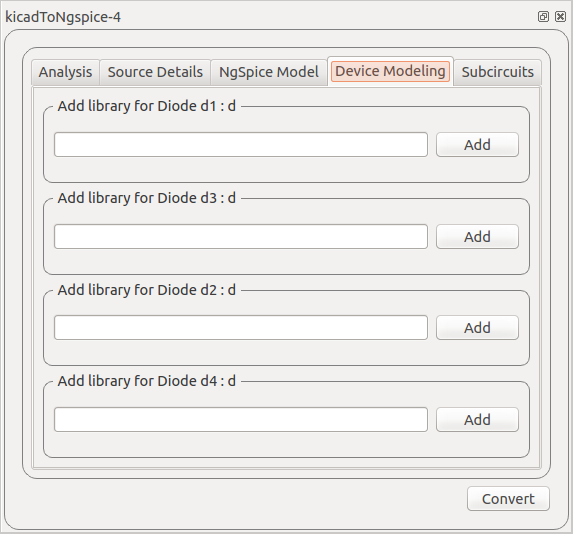
\includegraphics[width=\smfig]{manual_images/devicemodel.png}
\label{devicemodel}} \hfill
\caption{Bridge Rectifier}
\end{figure}
\end{comment}


After Filling up the values in all the above mentioned fields the convert button is pressed. The Ngspice netlist, {\tt .cir.out} file is generated. A message box pops up, as shown in \figref{success}. Click on {\tt OK}.

\begin{figure}
\centering
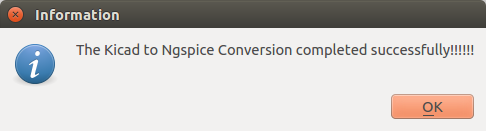
\includegraphics[width=\lgfig]{manual_images/success.png}
\caption{Message after successful Ngspice netlist generation}
\label{success}
\end{figure}

\section{Simulating the schematic}
\subsection{Simulation}
Once the Kicad to Ngspice conversion is successfully completed, press the \textit{Simulation} button on the leftside toolbar on eSim interface. This will display the Python plot window along with the node names. Select the required nodes and click on {\tt Plot}. The simulations are displayed. In the present example of the RC circuit, the plot will be displayed as shown in \figref{rc-python}.  By changing the values of capacitor and resistor, the output can be varied.We can also use the option {\tt Function} from the right side of the python plot window to plot combination of waveforms for example {\tt plot V1+V2}.

\begin{figure}
\centering
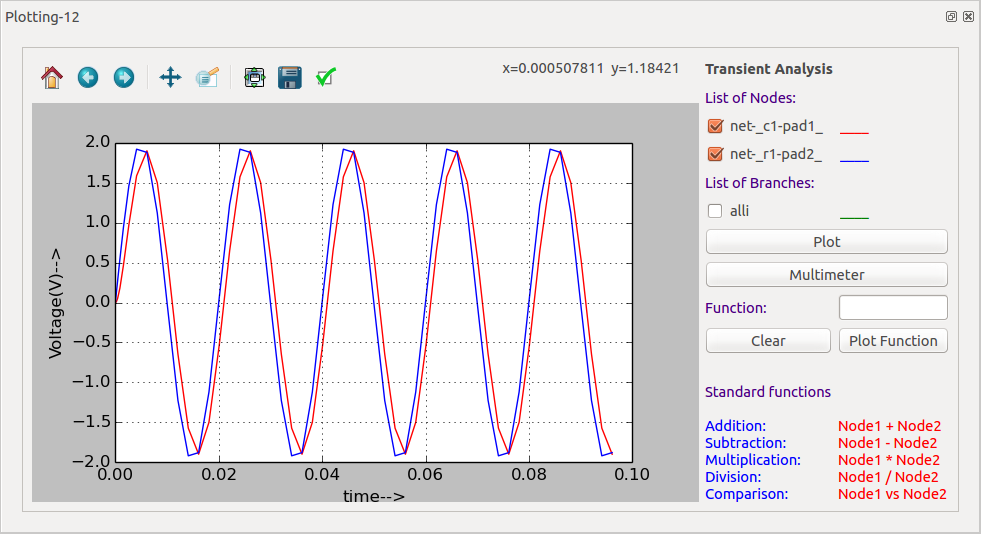
\includegraphics[width=\lgfig]{manual_images/rc-python.png}
\caption{Pythonplot for RC circuit}
\label{rc-python}
\end{figure}

Pressing the \textit{Simulation} button also opens up the Ngspice terminal and plot windows. The Ngspice plots for all the nodes (where we have used the plot components in the schematic) will be displayed. In the current example, we have used two plot components and the Ngspice simulations for these two nodes are displayed as in \figref{rc-voltage}.

\begin{figure}
\centering
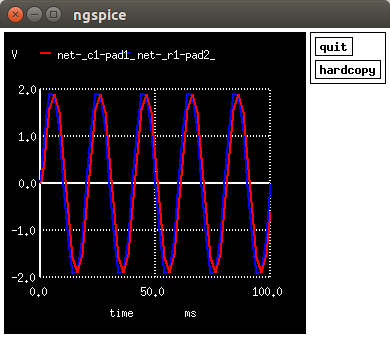
\includegraphics[width=\lgfig]{manual_images/rc-voltage.png}
\caption{Ngspice voltage simulation for RC circuit}
\label{rc-voltage}
\end{figure}

If the \textit{Plot components} are not used in the schematic, the simulations are not displayed automatically. To see the Ngspice simulations, type the following commands in the Ngspice terminal window.
\begin{itemize}
\item \textbf{plot allv} - Plots all the voltage waveforms.
\item \textbf{plot v(node-name)} - Plot a waveform of the node-name voltage source e.g. \textbf{plot v(out)} will plot the voltage at node \textbf{out} 
\item \textbf{plot v(node-one) v(node-two)} - Plots waveforms of voltages at node-one and node-two on a single graph. Multiple nodes can be observed in a single graph, though scaling has to be kept in mind. 
\item \textbf{plot alli} - Plots all the current waveforms.

You can refer the ngspice commands from {\tt https://esim.fossee.in/ngspicecmd}
\end{itemize}

\subsection{Multimeter}
Multimeter is another feature that is available in eSim. Using this facility the user can view the voltage and current values in various nodes and branches respectively. To use the multimeter select the required nodes from the plot window and press {\tt Multimeter} button, shown in \figref{multimeter}. Windows equal to the number of selected nodes will open. Now open the schematic window and place these pop up windows near the appropriate nodes on the schematic to get the voltage of each node. Similarly current through each branches in the schematic can also be found using the multimeter facility.

\begin{figure}
\centering
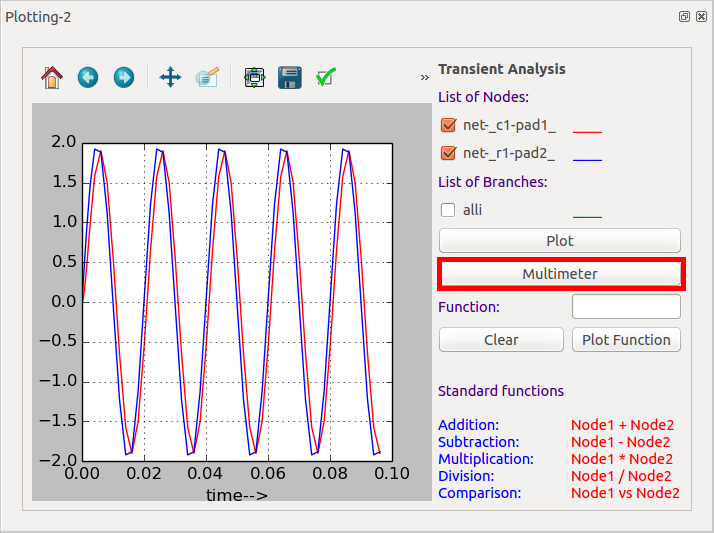
\includegraphics[width=\lgfig]{manual_images/multimeter.png}
\caption{Multimeter feature in eSim}
\label{multimeter}
\end{figure}


 % adds chapter 6
\chapter {Model Editor}
\label{chap7}
\thispagestyle{empty}

Spice based simulators include a feature which allows accurate modeling
of semiconductor devices such as diodes, transistors etc. eSim Model
Editor provides a facility to define a new model for devices such as
\textit{diodes, MOSFET, BJT, JFET, IGBT, Magnetic core} etc. Model Editor in
eSim lets the user enter the values of parameters depending on the type of 
device for which a model is required. The parameter values can be
obtained from the data-sheet of the device. A newly created model can be
exported to the model library and one can import it for different
projects, whenever required. Model Editor also provides a facility to
edit existing models. The GUI of the model editor is as shown in \figref{modeleditor}

\begin{figure}
\centering
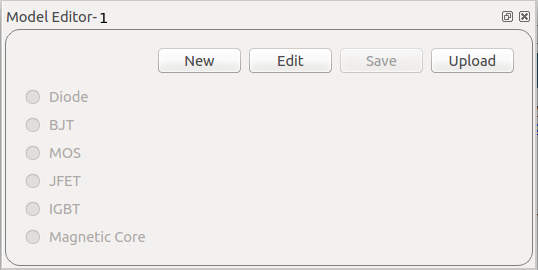
\includegraphics[width =\lgfig]{modeleditor_new.png}
\caption{Model Editor}
\label{modeleditor}
\end{figure} 

\section{Creating New Model Library }

eSim lets us create new model libraries based on the template model libraries.
On selecting {\tt New} button the window is popped as shown in \figref{modeleditor_new}. The name has to be unique otherwise the error message appears on the window.

\begin{figure}
\centering
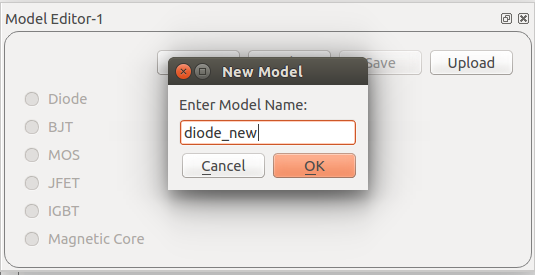
\includegraphics[width =\lgfig]{modeleditor.png}
\caption{Creating New Model Library}
\label{modeleditor_new}
\end{figure}
After the OK button is pressed the type of model library to be created is chosen by selecting one of the types on the left hand side i.e.{ \tt Diode, BJT, MOS, JFET, IGBT, Magnetic Core}. The template model library opens up in a tabular form as shown in \figref{modelnew}
\begin{figure}
\centering
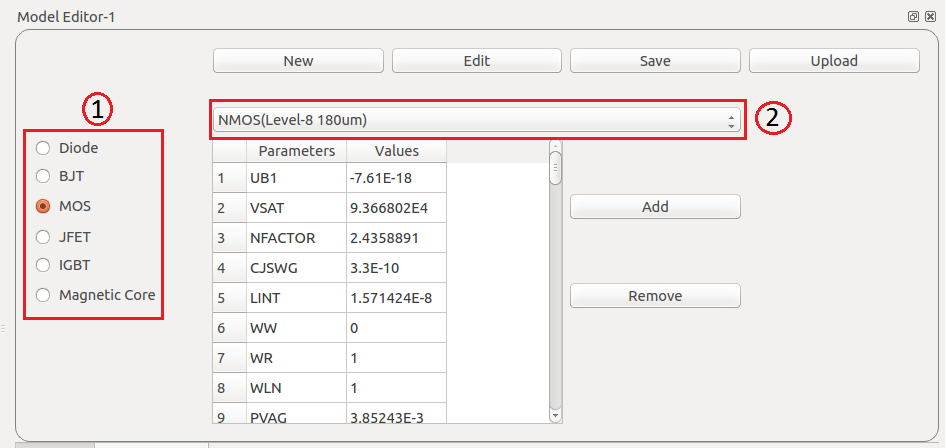
\includegraphics[width =\lgfig]{modelnew.png}
\caption{Choosing the Template Model Library }
\label{modelnew}
\end{figure}

\pagebreak

New parameters can be added or current parameters can be removed using {\tt ADD} and {\tt REMOVE} buttons. Also the values of parameters can be changed in the table. Adding and removing the parameters in library files is shown in the \figref{modeladd} and \figref{modelremove}

\begin{figure}
\centering
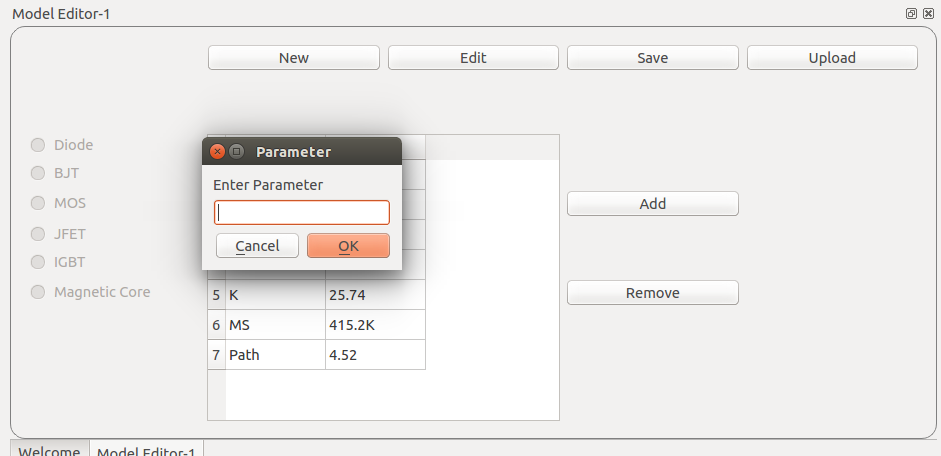
\includegraphics[width =\lgfig]{modeladd.png}
\caption{Adding the Parameter in a Library}
\label{modeladd}
\end{figure}

\begin{figure}
\centering
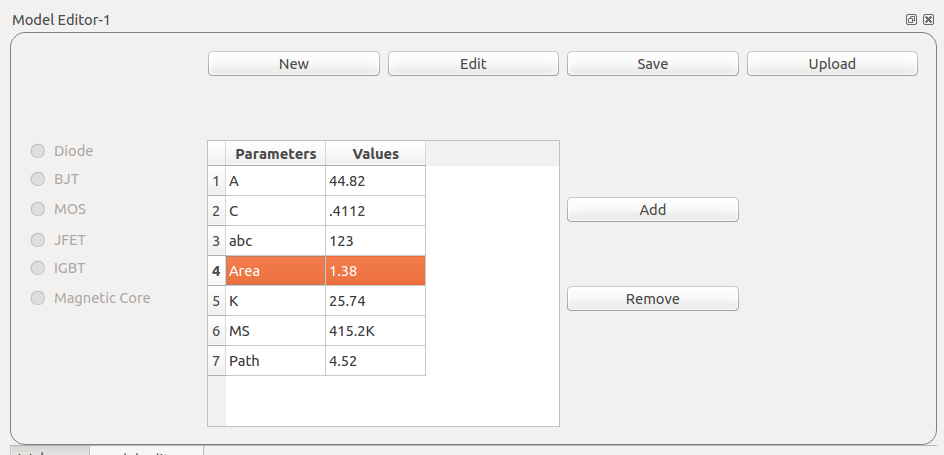
\includegraphics[width =\lgfig]{modelremove.png}
\caption{Removing a Parameter from a Library }
\label{modelremove}
\end{figure}

After the editing of the model library is done, the file can be saved by selecting the {\tt SAVE} button. These libraries are saved in the \textit{User Libraries} folder under \textit{deviceModelLibrary} directory.

\section{Editing Current Model Library}
The existing model library can be modified using {\tt EDIT} option. On clicking the {\tt EDIT} button the file dialog opens where all the library files are saved as shown in \figref{modeledit}. You can select the library you want to edit.
Once you are done with the editing, click on {\tt SAVE} button.

\begin{figure}
\centering
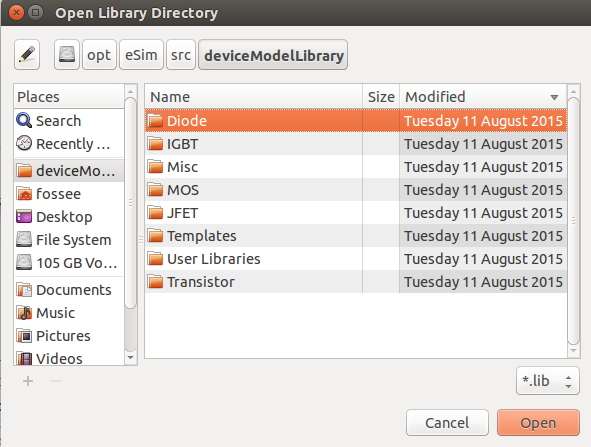
\includegraphics[width =\lgfig]{modeledit.png}
\caption{Editing Existing Model Library}
\label{modeledit}
\end{figure}

\section{Uploading external .lib file to eSim repository}
User can also upload external spice {\textbf{.model}} library files. These .model libraries can be downloaded online.  eSim directly cannot use the external .lib file. It has to be uploaded to eSim repository before using it in a circuit.
eSim provides the facility to upload library files using the {\textbf Upload} option in the {\textit 
{Model Editor}}. They are then converted into xml format, which can be easily modified from the eSim interface.
On clicking {\tt UPLOAD} button the library can be uploaded from any location. The model library will be saved with the name you have provided, in the \textit {User Libraries} folder of repository \textit{deviceModelLibrary}.
Example: You can download any model of Schottky diode from Spice website and save it as .lib extension on the system. Click on  {\tt UPLOAD} option and give the path. The lib file along with XML file is created in the {\tt eSim-<version>/library/deviceModeLibrary/UserLibraries} if you are using v2.0 \linebreak and above versions; otherwise \\
 {\tt eSim-<version>/src/deviceModeLibrary/UserLibraries} if you are using \linebreak versions lower than 2.0 \\. The uploaded library can be used for the existing part eSim\_Diode or the user can create a new model (part). Refer \chapref{chap8} on how to create a new part library model in eSim.
 % adds chapter 7
\chapter{SubCircuit Builder}
\label{chap8}
Subcircuit is a way to implement hierarchical modeling. Once a subcircuit for a compo-
nent is created, it can be used in other circuits. eSim provides an easy way to create
a subcircuit. The following \figref{subcircuit_mainwin} shows the window that is opened when the SubCircuit tool is chosen from the toolbar.
\begin{figure}[!htp]
\centering
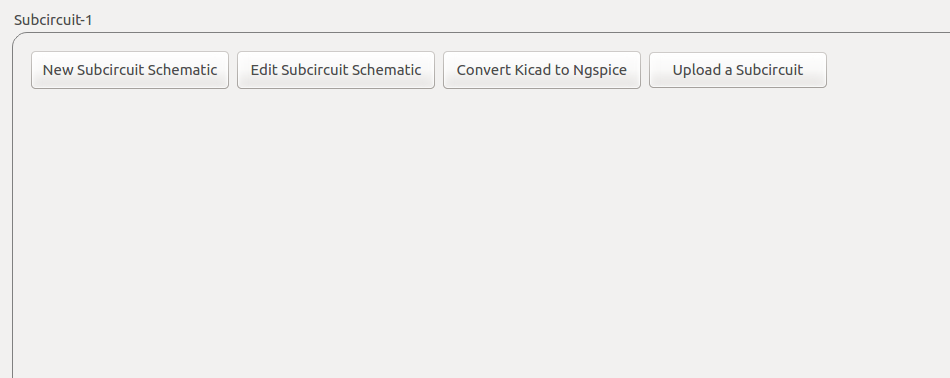
\includegraphics[width =\lgfig]{subcirciut_window.png}
\caption{Subcircuit Window}
\label{subcircuit_mainwin}
\end{figure}


\section{Creating a SubCircuit}
%Let us take an example of Half-adder circuit. To create a new sub circuit select the New Subcircuit Schematic.\figref{halfadder} shows the half-adder circuit. %and \figref{block} shows the block of the sub circuit included in the main circuit.
%\begin{figure}[!htp]
%\centering
%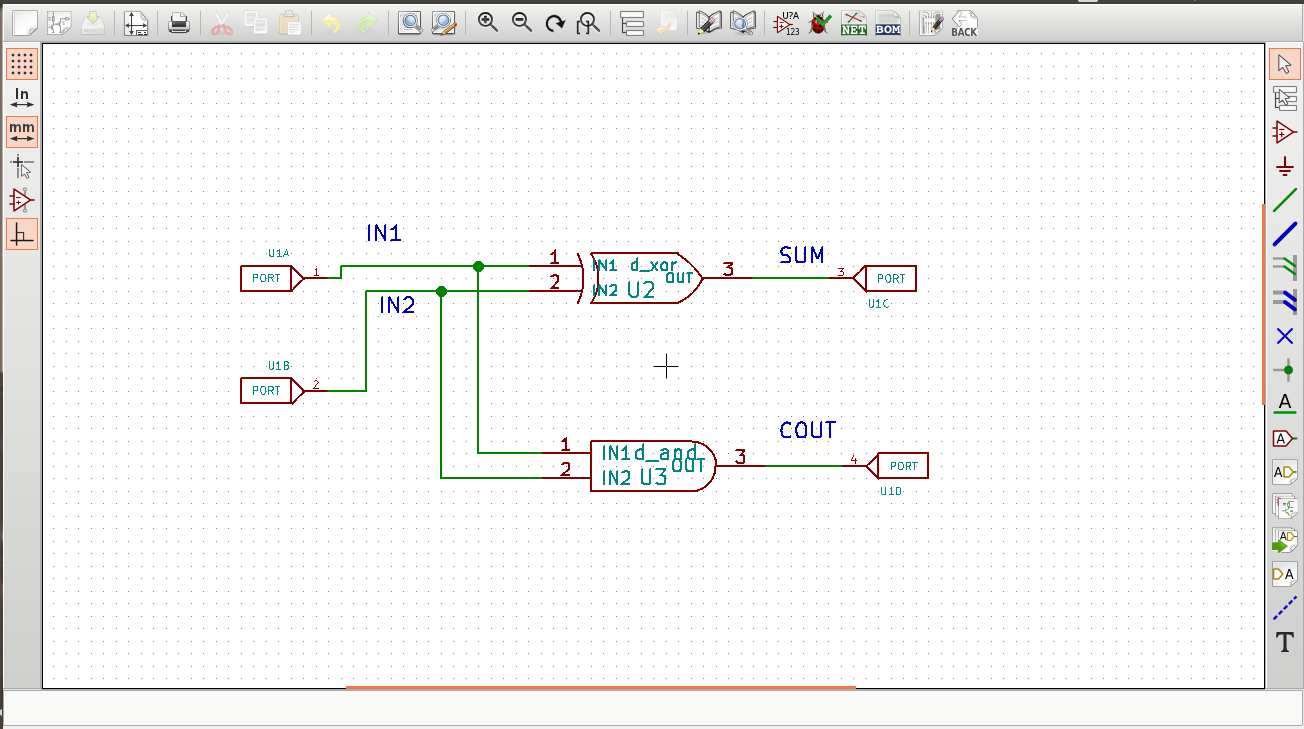
\includegraphics[width = 13cm, height= 7cm]{figures/half_adder.png}
%\caption{Half-Adder Sub-circuit }
%\label{halfadder}
%\end{figure}
%\textit {NOTE: All the input and output of the sub circuits are connected to the port component.}
%\begin{figure}
%\centering
%\includegraphics[width = 8cm, height= 7cm]{figures/halfadderblock.png}
%\caption{Half-Adder Sub-circuit Block }
%\label{block}
%\end{figure}
%After creating the schematic kicad netlist is generated as explained in section and convert kicad to Ngspice where cir.out and .sub files are generated.
%The number of input and output ports of the subcircuit is to matched with number of connections in the main circuit. eSim provides this validation of mapping of the sub circuit ports.
%Also the respective input and output ports can be checked by reading the .sub file.
The steps to create subcircuit are as follows.
\begin{itemize}

\item After opening the Subcircuit tool, click on {\tt New Subcircuit Schematic} button. It will ask the name of the subcircuit. Enter the name of subcircuit (without any spaces) and click {\tt OK} as shown in \figref{newsubcktschematic}.
      


        \begin{figure}[!htp]
            \centering
            \includegraphics[width =\lgfig]{newsubckt.png}
            \caption{New Sub circuit Window}
            \label{newsubcktschematic}
        \end{figure}

\item After clicking {\tt OK} button it will open KiCad schematic. Draw your circuit which will be later used as a subcircuit. e.g the \figref{createsubcktsch} shows the half adder circuit.
        
        \begin{figure}[!htp]
            \centering
            \includegraphics[width =\lgfig]{createsubcktsch.png}
            \caption{Inner circuit of the subcircuit}
            \label{createsubcktsch}
         \end{figure}



\item Once you complete the circuit, assign a PORT to each open node of your circuit which will be used to connect with the main circuit. The port should match with the number of input and output pin. The circuit will look like \figref{halfadder} after adding PORT to it. The PORT component can be found in the eSim\_Miscellaneous library as shown in \figref{port}. Select a different port for each node (input or output), the PORT has 26 such components named alphabetically as Unit A, Unit B to Unit Z, meaning you can create a subcircuit up-to 26 pins(input, output combined).
        
    
        \begin{figure}[!htp]
            \centering
            \includegraphics[width =\hgfig]{ha_sub.png}
            \caption{Half-Adder Subcircuit }
            \label{halfadder}
        \end{figure}


        \begin{figure}[!htp]
            \centering
            \includegraphics[width =\smfig]{misc_port_list.png}
            \caption{Selection of PORT component}
            \label{port}
        \end{figure}

    \item Next step is to save the schematic and generate KiCad netlist as explained in Chapter 5.

    \item To use this subcircuit in other schematics, create a block in the schematic editor by following steps given below as one should have a symbol corresponding to the newly created subcircuit that can be used in other schematics:
        \begin{enumerate}
            \item Go to library browser of the schematic editor. It is an "open book with a pencil in its middle" icon on the top toolbar.
            \item Select the Current Library as eSim\_Subckt shown in \figref{esimsubckt} 
                \begin{figure}[!htp]
                    \centering
                    \includegraphics[width =\smfig]{esim-subckt.png}
                    \caption{Selecting Working Library}
                    \label{esimsubckt}
                \end{figure}
            \pagebreak

        \item Click on create a new component from the top toolbar.
        \item Give the same name that was used for creating the new subcircuit's internal diagram, refer \figref{newsubcktschematic}.
        \item Choose designator as \textbf{X}. If any other reference designator other than X is used for \textbf{subcircuit}, your subcircuit will not be recognised during simulation.
        \item Similarly, reference designator are as follows for different types of components. D is for diode, Q is for transistors, J is for FET. The user needs to choose the appropriate reference based on the library in which they wish to add a model. 
            \begin{figure}[!htp]
                \centering         
                \includegraphics[width =\smfig]{subcktnewcomp.png}
                \caption{Creating New Component}
                \label{subcktnewcomp}
            \end{figure}


        \item Start drawing the subcircuit block by using the drawing tools from the right taskbar. Here we have used {\textitbf{\tt Add graphic rectangle to component body}}. You can start drawing with a point to point click on the editor.
        
        \item To add pins select {\textitbf {Add pins to components}} from the right taskbar. Give the {\tt Pin Name} as {\tt {IN1}} and {\tt{Pin Number as 1}}. The pin number has to match with the {\tt Port name}. Example Port A is mapped to pin 1. Select the {\textitbf{ Orientation}} as right or left accordingly. The {\textitbf{ Electrical Type}} has to be chosen as {\tt Input} for nodes which will act as Input in the subcircuit you are creating. Similar logic is for output nodes. We would recommend to declare the ports as either Input, Output or Passive.
        
        \item The final block of the subcircuit would look as shown in \figref{block}. Pins should be attached properly. Labels(Names to the PORTs) should be given such that it is intuitive and someone other than you should be able to understand and use that block with least amount of hassle.
        
        \item In order to save this file, press \textbf{Ctrl+S} keys and click \textbf{yes} for confirmation purposes. 
        
        \item Note : A good practice to retain this created subcircuit would be to take a backup of this library. To do that, click on \textbf{File} from the library editor window and select the \textbf{Save Current Library as} option. A location needs to be selected, please select \textbf{eSim-Workspace} as the location for storing this file and give relevant name e.g. \textbf{eSim-Subckt-backup}. Later other users can use this in their circuits.
        
        
                    \begin{figure}[!htp]
                        \centering
                        \includegraphics[width =\smfig]{halfadderblock.png}
                        \caption{Half-Adder Subcircuit Block}
                        \label{block}
                    \end{figure}
\end{enumerate}
        
\subsubsection{Specifying parameters for generating the \textbf{.sub} file }
\begin{enumerate}
\item A \textbf{.sub} file is nothing but textual representation that is passed to the simulator which essentially informs the simulator about the nodes, and behavior of the subcircuit block.
Remember the \figref{halfadder} circuit? It will be saved in a \textbf{.sub} file once we complete this process!
 \item Switch to the eSim main window and click on \textbf{Convert KiCad to Ngspice button} in the \textbf{subcircuit builder tool}. as shown in \figref{subcircuit_mainwin}
 \item You need not assign any values in the transient parameters section. \\
 Assign the values to any voltage or current sources present in your internal circuit, if any. \\
 Add the appropriate device libraries or subcircuit libraries if you have used any Device Models or  Subcircuits, if any. 
 \item Upon successful generation of the subcircuit file, an acknowledgement message will be displayed. To confirm, go to \\
 \large \textit{For Windows OS users} : \\
 \large {C:/FOSSEE/eSim/Library/SubcircuitLibrary if you are using v2.0 and above} \\
 \large C:/FOSSEE/eSim/src/SubcircuitLibrary if you are using versions \textbf{lower than 2.0} \\
 
 \large \textit{For Ubuntu Linux Users} \\
 ../eSim-2.0/Library/SubcircuitLibrary if you are using v2.0 and above \\
 ../eSim-1.1.3/src/SubcircuitLibrary if you are using versions \textbf{lower than 2.0} \\
 And make sure that the .sub file is present under the directory carrying the name of the subcircuit that you specified in step in \figref{newsubcktschematic}.
 
 \end{enumerate}

\end{itemize}

\section{Edit a Subcircuit}
The steps to edit a subcircuit are as follows.

\begin{itemize}
    \item After launching the Subcircuit tool, click on \textbf{Edit Subcircuit Schematic} button. It will open a dialog box where you can select any subcircuit for editing.
    \item After selecting the subcircuit it will open it in the schematic editor, where you can edit the subcircuit.
    \item Next step is to save the schematic and generate the .cir netlist.
    \item If you have edited the number of ports then you have to change the block exaplained in section {Creating a Subcircuit} accordingly.
\end {itemize}
    
{\textbf{Note}}:    
    
\begin{itemize}
\item User can also import or append the schematic of different projects in the current page using the \textit{Append Schematic Sheet} from the \textit{File} menu. This will import(copy) the schematic that user has defined to the current schematic editor page.
\item  User can also import the model in the part library editor page using the option \textit{Import Component} from the top toolbar.
\end{itemize}

\section{Upload subcircuit}
\begin{itemize}
    \item Using this feature, one can import an existing subcircuit file into eSim environment. You necessarily need not create the schematic for this.
    \item Download the required subcircuit's .sub file from many online resources/repositories. 
    \item Upload this file using the upload subcircuit feature.
    \item Upon uploading following checks will be made, and only and only if the checks are satisfied, the file will be uploaded. The checks are as following : \\
    1. The uploaded file should have the extension \textbf{.sub} \\
    2. The name of the file, say for example is \textbf{omega.sub}, then the content of the file must start with \textbf{.subckt omega} and end with \textbf{.ends omega}. \\
    Any line that starts with asterisk sign(*) is considered as a comment in these types of files. Hence, the file technically starts with \textbf{.subckt}.
    \item If above conditions are satisfied, then the file will be automatically placed in a folder that carries the same name as that of the .sub file will be created in ../SubcircuitLibrary/ directory.
    \item Once above steps are verified, proceed to create a block as shown in \figref{block} and name should be same as that of the corresponding .sub file uploaded earlier. Pins of this block should match the number of pins stated in the .sub file. \\
    NOTE: ONLY AND ONLY THE OUTER BLOCK NEEDS TO BE CREATED. INTERNAL CIRCUIT IS NOT REQUIRED IF YOU ARE USING THE UPLOAD FEATURE.
    
\end{itemize}
 % adds chapter 8
\chapter{NGHDL-Mixed Signal Simulation}
\label{chap9}
\thispagestyle{empty}


NGHDL feature facilitates creation of user-defined models for mixed-signal circuit simulation in eSim. By interfacing GHDL and Ngspice, we achieve mixed-signal simulation. Digital models are simulated using GHDL and XSpice engine of Ngspice. \\


%To access NGHDL click on the NGHDL button on the left pane of window as shown in figure \figref{screen3}:
%\pagebreak

\section{Introduction}

Ngspice supports mixed-signal simulation, i.e. it can simulate both digital and analog component. It defines a \texttt{model} which has the functionality of the circuit component, which can be used in the netlist.
For example you can create an \texttt{adder} model in Ngspice and use it in any circuit netlist of Ngspice. \\

However, it is not feasible to define complex digital models without a complete understanding of Ngspice and XSPICE architectures and is a time-consuming process. Also, most of the users are familiar with GHDL and can write the models using VHDL code with ease.
Hence, NGHDL provides an  interface to write VHDL code for a digital model and install it as model in Ngspice. So whenever Ngspice looks for that model, it will actually interface with VHDL code to get the result. \\

\begin{figure}[!htp]
\centering
\includegraphics[width = 13cm, height = 7cm]{./NGHDL/NGHDL_Overview.png}
\caption{Overview of NGHDL}
\label{overview}
\end{figure}
%description of Overview:
\figref{overview} shows the overview of NGHDL indicating its architecture at the abstract level. The values for the digital models present in the netlist are fetched from the GHDL side of the interface whereas the values of the analog part are fetched from Ngspice's spice3f5 engine. Digital and Analog components in \figref{overview} are connected to each other with the help of the hybrid ADC and DAC models provided by Ngspice. This helps in the signal level switching when simulation is performed. As analog signals are in continuous time domain and Digital signals are in discrete time domain, hybrid components help bridge the gap. More information on the parameters of ADC and DAC present in Appendix : D.

\pagebreak

\section{Digital Model creation using NGHDL}

%Description of User Flow of NGHDL

\begin{figure}[!htp]
\centering
\includegraphics[width = 13cm, height = 7cm]{./NGHDL/NGHDL_Flow.png}
\caption{User Flow for NGHDL}
\label{user_flow}
\end{figure}

\noindent \textbf{The steps to create digital models are given below}:

\begin{enumerate}
\item Click on NGHDL button on left side pane of main window, the Ngspice Digital Model Creator window will appear as shown in  \figref{screen3}
        \begin{figure}[!htp]
            \centering
            \includegraphics[height=10cm, width =\lgfig]{./NGHDL/screen3.png}
            \caption{NGHDL interface}
            \label{screen3}
        \end{figure}


\item Now browse and locate the VHDL file to upload. Select the VHDL file and click on the Upload button. This process will create Ngspice model and corresponding component drawing inside the KiCad library (eSim\_Nghdl.lib) of the VHDL block to be used in mixed-signal simulations. An acknowledgement message will appear upon sucessful processing of the VHDL code as shown in \figref{upload}. \\

        \begin{figure}[!htp]
            \centering
            \includegraphics[width =\smfig]{./NGHDL/screen4.png}
            \caption{Uploading of digital model}
            \label{upload}
         \end{figure}
         
Note : \texttt{"Add files"} option allow you to use a smaller entity / subpart / submodule to support the main VHDL file. That is, a digital model will be generated corresponding to that file that has been browsed. The file that has been \texttt{"added"} to Nghdl upload window will only be placed along with the model under model’s DUTghdl folder to support the model.

Hence, \texttt{"browsing"} one file and \texttt{"adding"} several files won’t create that many number of models, but only one model will be created corresponding to the browsed file.
\end{enumerate}

\section{Schematic Creation}
Steps for schematic creation are as follows:
\begin{enumerate}
\item Click on New Project icon to create a new project as shown in \figref{screen1}, be careful of the naming conventions.
%To access nghdl click on the NGHDL button on the left pane of window as shown in figure \figref{screen3}:

\begin{figure}[!htp]
\centering
\includegraphics[width = 13cm, height = 7cm]{./NGHDL/screen1.png}
\caption{Creation of a new project}
\label{screen1}
\end{figure}

\item After successful upload of the model using the VHDL code, you can create the schematic of your design by clicking on \texttt{Open Schematic} button on the left pane of the eSim window. Then go to \texttt{Preferences} option on top of the schematic editor window and click on \texttt{Component Libraries} to add the library eSim\_Nghdl.lib in KiCad. Following window will appear as shown in \figref{screen6}, where you will have to click on \textit {Add} button and select the \texttt{eSim\_Nghdl} library. Refer \figref{screen6} and \figref{screen7}. %%last sentence may not be required
    
        \begin{figure}[!htp]
            \centering
            \includegraphics[width =\smfig]{./NGHDL/screen6.png}
            \caption{Adding the digital model library in KiCad}
            \label{screen6}
        \end{figure}


        \begin{figure}[!htp]
            \centering
            \includegraphics[width =\smfig]{./NGHDL/screen7.png}
            \caption{Selection of library} %%this may not be required either
            \label{screen7}
        \end{figure}


    
    \pagebreak
    \item Next step is to locate the component in \texttt{eSim\_Nghdl} library as shown in \figref{screen9} and place it on the schematic editor as shown in \figref{screen10}.
        \begin{figure}[!htp]
            \centering
            \includegraphics[width =\smfig]{./NGHDL/screen9.png} %%Change this image
            \caption{Locating the component in library} 
            \label{screen9}
        \end{figure}


        \begin{figure}[!htp]
            \centering
            \includegraphics[width =\smfig]{./NGHDL/screen10.png}
            \caption{Placement of component on editor}
            \label{screen10}
        \end{figure}
\pagebreak

\item Now create the schematic as shown in \figref{screen14}, annotate, perform ERC, create the netlist and save the schematic by following the steps given in Chapter 5.
\begin{figure}[!htp]
            \centering
            \includegraphics[width =\hgfig]{./NGHDL/screen14.png}
            \caption{Example of an AND gate characteristics circuit}
            \label{screen14}
        \end{figure}

\item After creating the schematic, click on \texttt{KiCad-to-Ngspice converter} and select the type of analysis as transient as shown in \figref{screen15} and set the start, step and stop time as shown in \figref{screen16}
   \begin{figure}[!htp]
                \centering
                \includegraphics[width =\hgfig]{./NGHDL/screen15.png}
                \caption{Analysis Part I}
                \label{screen15}
            \end{figure}
           \begin{figure}[!htp]
            \centering
            \includegraphics[width =\hgfig]{./NGHDL/screen16.png}
            \caption{Analysis Part II}
            \label{screen16}
        \end{figure}
\pagebreak

\item Now click on \texttt{Source Details} and enter the values for Source v1 and source v2 as shown in figure \figref{val1} and \figref{val2}
\begin{figure}[!htp]
                \centering
                \includegraphics[width =\hgfig]{./NGHDL/val1.png}
                \caption{Value of Source v1}
                \label{val1}
            \end{figure}
           \begin{figure}[!htp]
            \centering
            \includegraphics[width =\hgfig]{./NGHDL/val2.png}
            \caption{Value of Source v2}
            \label{val2}
        \end{figure}

\item Now select the option \texttt{Ngspice Model}, window as shown in \figref{screen17} will appear. The values of the parameters listed can be changed per user's requirement. If you have used any semicnductor devices and Subcircuits in your design, then please specify the Spice models and subcircuits in the \texttt{Device Modeling} and \texttt{Subcircuits} tabs of the \texttt{KiCad-to-Ngspice converter} window.  After that click on \texttt{Convert} button. This step will create the simulation compatible netlist.
                    \begin{figure}[!htp]
                        \centering
                        \includegraphics[width =\hgfig]{./NGHDL/screen17.png} %Change the figure
                        \caption{Model Parameters}
                        \label{screen17}
                    \end{figure}
\item Now click on \texttt{Simulation} button, it will display the following windows as shown in \figref{screen19}. This is the Ngspice terminal and Python plot window.
\begin{figure}[!htp]
                        \centering
                        \includegraphics[width =\hgfig]{./NGHDL/screen19.png}
                        \caption{Simulation window}
                        \label{screen19}
                    \end{figure}
\pagebreak 
\item Now select the required nodes and click on \texttt {Plot} button. You can see the plots of input source v1, input source v2 and output as shown in \figref{plotv1}, \figref{plotv2}, and \figref{plotout} respectively.
\begin{figure}[!htp]
                        \centering
                        \includegraphics[width =\lgfig]{./NGHDL/plotv1.png}
                        \caption{Plot of Source V1}
                        \label{plotv1}
                    \end{figure}
\begin{figure}[!htp]
                        \centering
                        \includegraphics[width =\lgfig]{./NGHDL/plotv2.png}
                        \caption{Plot of source V2}
                        \label{plotv2}
                    \end{figure}
\begin{figure}[!htp]
                        \centering
                        \includegraphics[width =\lgfig]{./NGHDL/plotout.png}
                        \caption{Plot of output}
                        \label{plotout}
                    \end{figure}

        \pagebreak

\end{enumerate} % adds chapter 9
\chapter{OpenModelica}
\thispagestyle{empty}
\label{chap10}

\section {Introduction}
OpenModelica (OM) is an open source modeling and simulation tool based on
Modelica language. Modelica is an object oriented language. As a result, it has all the
features of an object oriented language such as inheritance. Models or circuits are
defined in the form of classes, with in which there are components, functions,
connection and placement information. The OM suite has the following major tools.

\subsection {OMEdit}
An IDE for modeling and simulation. It supports a lot of electrical components. It
has a good graphical interface to drag and drop components and create the circuit.
One can only do transient simulation using this interface. An attractive feature of
OMEdit is the plotting interface. All the parameters in the circuit like voltages and currents through each component,
parameters like frequency, delay etc. will be displayed as
a list, after simulation. The user can choose the variables to be plotted in an
interactive manner from this list. On choosing the variable to plot, it will be plotted
on the plot window. One can also create multiple plot windows.

\subsection {OMOptim}
An IDE for optimisation. It lists all the variables in the given model. One can choose
the variables to be optimised from the list. Multiple models can be loaded for a given
optimisation problem. One can do multi objective optimisations as well. It supports
various optimisation algorithms such as Particle Swarm Optimisation (PSO) and
Simulated Annealing (SA). The results are displayed graphically.

\section {OpenModelica in eSim}
The above two functionalities can be accessed through the {\tt Modelica Converter} and {\tt OM Optimisation} tools on the eSim left toolbar. The two examples given below illustrates how to use OpenModelica in eSim. 

\subsubsection {Low Pass Filter circuit} 
Let us now see how to simulate a low pass filter in OpenModelica.
\begin{enumerate}
\item Open the schematic and create the circuit as shown in \figref{lowpass}. 

\begin{figure}[h]
\centering
\includegraphics[width=\lgfig]{list_of_figures/1.png}
\caption{Circuit schematic: Low pass filter}
\label{lowpass}
\end{figure}

\item Create the KiCad netlist. Now the analysis and analysis parameters are given as shown in \figref{lowpass-analysis}. 

\begin{figure}[h]
\centering
\includegraphics[width=\lgfig]{list_of_figures/2.png}
\caption{Analysis parameters: Low pass filter}
\label{lowpass-analysis}
\end{figure}

\item The source details are given as in \figref{lowpass-source}. The generated KiCad netlist is then converted to ngspice compatible netlist.

\begin{figure}[h]
\centering
\includegraphics[width=\lgfig]{list_of_figures/3.png}
\caption{Source details: Low pass filter}
\label{lowpass-source}
\end{figure}

\item Simulate the ngspice netlist. The simulation curves are shown in \figref{lowpass-simulation}.

\begin{figure}[h]
\centering
\includegraphics[width=\lgfig]{list_of_figures/4.png}
\caption{Simulation: Low pass filter}
\label{lowpass-simulation}
\end{figure}

\item Now to use OpenModelica, click on {\tt Modelica Converter} in the bottom left of eSim left toolbar.{\textit Make sure you have OpenModelica installed in the system}. This converter converts the spice netlist to Modelica format. Click on the LPF in the left that is appended in OpenModelica main window. Make sure you are in text view to see the Modelica code as shown in \figref{om-convert} Figure shows that LPF circuit is being used as a model, the initialisation of sources and components are in the beginning followed by the connection information. n3, n0,n2 are the nodes.

\begin{figure}[h]
\centering
\includegraphics[width=\lgfig]{list_of_figures/5.png}
\caption{OpenModelica: Text view}
\label{om-convert}
\end{figure}

Default Modelica libary is used for electrical sources and components. This has to imported so that it can be used in the current circuit. This is available in the left side of main window. 

\item Click on Simulation Setup on the toolbar at the top. A window opens as shown in \figref{om-simsetup}. Give start and stop time. Click {\tt OK}.

\begin{figure}[h]
\centering
\includegraphics[width=\lgfig]{list_of_figures/6.png}
\caption{OpenModelica: Simulation setup}
\label{om-simsetup}
\end{figure}

\item A plotting window opens. Click on the node at the right to display the waveform. The window is shown in \figref{om-simulation}.

\begin{figure}[h]
\centering
\includegraphics[width=\lgfig]{list_of_figures/7.png}
\caption{OpenModelica: Simulation}
\label{om-simulation}
\end{figure}

\end{enumerate}

\subsection {OM Optimisation}

Now let us explore how to use OpenModelica for optimisation through an example. Find the value of resistance R2 that maximises the power dissipated through it for the circuit in \figref{optim-circuit}. This is an illustration of the Maximum Power Transfer Theorem. The power is maximum when R2 = R1, i.e., when R2 = 100. So maximum power would be Pmax = 0.0625. Let us now see the steps to be followed find the value of R2 using eSim.

\begin{figure}[h]
\centering
\includegraphics[width=\lgfig]{list_of_figures/8.png}
\caption{Circuit schematic for optimisation}
\label{optim-circuit}
\end{figure}

\begin{enumerate}
\item Follow all the steps as above and generate the Modelica model using the Ngspice to Modelica converter.

\item The objective function is $Power = i^2 \times R2$ . 
To define the objective function, the line $power := i^2 \times R1+ i^2 \times R2$  
is added under the keyword algorithm, in the Modelica model file.

\item Select {\tt OMOptim} from eSim left toolbar, in the displayed window click on {\tt New Project}. Then save the project. It is stored with an extension {\tt .min}. Now select {\tt Models} and then {\tt Load Modelica Library}. Now select {\tt Load mo file} under {\tt Models}. It will be added on the left. 

\item Click {\tt Problems} and then {\tt Optimisation}. Select the model to be optimised. \textit {Note that for optimising, that model has to be loaded in OpenModelica as stated before}. Clicking
blue turnover icon will display all the variables used in the model. Add details like optimsation variables and objective.

The OMOptim project for this problem is given in \figref{om-project}. Power is the objective function that has to be maximized. {\tt r2.R} is the variable that will be varied. {\tt r2.R} is limited between 0 and 1000.

\begin{figure}[h]
\centering
\includegraphics[width=\hgfig]{list_of_figures/9.png}
\caption{OMOptim project}
\label{om-project}
\end{figure}

\item Click on Parameters tab to select the type of algorithm and its parameters. In this example, the optimisation algorithm used is PSO (Particle Swarm Optimisation). The various parameter values given are as follows: population size as 50, Inertia factor as 1, Learning factor: alpha and beta as 2, Population saving frequency was 1. Iteration limit is also specified. Select the .mo file to be simulated from {\tt Files} tab. Click on {\tt Launch}. The results of optimisation for various values of Iteration Limit are given in \figref {table}.

\begin{figure}[h]
\centering
\includegraphics[width=\lgfig]{list_of_figures/10.png}
\caption{Optimisation values for various Iteration Limit }
\label{table}
\end{figure}

\item Depending on the type of algorithm, the time for optimisation varies. Optimised result is graphically displayed as shown in \figref {om-optimised}. 

\begin{figure}
\centering
\includegraphics[width=\hgfig]{list_of_figures/11.png}
\caption{Optimised value of resistance for maximum power }
\label{om-optimised}
\end{figure}

\end{enumerate}

 % adds chapter 10
\chapter{Solved Examples}
\thispagestyle{empty}
\label{chap11}

\section{Solved Examples}

%---------------RC circuit-------------------
\subsection{Basic RC Circuit}
\subsubsection{Problem Statement:} Plot the Input and Output Waveform of an RC circuit whose input voltage (Vs) is 50Hz, 3V peak to peak. The values of Resistor (R) and Capacitor(C) are $1k$ and $1uf$ respectively.
\subsubsection{Solution:}
\begin{itemize}
\item Creating a Project:
The new project is created by clicking the {\tt New} icon on the menubar. The name of the project is given in the pop up window as shown in \figref{rc1}.
\begin{figure}[!htp]
    \centering
    \includegraphics[width=\hgfig]{figures/rc1.png}
    %\includegraphics[width=\linewidth]{figures/rc1.png}
    \caption{Creating New Project}
    \label{rc1}
\end{figure}

\item Creating the Schematic:
To create the schematic, click the very first icon of the left toolbar as shown in the \figref{rc2}. This will open KiCad Eeschema.

\begin{figure}[!htp]
    \centering
    \includegraphics[width=\smfigp]{figures/rc2.png}
    %\includegraphics[width=\linewidth]{figures/rc2.png}
    \caption{Open Schematic Editor}
    \label{rc2}
\end{figure}

To create a schematic in KiCad, we need to place the required components. \figref{rc_component} shows the icon on the right toolbar which opens the component library.

\begin{figure}[!htp]
    \centering
    \includegraphics[width=\tnfig]{figures/rc_component.png}
    %\includegraphics[width=\linewidth]{figures/rc_component.png}
    \caption{Place Component Icon}
    \label{rc_component}
\end{figure}

\pagebreak

After all the required components of the simple RC circuit are placed, wiring is done using the {\tt Place Wire} option as shown in the \figref{rc_wire} 

\begin{figure}[!htp]
    \centering
    \includegraphics[width=\tnfig]{figures/rc_wire.png}
    %\includegraphics[width=\linewidth]{figures/rc_wire.png}
    \caption{Place Wire Icon}
    \label{rc_wire}
\end{figure}

Next step is {\tt ERC (Electric Rules Check)}. \figref{erc1} shows the icon for {\tt ERC}.

\begin{figure}[!htp]
    \centering
    \includegraphics[width=\lgfig]{figures/erc1.png}
    %\includegraphics[width=\linewidth]{figures/erc1.png}
    \caption{Electric Rules Check Icon}
    \label{erc1}
\end{figure}

\figref{rc_complete1} shows the RC circuit after connecting the components by wire.

\begin{figure}[!htp]
    \centering
    \includegraphics[width=\lgfig]{figures/rc_complete1.png}
    \caption{RC circuit}
    \label{rc_complete1}
\end{figure}

\pagebreak

After clicking the {\tt ERC} icon a window opens up. Click the {\tt Run} button to run rules check. The errors are listed in as shown in \figref{erc2}. This error is handled by adding {\tt Power Flag} as shown in \figref{rc_pwr}.

\begin{figure}[!htp]
    \centering
    \subfloat[ERC Run]{
        \includegraphics[width=\smfig]{figures/erc2.png}
    \label{erc2}} \hfill
    \subfloat[Power Flag]{
        \includegraphics[width= 5cm, height=5cm]{figures/rc_pwr.png}
    \label{rc_pwr}}
    \caption{ERC check and POWER FLAG}
\end{figure}

After adding the {\tt Power Flag} the completed RC circuit is shown in \figref{rc_schematic} and the netlist is generated as shown in \figref{rc_netlist}.


\begin{figure}[!htp]
    \centering
    \subfloat[Schematic of RC circuit]{
        \includegraphics[width=\smfig]{figures/rc_schematic.png}
    \label{rc_schematic}} \hfill
    \subfloat[Generating KiCad Netlist of RC circuit]{
        \includegraphics[width=\smfig]{figures/rc_netlistgeneration.png}
    \label{rc_netlist}}
    \caption{RC Schematic and Netlist Generation}
\end{figure}

\pagebreak
\item Convert KiCad to Ngspice:
To convert KiCad netlist of RC circuit to NgSpice compatible netlist click on KiCad to Ngspice icon as shown in \figref{rcki2ng}.

\begin{figure}[!htp]
\centering
\includegraphics[width=\tnfig]{figures/rc_ki2ng.png}
\caption{Convert KiCad to Ngspice Icon}
\label{rcki2ng}
\end{figure}

Now you can enter the type of analysis and source details as shown in \figref{rc_analysistab} and \figref{rc_sourcedetailstab} respectively.

\begin{figure}[!htp]
    \centering
    \subfloat[RC Analysis]{
        \includegraphics[width=\smfig]{figures/rc_analysistab.png}
    \label{rc_analysistab}} \hfill
    \subfloat[RC Source Details]{
        \includegraphics[width=\smfig]{figures/rc_sourcedetailstab.png}
    \label{rc_sourcedetailstab}}
    \caption{RC Analysis and Source Detail}
\end{figure}
The other tab will be empty as RC circuit do not use any Ngspice model, device library and subcircuit.

After entering the value, press the convert button. It will convert the netlist into Ngspice compatible netlist.

\pagebreak

\item Simulation:
To run Ngspice simulation click the simulation icon in the tool bar as shown in the \figref{rcplot}.
\begin{figure}[!htp]
\centering
\includegraphics[width=\tnfig]{figures/rc_plot.png}
\caption{Simulation Icon}
\label{rcplot}
\end{figure}

In eSim, there are two types of plot. First is normal Ngspice plot and second is interactive python plot as shown in \figref{rc_ngspiceplot} and \figref{rc_pythonplot} respectively.

\begin{figure}[!htp]
    \centering
    \subfloat[Ngspice Plot of RC]{
        \includegraphics[width=\lgfig]{figures/rc_ngspiceplot.png}
    \label{rc_ngspiceplot}}  \hfill
    \subfloat[Python Plot of RC]{
        \includegraphics[width=\lgfig]{figures/rc_pythonplot.png}
    \label{rc_pythonplot}}
    \caption{Ngspice and Interactive Python Plotting}
\end{figure}

In the interactive python plot you can select any node or branch to  plot voltage or current across it. Also it has the facility to plot basic functions across the node like addition, substraction, multiplication, division and v/s.  

\end{itemize}
%-----------------------Half Wave Rectifier---------------------------
\pagebreak

\subsection{Half Wave Rectifier}

\subsubsection{Problem Statement:} Plot the Input and Output Waveform of Half Wave Rectifier circuit where the input voltage (Vs) is 50Hz, 2V peak to peak. The value for Resistor (R) is 1k.

\subsubsection{Solution:}
The new project is created by clicking the {\tt New} icon on the menubar. The name of the project is given in the window shown in \figref{rc1}.

\begin{itemize}
\item Creating Schematic:
To create the schematic, click the very first icon of the left toolbar as shown in the \figref{rc2}. This will open KiCad Eeschema.\\

After the KiCad window is opened, to create a schematic we need to place the required components. \figref{rc_component} shows the icon on the 
right toolbar which opens the component library.\\

After all the required components of the simple Half Wave rectifier circuits are placed, wiring is done using the {\tt Place Wire} option as shown in the \figref{rc_wire}\\

Next step is {\tt ERC (Electric Rules Check)}. \figref{erc1} shows the icon for {\tt ERC}. After completing all the above steps the final Half Wave Rectifier schematic will look like \figref{hwr_schematic}.\\

\begin{figure}[!htp]
    \centering
    \includegraphics[width=\lgfig]{figures/hwr_schematic.png}
    \caption{Schematic of Half Wave Rectifier circuit}
    \label{hwr_schematic}
\end{figure}

\pagebreak

KiCad netlist is generated as shown in the \figref{hwr_netlistgeneration} \\

\begin{figure}[!htp]
    \centering
    \includegraphics[width=\lgfig]{figures/hwr_netlistgeneration.png}
    \caption{Half Wave Rectifier circuit Netlist Generation}
    \label{hwr_netlistgeneration}
\end{figure}

\item Convert KiCad to Ngspice: After creating KiCad netlist, click on the {\tt KiCad-Ngspice converter} button. This will open converter window where you can enter details of Analysis, Source values and Device library.

\begin{figure}[!htp]
    \centering
    \subfloat[Half Wave Rectifier Analysis]{
        \includegraphics[width=\smfig]{figures/hwr_analysistab.png}
    \label{hwr_analysistab}} \hfill
    \subfloat[Half Wave Rectifier Source Details]{
        \includegraphics[width=\smfig]{figures/hwr_sourcedetailstab.png}
    \label{hwr_sourcedetailstab}} \hfill
    \subfloat[Half Wave Rectifier Device Modeling]{
        \includegraphics[width=\smfig]{figures/hwr_devicemodelingtab.png}
    \label{hwr_devicemodelingtab}}
    \caption{Analysis, Source and Device Tab}
\end{figure}

Under device library you can add the library for diode used in the circuit. If you do not add any library it will take default Ngspice model.


\item Simulation: Once the KiCad-Ngspice converter runs successfully, you can run simulation by clicking the simulation button in the toolbar.
\begin{figure}[!htp]
    \centering
    \subfloat[Ngspice Plot of Half Wave Rectifier]{
        \includegraphics[width=\lgfig]{figures/hwr_ngspiceplot.png}
    \label{hwr_ngspiceplot}} \hfill
    \subfloat[Python Plot of Half Wave Rectifier]{
        \includegraphics[width=\lgfig]{figures/hwr_pythonplot.png}
    \label{hwr_pythonplot}}
    \caption{Half Wave Rectifier Simulation Output}
\end{figure}


\end{itemize}

\pagebreak
%-------------- Precision rectifier--------------------------------------

%\pagebreak

%\subsection{Precision Rectifier}
%\subsubsection{Problem Statement:} Plot the input and output waveform of the Precision Rectifier circuit where input voltage (Vs) is $50Hz$ , $3V$ peak to peak.

%\subsubsection{Solution:}
%The new project is created by clicking the {\tt New} icon on the menubar. The name of the project is given as shown in the \figref{rc1}.

%\begin{itemize}
%\item Creating Schematic:
%To create the schematic, click the very first icon of the left toolbar as shown in the \figref{rc2}. This will open KiCad Eeschema.\\
%After the KiCad window is opened, to create a schematic we need to place the required components. \figref{rc_component} shows the icon on the right toolbar which opens the component library.\\
%After all the required components of the precision rectifier circuit are placed, wiring is done using the {\tt Place Wire} option as shown in the \figref{rc_wire}.\\
%Next step is {\tt ERC (Electric Rules Check)}. \figref{erc1} shows the icon for {\tt ERC}.
%The \figref{pr_schematic} shows the complete Precision Rectifier schematic after removing the errors.

%\begin{figure}[!htp]
%\centering
%\includegraphics[width=\hgfig]{figures/pr_schematic.png}
%\caption{Schematic of Precision Rectifier circuit}
%\label{pr_schematic}
%\end{figure}

%The KiCad netlist is generated as shown in \figref{pr_netlistgeneration}.\\

%\begin{figure}[!htp]
%    \centering
%    \includegraphics[width=\lgfig]{figures/pr_netlistgeneration.png}
%    \caption{Precision Rectifier circuit Netlist Generation}
%    \label{pr_netlistgeneration}
%\end{figure}

%\pagebreak

%\item Convert KiCad to Ngspice: After creating KiCad netlist, click on KiCad-Ngspice converter button.\\ 

%    This will open converter window where you can enter details of Analysis, Source values, Device library and Subcircuit.

%\begin{figure}[!htp]
%   \centering
%    \subfloat[Precision Rectifier Analysis]{
%        \includegraphics[width=\smfig]{figures/pr_analysistab.png}
%    \label{pr_analysistab}} \hfill
%    \subfloat[Precision Rectifier Source Details]{
%        \includegraphics[width=\smfig]{figures/pr_sourcedetailstab.png}
%    \label{pr_sourcedetailstab}} \vfill
%    \subfloat[Precision Rectifier Device Modeling]{
%        \includegraphics[width=\smfig]{figures/pr_devicemodelingtab.png}
%    \label{pr_devicemodelingtab}}\hfill
%    \subfloat[Precision Rectifier Subcircuit]{
%        \includegraphics[width=\smfig]{figures/pr_subcircuitstab.png}
%    \label{pr_subcircuitstab}}
%    \caption{Analysis, Source, Device library and Subcircuit tab}
%\end{figure}

%Under device library you can add the library for the diode used in the circuit. If you do not add any library it will take default Ngspice 
%model for diode.\\

%Under subcircuit tab you have to add the subciruit used in your circuit. If you forget to add subcircuit it will throw an error.


%\pagebreak
%\item Simulation: Once the KiCad-Ngspice converter runs successfully, you can run the simulation by clicking the simulation button in the toolbar.
%\begin{figure}[!htp]
%    \centering
%    \subfloat[Ngspice Plot of Precision Rectifier]{
%        \includegraphics[width=\lgfig]{figures/pr_ngspiceplot.png}
%    \label{pr_ngspiceplot}} \hfill
%    \subfloat[Python Plot of Precision Rectifier]{
%        \includegraphics[width=\lgfig]{figures/pr_pythonplot.png}
%    \label{pr_pythonplot}}
%    \caption{Precision Rectifier Simulation Output}
%\end{figure}

%\end{itemize}

%-------------- Inverting Amplifier--------------------------------------

\pagebreak
\subsection{Inverting Amplifier}
\subsubsection{Problem Statement:}
Plot the Input and Output Waveform of Inverting Amplifier circuit where the input voltage (Vs) is $50Hz$, $2V$ peak to peak and gain is 2.
\subsubsection{Solution:}

\begin{itemize}
\item Creating Schematic:
To create the schematic, click the very first icon of the left toolbar as shown in the \figref{rc2}. This will open KiCad Eeschema.\\
After the KiCad window is opened, to create a schematic we need to place the required components. \figref{rc_component} shows the icon on the right toolbar which opens the component library.\\
After all the required components of the inverting amplifier circuit are placed, wiring is done using the {\tt Place Wire} option as shown in the \figref{rc_wire}.\\
Next step is {\tt ERC (Electric Rules Check)}. \figref{erc1} shows the icon for {\tt ERC}.

The \figref{ia_schematic} shows the complete Precision Rectifier schematic after removing the errors.

\begin{figure}[!htp]
    \centering
    \includegraphics[width=\hgfig]{figures/ia_schematic.png}
    \caption{Schematic of Inverting Amplifier circuit}
    \label{ia_schematic}
\end{figure}

The KiCad netlist is generated as shown in \figref{ia_netlistgeneration}.\\
\begin{figure}[!htp]
    \centering
    \includegraphics[width=\lgfig]{figures/ia_netlistgeneration.png}
    \caption{Inverting Amplifier circuit Netlist Generation}
    \label{ia_netlistgeneration}
\end{figure}


\item Convert KiCad to Ngspice:
After creating KiCad netlist, click on KiCad-Ngspice converter button.\\

This will open converter window where you can enter details of Analysis, Source values, Device library and Subcircuit.

Subcircuit of Op-Amp is shown in \figref{ia_sub}
    \begin{figure}[!htp]
        \centering
        \subfloat[Inverting Amplifier Analysis]{
            \includegraphics[width=\smfig]{figures/ia_analysistab.png}
        \label{ia_analysistab}} \hfill
        \subfloat[Inverting Amplifier Source Details]{
            \includegraphics[width=\smfig]{figures/ia_sourcedetailstab.png}
        \label{ia_sourcedetailstab}} \vfill
        \subfloat[Inverting Amplifier Subcircuit]{
            \includegraphics[width=\smfig]{figures/ia_subcircuitstab.png}
        \label{ia_subcircuitstab}}\hfill
        \subfloat[Sub-Circuit of Op-Amp]{
            \includegraphics[width=\lgfig]{figures/ia_sub.png}
        \label{ia_sub}}
        \caption{Analysis, Source, and Subcircuit tab}
    \end{figure}

\pagebreak
Under subcircuit tab you have to add the subciruit used in your circuit. If you forget to add subcircuit, it will throw an error.\\


\item Simulation: Once the KiCad-Ngspice converter runs successfully, you can run simulation by clicking the simulation button in the toolbar.
\begin{figure}
    \centering
    \subfloat[Inverting Amplifier Ngspice Plot]{
        \includegraphics[width=\lgfig]{figures/ia_ngspiceplot.png}
    \label{ia_ngspiceplot}}\vfill
    \subfloat[Inverting Amplifier Python Plot]{
        \includegraphics[width=\lgfig]{figures/ia_pythonplot.png}
    \label{ia_pythonplot}}
    \caption{Inverting Amplifier Simulation Output}
\end{figure}



\end{itemize}

%-------------------------Half Adder------------------------------------------

\pagebreak

\subsection{Half Adder}

\subsubsection{Problem Statement:}  Plot the Input and Output Waveform of Half Adder circuit.

\subsubsection{Solution:}

\begin{itemize}

\item Creating Schematic:  To create the schematic, click the very first icon of the left toolbar as shown in the \figref{rc2}. This will open KiCad Eeschema.\\
After the KiCad window is opened, to create a schematic we need to place the required components. \figref{rc_component} shows the icon on the right toolbar which opens the component library.\\
After all the required components of the Half Adder circuit are placed, wiring is done using the {\tt Place Wire} option as shown in the \figref{rc_wire}.\\
Next step is {\tt ERC (Electric Rules Check)}. \figref{erc1} shows the icon for {\tt ERC}.

The \figref{ha_schematic} shows the complete Half Adder schematic after removing the errors.
\begin{figure}[!htp]
    \centering
    \includegraphics[width=\hgfig]{figures/ha_schematic.png}
    \caption{Schematic of Half Adder circuit}
    \label{ha_schematic}
\end{figure}

The KiCad netlist is generated as shown in \figref{ha_netlistgeneration}.\\
\begin{figure}[!htp]
    \centering
    \includegraphics[width=\lgfig]{figures/ha_netlistgeneration.png}
    \caption{Half Adder circuit Netlist Generation}
    \label{ha_netlistgeneration}
\end{figure}

\pagebreak

\item Convert KiCad to Ngspice:
After creating KiCad netlist click on KiCad-Ngspice converter button.\\

This will open converter window where you can enter details of Analysis, Source values, Ngspice model and Subcircuit.

\begin{figure}[!htp]
    \centering
    \subfloat[Half Adder Analysis]{
        \includegraphics[width=\smfig]{figures/ha_analysistab.png}
    \label{ha_analysistab}} \hfill
    \subfloat[Half Adder Source Details]{
        \includegraphics[width=\smfig]{figures/ha_sourcedetailstab.png}
    \label{ha_sourcedetailstab}} \vfill
    \subfloat[Half Adder Ngspice Model]{
        \includegraphics[width=\smfig]{figures/ha_ngspicemodeltab.png}
    \label{ha_ngspicemodeltab}} \hfill
    \subfloat[Half Adder Subcircuit Model]{
        \includegraphics[width=\smfig]{figures/ha_subcircuitstab.png}
    \label{ha_subcircuitstab}}
    \caption{Analysis, Source, Ngspice Model and Subcircuit tab}
\end{figure}

Subcircuit of Half Adder in \figref{ha_sub}
\begin{figure}[!htp]
    \centering
    \includegraphics[width=\lgfig]{figures/ha_sub.png}
    \caption{Half Adder Subcircuit}
    \label{ha_sub}
\end{figure}

\pagebreak

\item Simulation: Once the KiCad-Ngspice converter runs successfully, you can run simulation by clicking the simulation button in the toolbar.
    \begin{figure}[!htp]
    \centering
    \subfloat[Half Adder Ngspice Plot]{
        \includegraphics[width=\lgfig]{figures/ha_ngspiceplot.png}
    \label{ha_ngspiceplot}} \hfill
    \subfloat[Half Adder Python Plot]{
        \includegraphics[width=\lgfig]{figures/ha_pythonplot.png}
    \label{ha_pythonplot}}
    \caption{Half Adder Simulation Output}
\end{figure}

\end{itemize}


%-------------------------Full Wave Rectifier using SCR------------------------------------------


\pagebreak

\subsection{Full Wave Rectifier using SCR}

\subsubsection{Problem Statement:}  Plot the Input and Output Waveform of Full Wave Rectifier using SCR.

\subsubsection{Solution:}

\begin{itemize}

\item Creating Schematic:  To create the schematic, click the very first icon of the left toolbar as shown in the \figref{rc2}. This will open KiCad Eeschema.\\
After the KiCad window is opened, to create a schematic we need to place the required components. \figref{rc_component} shows the icon on the right toolbar which opens the component library.\\
After all the required components of the Full Wave Rectifier using SCR circuit are placed, wiring is done using the {\tt Place Wire} option as shown in the \figref{rc_wire}.\\
Next step is {\tt ERC (Electric Rules Check)}. \figref{erc1} shows the icon for {\tt ERC}.

The \figref{fwrscr_schematic} shows the complete Rectifier circuit using SCR after removing the errors.
\begin{figure}[!htp]
    \centering
    \includegraphics[width=\hgfig]{figures/fwrscr_schematic.png}
    \caption{Schematic of Full Wave Rectifier using SCR}
    \label{fwrscr_schematic}
\end{figure}

The KiCad netlist is generated as shown in \figref{fwrscr_netlistgeneration}.\\
\begin{figure}[!htp]
    \centering
    \includegraphics[width=\lgfig]{figures/fwrscr_netlistgeneration.png}
    \caption{Full Wave Rectifier using SCR Netlist Generation}
    \label{fwrscr_netlistgeneration}
\end{figure}

\pagebreak

\item Convert KiCad to Ngspice:
After creating KiCad netlist click on KiCad-Ngspice converter button.\\

This will open converter window where you can enter details of Analysis, Source values, Ngspice model and Subcircuit.

\begin{figure}[!htp]
    \centering
    \subfloat[Full Wave Rectifier using SCR Analysis]{
        \includegraphics[width=\smfig]{figures/fwrscr_analysistab.png}
    \label{fwrscr_analysistab}} \hfill
    \subfloat[Full Wave Rectifier using SCR Source Details]{
        \includegraphics[width=\smfig]{figures/fwrscr_sourcedetailstab.png}
    \label{fwrscr_sourcedetailstab}} \vfill
    \subfloat[Full Wave Rectifier using SCR Subcircuit Model]{
        \includegraphics[width=\smfig]{figures/fwrscr_subcircuitstab.png}
    \label{fwrscr_subcircuitstab}}
    \caption{Analysis, Source and Subcircuit tab}
\end{figure}

Subcircuit of SCR in \figref{scr_sub}
\begin{figure}[!htp]
    \centering
    \includegraphics[width=\lgfig]{figures/scr_sub.png}
    \caption{SCR Subcircuit}
    \label{scr_sub}
\end{figure}

\pagebreak

\item Simulation: Once the KiCad-Ngspice converter runs successfully, you can run simulation by clicking the simulation button in the toolbar.
    \begin{figure}[!htp]
    \centering
    \subfloat[Full Wave Rectifier using SCR Ngspice Plot]{
        \includegraphics[width=\lgfig]{figures/fwrscr_ngspiceplot.png}
    \label{fwrscr_ngspiceplot}} \hfill
    \subfloat[Full Wave Rectifier using SCR Python Plot]{
        \includegraphics[width=\lgfig]{figures/fwrscr_pythonplot.png}
    \label{fwrscr_pythonplot}}
    \caption{Full Wave Rectifier using SCR Simulation Output}
\end{figure}

\end{itemize}


%-------------------------Oscillator------------------------------------------
\pagebreak

\subsection{Oscillator Circuit}

\subsubsection{Problem Statement:} Plot the Oscillation Waveforms for Phase Shift Oscillator circuit.

\subsubsection{Solution:}
The new project is created by clicking the {\tt New} icon on the menubar. The name of the project is given in the window shown in \figref{rc1}.

\begin{itemize}
\item Creating Schematic:
To create the schematic, click the very first icon of the left toolbar as shown in the \figref{rc2}. This will open KiCad Eeschema.\\

After the KiCad window is opened, to create a schematic we need to place the required components. \figref{rc_component} shows the icon on the 
right toolbar which opens the component library.\\

After all the required components of the Oscillator circuits are placed, wiring is done using the {\tt Place Wire} option as shown in the \figref{rc_wire}\\sss

Next step is {\tt ERC (Electric Rules Check)}. \figref{erc1} shows the icon for {\tt ERC}. After completing all the above steps the Oscillator schematic will look like \figref{osc_schematic}.\\

\begin{figure}[!htp]
    \centering
    \includegraphics[width=\lgfig]{figures/osc_schematic.png}
    \caption{Schematic of Phase Shift Oscillator circuit}
    \label{osc_schematic}
\end{figure}

\pagebreak

KiCad netlist is generated as shown in the \figref{osc_netlistgeneration} \\

\begin{figure}[!htp]
    \centering
    \includegraphics[width=\lgfig]{figures/osc_netlistgeneration.png}
    \caption{Phase Shift Oscillator circuit Netlist Generation}
    \label{osc_netlistgeneration}
\end{figure}

\item Convert KiCad to Ngspice: After creating KiCad netlist, click on the {\tt KiCad-Ngspice converter} button. This will open converter window where you can enter details of Analysis, Source values and Device library.

\begin{figure}[!htp]
    \centering
    \subfloat[Phase Shift Oscillator Analysis]{
        \includegraphics[width=\smfig]{figures/osc_analysistab.png}
    \label{osc_analysistab}} \hfill
    \subfloat[Phase Shift Oscillator Details]{
        \includegraphics[width=\smfig]{figures/osc_sourcedetailstab.png}
    \label{osc_sourcedetailstab}} \hfill
    \subfloat[Phase Shift Oscillator Device Modeling]{
        \includegraphics[width=\smfig]{figures/osc_devicemodelingtab.png}
    \label{osc_devicemodelingtab}}
    \caption{Analysis, Source and Device Tab}
\end{figure}

Under device library you can add the library for diode used in the circuit. If you do not add any library it will take default Ngspice model.


\item Simulation: Once the KiCad-Ngspice converter runs successfully, you can run simulation by clicking the simulation button in the toolbar.
\begin{figure}[!htp]
    \centering
    \subfloat[Ngspice Plot of Phase Shift Oscillator]{
        \includegraphics[width=\lgfig]{figures/osc_ngspiceplot.png}
    \label{osc_ngspiceplot}} \hfill
    \subfloat[Python Plot of Phase Shift Oscillator]{
        \includegraphics[width=\lgfig]{figures/osc_pythonplot.png}
    \label{osc_pythonplot}}
    \caption{Phase Shift Oscillator Simulation Output}
\end{figure}


\end{itemize}

%-------------------------BJT CB Characteristics------------------------------------------

\pagebreak

\subsection{Characteristics of BJT in Common Base Configuration}

\subsubsection{Problem Statement:} Plot Characteristics of BJT in Common Base Configuration.

\subsubsection{Solution:}
The new project is created by clicking the {\tt New} icon on the menubar. The name of the project is given in the window shown in \figref{rc1}.

\begin{itemize}
\item Creating Schematic:
To create the schematic, click the very first icon of the left toolbar as shown in the \figref{rc2}. This will open KiCad Eeschema.\\

After the KiCad window is opened, to create a schematic we need to place the required components. \figref{rc_component} shows the icon on the 
right toolbar which opens the component library.\\

After all the required components of the simple Half Wave rectifier circuits are placed, wiring is done using the {\tt Place Wire} option as shown in the \figref{rc_wire}\\

Next step is {\tt ERC (Electric Rules Check)}. \figref{erc1} shows the icon for {\tt ERC}. After completing all the above steps the BJT in CB Configuration schematic will look like \figref{cb_schematic}.\\

\begin{figure}[!htp]
    \centering
    \includegraphics[width=\lgfig]{figures/cb_schematic.png}
    \caption{Schematic of BJT in CB Configuration circuit}
    \label{cb_schematic}
\end{figure}

\pagebreak

KiCad netlist is generated as shown in the \figref{cb_netlistgeneration} \\

\begin{figure}[!htp]
    \centering
    \includegraphics[width=\lgfig]{figures/cb_netlistgeneration.png}
    \caption{BJT in CB Configuration circuit Netlist Generation}
    \label{cb_netlistgeneration}
\end{figure}

\item Convert KiCad to Ngspice: After creating KiCad netlist, click on the {\tt KiCad-Ngspice converter} button. This will open converter window where you can enter details of Analysis, Source values and Device library.

\begin{figure}[!htp]
    \centering
    \subfloat[BJT in CB Configuration Analysis]{
        \includegraphics[width=\smfig]{figures/cb_analysistab.png}
    \label{cb_analysistab}} \hfill
    \subfloat[BJT in CB Configuration Source Details]{
        \includegraphics[width=\smfig]{figures/cb_sourcedetailstab.png}
    \label{cb_sourcedetailstab}} \hfill
    \subfloat[BJT in CB Configuration Device Modeling]{
        \includegraphics[width=\smfig]{figures/cb_devicemodelingtab.png}
    \label{cb_devicemodelingtab}}
    \caption{Analysis, Source and Device Tab}
\end{figure}

Under device library you can add the library for diode used in the circuit. If you do not add any library it will take default Ngspice model.


\item Simulation: Once the KiCad-Ngspice converter runs successfully, you can run simulation by clicking the simulation button in the toolbar.
\begin{figure}[!htp]
    \centering
    \subfloat[Ngspice Plot of BJT in CB Configuration]{
        \includegraphics[width=\lgfig]{figures/cb_ngspiceplot.png}
    \label{cb_ngspiceplot}} \hfill
    \subfloat[Python Plot of BJT in CB Configuration]{
        \includegraphics[width=\lgfig]{figures/cb_pythonplot.png}
    \label{cb_pythonplot}}
    \caption{BJT in CB Configuration Simulation Output}
\end{figure}


\end{itemize}
 % adds chapter 11
\chapter{PCB Design}
\thispagestyle{empty}
\label{chap12}

Printed Circuit Board (PCB) \index{PCB} design is an important
step in electronic system design. Every component of the circuit
needs to be placed and connections routed to minimise delay and
area. Each component has an associated footprint. Footprint refers to
the physical layout of a component that is required to mount it on the
PCB. PCB design involves associating footprints to all components, placing them appropriately to
minimise wire length and area, connecting the footprints using
tracks or vias and finally extracting the required files needed for
printing the PCB. Let us see the steps to design PCB using eSim. 

\section{Schematic creation for PCB design}
In \chapref{chap5}, we have seen the differences between schematic for
simulation and schematic for PCB design. Let us design a PCB Layout for a 'constant 5V DC supply'  circuit named as \texttt{7805VoltageRegulator}. First, we will simulate the circuit. Refer to \figref{pcbschfin} for the schematic used for simulation. After satisfying simulation results, we will move to PCB design. For this, we will remove the Source(s), Probes (plot\_v , plot\_db etc.), and global labels connected \texttt{solely} for the purpose of viewing simulation plots conveniently. \\  Connectors are the physical components that are used to interface/connect the board to external peripherals or sources.

\begin{figure}
\centering
\includegraphics[width=\lgfig]{NGHDL/pcbschinitial.png}
\caption{Schematic for simulation of the constant 5V DC supply circuit}
\label{pcbschfin}
\end{figure}
 
%Create the circuit schematic as shown in \figref{pcbschfin}. The two pin female
%connector (\texttt{Conn\_01x02\_Female}) can be placed from the Eeschema's \texttt {Conn} library. Do the annotation and
%test for ERC.  Refer to \chapref{chap5} to know more about
%basic steps in schematic creation. 


\subsection{Removing components required for simulation from the schematic}
\begin{itemsize}
\item We will remove the components which were placed for simulation purpose only.
\item Components that will be placed on the board need to be added in the schematic.
\item Modify the circuit schematic as shown in \figref{pcbschconn}. The two pin female connector (\texttt{Conn\_01x02\_Female}) is placed for the taking the 5V output supply meanwhile a 2 pin Screw Terminal (\textt{Screw\_Terminal\_01x02}) is used to transmit the input signal on board. Do the annotation and test for ERC.  Refer to \chapref{chap5} to know more about basic steps in schematic creation. 
\begin{figure}
\centering
\includegraphics[width=\lgfig]{NGHDL/pcbschwithconn.png}
\caption{Schematic after adding connectors and removing the probes and sources.}
\label{pcbschconn}
\end{figure}
\end{itemsize}

\subsection{Mapping of components using Cvpcb}
%\index{Footprints!mapping} \index{Footprint Editor}
\index{Component!footprint!mapping}

\item Once the schematic for PCB Design is created, one needs to map each component
in the schematic to the appropriate footprint. The tool \texttt{Cvpcb} is
used for this.
\item Cvpcb can be launched by clicking the icon \texttt{Run Cvpcb to associate footprints and components} in Eeschema or by going under the \textt{Tools} menu and selecting \texttt{Assign Component Footprint} option. 

\subsection{Familiarising with Cvpcb Window}
\index{Cvpcb}
\begin{itemsize}
\item I. When one opens \texttt{Cvpcb} after annotating and running ERC on the schematic intended for PCB Design a window as shown in \figref{cvpcb} will be obtained. The Toolbar for using Cvpcb will be available in the top-most left corner.
\begin{figure}
\centering
\includegraphics[width=\lgfig]{NGHDL/cvpcb_unassigned.png}
\caption{Cvpcb window}
\label{cvpcb}
\end{figure}
\item II. The left pane has a list of all footprint libraries in the database.
\item III. The middle pane displays the list of components present in the schematic and if any footprint is assigned/associated to them.
\item IV. The right pane has a list of available footprints for each component depending upon how of libraries.
\end{itemsize}



\subsubsection{ Cvpcb Toolbar}
Some of the important tools in the toolbar are shown in
\figref{tb_fe}. They are explained below (Order of operation should ideally be from RIGHT to LEFT):
\begin{figure}
\centering
\includegraphics[width=\hgfig]{tb_fe.png}
\caption{Cvpcb Toolbar}
\label{tb_fe}
\end{figure}
\begin{compactenum}
\item Filter footprints list by library : We recommend the use of only this as a filtering method if you are completely new to eSim and/or PCB Design as it narrows down footprints based on libraries of the type of the component. When a filter is selected, it's icon will be highlighted in light red color as seen in \figref{tb_fe}.
\item Filter footprints list by pin count : This will filter the footprints based on number of pins the footprint has. This can be used to narrow down your search after sorting footprints by their library type.
\item Filter footprints list by keyword - This filters the footprints in the database based on keywords.
\item Automatic footprint association - Perform footprint association
  for each component automatically. Footprints will be selected from
  the list of footprints available.\\
  Note: This method of association is not recommended at all.
\item Delete all associations - Delete all the footprint associations made. This will erase all your association till now so be very careful in selecting this.
 \item Select next unlinked component: Using this you can go to the next component in the list of components for associating a footprint.
 \item Select previous unlinked component: Using this you can go to the previous component in the list of components for associating a footprint.
\item View selected footprint - View the selected footprint in 2D. See \secref{viewfp} for more details. \\
  Before clicking on this, make sure that a footprint is selected. Order of this operation should be
  \\ 1. Selection of footprint library from the left-most pane 
  \\ 2. Selecting a footprint from the right-most pane
  \\ 3. Click on \textt{View selected footprint}
\item Edit footprint library table - One should familiarize themselves with Cvpcb first and then only choose to use this. This impacts the footprints that you can choose, so be careful before making any severe changes.
\item Save netlist and footprint files - Save the netlist and the
  footprints that are associated with it. One ought to save the association after having assigned proper footprints to all the components.
\end{compactenum}

\subsection{Viewing footprints in 2D and 3D}
\index{Footprints!view!2D}
\index{Footprints!view!3D}
\label{viewfp}
\item To view a footprint in 2D, select the component for which you wish to view the available footprints, then select the library from left-most pane and now from the right pane and click on the desired footprint and click on \texttt{View selected footprint} from the menu bar. 
Let us view a footprint for \texttt{C1} from the \texttt{Capacitors\_THT} footprint library. Choose C1 from the middle pane as shown, click on \texttt{Capacitors\_THT} in the left-most pane and select the  
\textit{View selected footprint} tool.
On clicking the \textbf{View selected footprint} tool, the {\tt Footprint} window with the view in 2D will be displayed. 2D view of the footprint \texttt{CP\_Radial\_D5.0mm\_P2.50mm} is shown in \figref{2dview}.

\begin{figure}
\centering
\includegraphics[width=\lgfig]{smnew.png}
\caption{Viewing footprint for C1}
\label{sm}
\end{figure}

\item Click on the \texttt{3D Display} icon in the {\tt Footprint}
window, as shown in \figref{2dview}. A top view of the selected footprint
in 3D is obtained. Click on the footprint and rotate it using the computer mouse to
get 3D views from various angles. One such view of the footprint
in 3D is shown in \figref{3dv}.

\begin{figure}
\centering
\includegraphics[width=\lgfig]{manual_images/2dviewofcp.png}
\caption{Footprint \texttt{CP\_Radial\_D5.0mm\_P2.50mm}'s view in 2D.}
\label{2dview}
\end{figure}
\begin{figure}
\centering
\includegraphics[width=\lgfig]{manual_images/3dv.png}
\caption{3D view of the footprint}
\label{3dv}
\end{figure}

\subsection{Mapping of components in the circuit}
\begin{itemsize}
\begin{compactenum}

\item Click on {\tt C1} from the middle pane. Choose the footprint  library \textit{Capacitors\_THT}
from the left pane and locate the footprint \texttt{CP\_Radial\_D5.0mm\_P2.50mm}. By double clicking on it, the said footprint will be assigned to {\tt C1}.
\item Similarly choose the footprints per \figref{map} where the footprint association for all the footprints is shown in \figref{map}. Save the footprint association by clicking on the
\texttt{Save footprint association in schematic component footprint fields} tool from the {\tt CvPcb toolbar}. 
\end{compactenum}
\end{itemsize}

\begin{figure}
\centering
\includegraphics[width=0.85\linewidth]{manual_images/map.png}
\caption{Footprint mapping completed for the circuit}
\label{map}
\end{figure}.

\subsection{Netlist generation for PCB}
\index{Netlist!for PCB} \index{Netlist} 
\label{netc}
\begin{figure}
\centering
\includegraphics[width=\lgfig]{manual_images/netlistpcb.png}
\caption{Netlist generation for PCB}
\label{netlistpcb}
\end{figure}   
\begin{itemsize}
\begin{compactenum}
\item After having saved your footprint association, switch back to the Eeschema window and press Ctrl+S.
\item The netlist for PCB is different from that for simulation. To generate
netlist for PCB, click on the \textit{Generate netlist} tool from the
top toolbar in Schematic editor.
\item In the \textt{Netlist} window, under the tab \textit{Pcbnew}, Select the option \texttt{Default format}. This is shown in \figref{netlistpcb}. Click on \texttt{Generate} option. 
\item Click on \texttt{Save} in the Save netlist file dialog box that opens up. Do not change the directory or the name of the netlist file. \texttt{Note that the netlist for PCB has an extension \emph{.net}. The netlist created for simulation has an extension \emph .cir}.
\end{compactenum}
\end{itemsize}


\section{Creation of PCB layout}
\index{PCB Layout!creation} \index{Layout Editor}

The next step is to place the footprints and lay tracks between them
to get the layout. This is done using the \textit{Layout Editor}
tool. eSim uses {\tt Pcbnew}, the layout creation tool in KiCad, as
its layout editor.

\subsection{Launching Pcbnew}
\begin{compactenum}
\item To Launch the layout editor, \texttt{Pcbnew}, click on the \texttt{Run Pcbnew to layout printed circuit board} icon on the top right corner of the Schematic window.
\item Similarly, you can also click on \texttt{Tools}, and select the \texttt{Layout printed circuit board} option.
\item After doing either of the steps above, click \textbf{yes} on the \textit{Confirmation Box} that will appear on the screen.
\end{compactenum}

\subsection{Familiarizing the Layout Editor tool}
\index{Layout Editor}

The layout editor with the various menu bar and toolbars is shown in
\figref{pcbnew}.
\begin{figure}
\centering
\includegraphics[width=0.68\linewidth]{NGHDL/toptble.png}
\caption{Layout editor with menu bar, toolbars and layer options}
\label{pcbnew}
\end{figure}


\subsubsection{Top toolbar}
Some of the important menu options in the top menu bar are shown in
\figref{toptble}. They are explained below:
\begin{compactenum}
\item Save board - Save the printed circuit board
%\item Module editor - Open module editor to edit footprint modules or
 % libraries
 \item Plot - This enables users to import their design in Gerber, PDF, SVG and few more formats depending on the requirement.
\item Read netlist - Import the netlist whose layout needs to be
  created.
\item Perform design rules check - Check for design rules, unconnected
  nets, etc., in the layout.
\item Select working layer - Selection of working layer.\\
Note: Selection of working layer can also be done from the \texttt{Layers toolbar} on the right-most side of the Pcbnew tool window.
\end{compactenum} 

\subsection{Hotkeys}
\index{Hotkeys!Layout editor}
A list of few important hotkeys is given below:
\begin{compactenum}
\item F1 - Zoom in
\item F2 - Zoom out
\item Delete - Delete Track or Footprint
\item X - Add new track
\item V - Add Via
\item M - Move Item
\item F - Flip Footprint
\item R - Rotate Item
\item G - Drag Footprint
\item Ctrl+Z - Undo
\item E - Edit Item
\end{compactenum}
The entire list of Hotkeys can be viewed by selecting \textit{Preferences} from the top
menu bar and choosing \textit{List Current Keys} from the option \textit{Hotkeys}.
\begin{figure}
\centering
\includegraphics[height=0.4\textwidth]{manual_images/hotkeys.png}
\caption{Default Hotkeys}
\label{netlisttop}
\end{figure}
%[width=0.5\textwidth]

\subsection{Designing PCB layout for 7805VoltageRegulator circuit} \index{PCB design}
Click on \textit{Read Netlist} tool from the top toolbar of Pcbnew. Click on
\textit{Browse Netlist files} on the Netlist window that opens
up. Select the {\tt .net} file that was modified \\\texttt{after}
assigning footprints. Click on \textit{Open}. Now Click on
\textit{Read Current Netlist} on the Netlist window. The
sequence of operations is shown in \figref{brnet}. 
\index{PCB design!move modules} \index{PCB design!lay tracks}

\begin{figure}
\centering
\includegraphics[width=0.67\linewidth]{manual_images/readnetlist.png}
\includegraphics[width=0.67\textwidth]{manual_images/browsenetlistforpcb.png}
\caption{Importing netlist file to layout editor: 1. Browse netlist
  Files, 2. Choose the appropriate .net file, 3. Read Netlist file, 4. Close}
\label{brnet}
\end{figure} 
 
\subsubsection{Arranging the footprints}
\begin{compactenum}
\item After clicking on Read Netlist button and closing the Read Netlist window, the footprints that we assigned will appear on the Pcbnew screen in a cluttered fashion, stacked on top of each other as shown in \figref{cluttered}
\begin{figure}
\centering
\includegraphics[height=0.4\textwidth]{cluterredFPs.png}
\caption{Cluttered footprints}
\label{cluttered}
\end{figure}

\item Let us separate these footprints and place them in proper orientation per the requirement of the circuit. Let us start with Screw\_Terminal\_01x02 footprint.
\item Right Click on the text \textt{Screw\_Terminal\_01x02} in the Pcbnew window, and select \texttt{Footprint J1 on F.Cu.} and select the \texttt{Move} option from the list.
\item The footprint will be glued to the cursor and it can be placed in the location of one's choice by moving the cursor at the desired location and clicking once to place it there.
\begin{figure}
\centering
\includegraphics[height=0.4\textwidth]{FPMove.png}
\caption{Moving the footprint}
\label{movingFP}
\end{figure}
\item We have moved the Screw\_Terminal\_01x02 footprint to the left side of the Pcbnew window.
\item Once again right click on the text \textt{Screw\_Terminal\_01x02} in the Pcbnew window, and select \texttt{Footprint J1 on F.Cu.} and select the \texttt{Rotate +} option from the list as shown in \figref{rotateFP}
\begin{figure}
\centering
\includegraphics[height=0.4\textwidth]{rotatefp.png}
\caption{Rotating the footprint}
\label{rotateFP}
\end{figure}
\item Using similar methods, we have moved and rotated all other footprints as shown in \figref{rotateall}

\begin{figure}
\centering
\includegraphics[height=0.4\textwidth]{fpsmovedandrotated.png}
\caption{All footprints moved and rotated}
\label{rotateall}
\end{figure}
\end{compactenum}

\subsubsection{Setting Design Rules}

\begin{compactenum}
\item Click on \texttt{Design Rules on top of the Pcbnew window, select Design Rules option from the drop down menu there.}
\item \texttt{Design Rules Editor} window will open, Under the \texttt{Net Classes Editor}, locate the \texttt{Track Width} box, erase the default value from the window placed under the \texttt{Track Width} box and enter 1.25 as the track width.
\item Click on \texttt{Global Design Rules}, under Minimum Allowed Values, locate \texttt{Min track width}, erase the default value and enter 1.25 in the data entry field on the right side of it as shown in \figref{DRC_GDR}. This will ensure that all tracks placed are of width 1.25mm and that when we perform Design Rules Check, the checks will be made such that all tracks are of the width 1.25mm will be checked.
\item Click on Ok button and close the Design Editor Rules window.
\end{compactenum}

\begin{figure}
\centering
\includegraphics[height=0.4\textwidth]{druleseditor.png}
\caption{Design Rules Editor Window: Global Design Rules}
\label{DRC_GDR}
\end{figure}

\subsubsection{Drawing the Board Outline}
\begin{compactenum}
\item Board outline defines the physical dimensions of your board. After the fabricator is done placing tracks and other processes, he/she will cut your design from the copper cladded sheet or the material used per your choice, as per your board outline dimensions. Say, if your board outline is of rectangular shape with dimensions 80mmx50mm, the fabricator will cut the copper sheet of the said dimension. Its important to know that all the tracks(physical electrically conductive connections between two nodes or points on a PCB) must lie inside this board outline.
\item We will also choose a board outline of rectangular shape. Select working layer as \texttt{Edge.Cuts} from the Layers menu on the far-right side of Pcbnew.
\item Click on \texttt{Place} from the top-left tool bar of the Pcbnew window and select \texttt{Line or Polygon}. A pencil icon will appear to be tied to the cursor.
\item Click once on the layout editor to start drawing the outline. Drag the cursor either horizontally or vertically. When it comes to the corner of the board, click once and drag the cursor in perpendicular direction. Do this till you reach the origin of the outline, and double click to finish drawing the rectangular outline. Completed outline is as shown in \figref{brdoutline}.
\end{compactenum}

\begin{figure}
\centering
\includegraphics[height=0.4\textwidth]{boardoutline.png}
\caption{Drawing a board outline}
\label{brdoutline}
\end{figure}

\subsubsection{Placing Tracks}
\begin{compactenum}
\item Select the working layer as B.Cu from the Layers menu on the far-right side of Pcbnew.
\item Click on \texttt{Place} from the top-left tool bar of the Pcbnew window and select \texttt{Track}. A pencil icon will appear to be tied to the cursor.
\item The procedure to place a track between Node 2 of Screw\_Terminal\_01x02 to Node 1 of D3 diode, as shown in \figref{brdoutline} is described in below steps.
\item Working layer is B.Cu., \texttt{Place Track tool} is selected earlier. Click the pencil icon tied to cursor on the Node 2 of Screw\_Terminal\_01x02 and drag the cursor till Node 1 of D3 diode and double click on Node 2 of D3. By double clicking the track will end at Node 2 of D3. Please refer \figref{D3node1track} for the mentioned track being placed.
\begin{figure}
\centering
\includegraphics[height=0.4\textwidth]{firsttrack.png}
\caption{Track placed on B.Cu. between Screw\_Terminal\_01x02 connector and D3 Diode}
\label{D3node1track}
\end{figure}
\item Similarly, all the tracks have been placed as shown in \figref{alltracks}. Please note that tracks shown in green color are on B.Cu. layer whereas the tracks in red color are placed on the F.Cu. layer. 
\begin{figure}
\centering
\includegraphics[height=0.4\textwidth]{alltracks.png}
\caption{All tracks placed}
\label{alltracks}
\end{figure}
\end{compactenum}

\subsubsection{Performing Design Rules Check(DRC)}
\begin{compactenum}
\item After tracks are placed, it is important that the design created by used should not violate any design rules set earlier.
\item Click on \texttt{Perform Design Rules check} button from the top menu bar of Pcbnew. DRC Control Window will pop-up as shown in \figref{DRC}.
\item Click on \texttt{Start DRC}, and observe if any messages/warnings appear in the \texttt{error messages} window at the bottom of the DRC Control window. If there are no errors in the design present, there will not be any errors in the message window as shown in \figref{DRC}
\end{compactenum}

\begin{figure}
\centering
\includegraphics[height=0.4\textwidth]{drc1.png}
\caption{DRC Control Window}
\label{DRC}
\end{figure}

\subsubsection{Exporting the Design to Gerber format}
\begin{compactenum}
\item Click on \texttt{Plot} tool from the top toolbar, select the Plot Format as \texttt{gerber} from the drop down menu of Plot Format.
\item Select the directory in which the user wishes to save the gerber files. 
\item Select F.Cu, B.Cu, B.Silks, F.Mask, B.Mask, Margin and Edge.Cuts from the \textit{Layers} on the left side of the Plot window as shown in \figref{plotbef}.
\item After clicking on 'Plot' button, acknowledgment messages can be seen in the 'Messages' window at the bottom of the \texttt{Plot} tool window as shown in \figref{plotaf}.
\end{compactenum}


\begin{figure}
\centering
\includegraphics[height=0.4\textwidth]{plotwindowbefore.png}
\caption{Plot Window before generating gerber files}
\label{plotbef}
\end{figure}

\begin{figure}
\centering
\includegraphics[height=0.4\textwidth]{plotafter.png}
\caption{Plot window after generating gerber files}
\label{plotaf}
\end{figure}

\subsubsection{Viewing the Gerber files generated}
\begin{compactenum}
\item Open the terminal by Ctrl+Alt+T keys, and type \texttt{gerbview} and press enter. Gerbview tool of KiCad will open up. For windows OS users, search for \texttt{gerbview} application through Windows' search application option.
\item Click on File from top-left menu, and select Load Gerber File option.
\item Go to the directory where you have stored the earlier created gerber files as shown in \figref{gerbviewloading} and click on Open.
\item The design created earlier will appear in the gerbview window as shown in \figref{gerbviewcapture}.
\end{compactenum}

\begin{figure}
\centering
\includegraphics[height=0.4\textwidth]{gerbviewloading.png}
\caption{Loading gerber files in the gerbview}
\label{gerbviewloading}
\end{figure}

\begin{figure}
\centering
\includegraphics[height=0.4\textwidth]{gerbviewcapture.png}
\caption{Observing the design in Gerber format}
\label{gerbviewcapture}
\end{figure} % adds chapter 12
\chapter{Appendix}
\section{Appendix A}
\subsection{Backing up important data before uninstalling eSim}
\item Locate the folders : {\tt SubcircuitLibrary} and {\tt deviceModelLibrary} in the eSim installation directory, compress them in .zip or .rar format on your Desktop or some other location which does not contain eSim related files.
\item The projects created and stored in eSim-Workspace will not be deleted when one uninstalls eSim, hence there is no need to backup these project files. 
\item Newly created subcircuits and device models should be backed up as explained above. A way to take backup of the subcircuit blocks (external outlook) which appears in the schematic editor (not to be confused with internal circuit of the subcircuit) is explained in the Subcircuit section of this manual.

\subsection{Uninstalling eSim}

\subsubsection{For Windows OS users}
\item Locate the uninstaller {\tt "uninst-eSim.exe"} from the directory where eSim is present, by default it is installed at C:/FOSSEE/eSim/ 
\item Run the uninstaller executable and all the eSim related files and components \textbf{except} the projects created in \textbf{eSim-Workspace} will be deleted.

\subsubsection{For Ubuntu Linux OS users}
\item Open terminal and go to the location where eSim is stored using the cd command.
\item type the following and press enter : \\
\quad {\tt \$ ./install-eSim.sh --uninstall }
\section{Appendix B}

\subsection{Pin types in KiCad}


\begin{itemize}

\item {\textbf {Input}}: is a unidirectional input.
\item {\textbf {Output}}: is a unidirectional output that can drive high or low.
\item {\textbf {Bidirectional}}:can act as an input or an output. The I/O pins on microcontrollers are bidirectional.
\item {\textbf {Tri-state}}:is an output that can drive high or low, but can also be placed in a high-impedance state where it floats. The 74125 is a chip with tri-state outputs (sometimes called three-state outputs: high, low, and high-impedance).
\item {\textbf {Passive}}:is an unpowered connection, like resistors, capacitors and inductors.
\item {\textbf{Unspecified}}: is, unspecified. User would use that when no other classification fits.
\item {\textbf{Power input}}: is a pin where power comes in to a chip. Both the VCC and GND pins of chips would be classified as power inputs.
\item {\textbf {Power outputs}}: are where power comes out of a chip. The outputs of voltage regulators are the most common example of this pin type.
\item {\textbf {Open collector output}} pins: are outputs that can be driven low, but float 	otherwise. These are good for wired-AND connections where the output 	goes low if any of the attached open-collector pins goes low, but 	the output is pulled high by a pull-up resistor if all the pins are floating. The 7401 is a NAND gate chip with open-collector outputs.
\item {\textbf{Open emitter output pins}}: can be driven high, but float otherwise. These 	are good for wired-OR connections where the output goes high if any 	of the attached open-emitter pins goes high, but the output is pulled low by a pull-down resistor if all the pins are floating.
\item {\textbf{ Not-connected}}:pins are pins which have no function. Think of these as package pins that are not bonded to the IC inside.
 \end{itemize}

\subsection{ ERC Table}

     \begin{itemize}   

\item User can actually decide what you want to be told about, by setting the table below accordingly.For instance if the user wanted the ERC to throw an error if an input was connected to an input then the user would change the topmost box from green (no message) to yellow (warning) or red (error) as shown in \figref{erc_table} 

        \begin{figure}[!htp]
            \centering
            \includegraphics[width =\lgfig]{erctable.jpg}
            \caption{ERC Table}
         \end{figure}
\end {itemize}

  \section{Appendix C}
  \subsection{ Shortcut keys in Schematic editor }
     \begin {itemize}
\item Open the schematic editor and press Shift and ? keys simultaneously. This will display the total shortcut keys, also called as Hotkeys. Please note that, if the shortcut key is related to a component, for example, changing its value or its orientation etc, then your cursor must be located on that component.
\item {\textbf{V}}: This edits the Component’s value.
\item {\textbf{R}}: This rotates a component. 
\item{\textbf{A}}: This calls the place component tool through which you can add components in your schematic. 
\item{\textbf{M}}: This moves a component. After pressing M key, the component you chose will be tied to the cursor and you can place it anywhere in the schematic by clicking once on the schematic editor. 
\item{\textbf{C}}: This copies a component. After pressing C key, the component you chose will be tied to the cursor and you can place it anywhere in the schematic by clicking once on the schematic editor. 
\item{\textbf{Ctrl + H}}: This is to create a Global label. After pressing Ctrl + H keys simultaneously, the global label will be tied to the cursor and you can place it anywhere in the schematic by clicking once on the schematic editor. 
\item{\textbf{W}}: This calls the place wire tool through which you can add components in your schematic. 

\end {itemize}

\subsection{ Shortcut keys in PCB editor}

\begin {itemize}
\item The shortcuts that can be used in the Pcbnew Layout Editor .Open the Pcbnew Layout editor and press Shift and ? keys simultaneously.

\item {\textbf{X}}: This calls the Place Track tool. 
\item {\textbf{R}}: This rotates a component. 
\item{\textbf{B}}: Fill or Refill All Zones. 

\end {itemize}

\section {Appendix D: ERC errors}

\begin {itemize}

\item{\textbf{ErrType(1)}}: Duplicate sheet names within a given sheet.
Review sheet names in hierarchy and remove duplicates. 

\item{\textbf{ErrType(2)}}: Pin not connected and no No Connect Symbol.
Check the pin and wire overlaps or place No connect symbol if pin should be left unconnected.
 
\item{\textbf{ErrType(3)}}: Pin connected to some others pins but no pin to drive it.
This means there is a power input pin and there is no power connected to the pin. This is typically solved by adding a PWR FLAG symbol to the schematic.
 
\item{\textbf{ErrType(4)}}: Conflict problem between pins. Severity: warning.
Two pins connected but their function needs complementary signals (for ex. input -> output). You can have many power input pins connected to power output but no two power output pins should be connected together.

\item{\textbf{ErrType(5)}}: Conflict Problem between pins, Severity: Error. 
This is because you can only have one output or power output on the same net. 

\item{\textbf{ErrType(6)}}: Mismatch between hierarchical labels and pins sheets. 
There is a mismatch between hierarchical label and existing pin sheet, try to re-import hierarchical pins to replace wrong pin sheet. 

\item{\textbf{ErrType(7)}}: A no connect symbol is connected to more than 1 pin. 
"No connect" symbol should be put at the end of the pin,and this pin should be left unconnected at all costs.

\item{\textbf{ErrType(8)}}: Global label not connected to any other global label. 
There is a global label which has no pair in other sheet(s). 

\item{\textbf{ErrType(9)}}: Two labels are equal for case insensitive comparisons 
Review schematic labels to find possible duplicates, watch for similarity of large and small letters. 

\item{\textbf{ErrType(10)}}: Two global labels are equal for case insensitive comparisons. 
Review global labels in hierarchy to find possible duplicates, watch for similarity of large and small letters.

\end {itemize}
\pagebreak

\section {Appendix E: Checks to be done before Simulation in NGHDL}
\begin{compactenum}
\item VHDL filename should be in small letters without any space or special characters (Underscore is allowed).
\item Entity name, architecture declaration and the VHDL file name should match exactly.
\item Declaration of each port should be done on a new line. See \textbf{nghdl/Example/} for further reference.
\item Port declaration can be either \textbf{std\_logic} or \textbf{std\_logic\_vector}. No other declarations are allowed.
\item All \textbf{in} ports should be declared before \textbf{out} ports.
\item Maximum number of output ports that a VHDL entity under simulation can have is 64, provided the port names are not too lengthy to overflow the buffer.
\item Be extremely careful while dealing with Arithmetic Operations. \\ 
(See \textbf{nghdl/Example/counter/counter.vhdl} for further reference)
\item If structural style is used, then the main entity of your VHDL code which is to be simulated,  should be declared first in the file with inclusion of libraries for subsequent declaration of each supporting entity.
See \textbf{nghdl/Example/full\_adder/ \\ full\_adder\_structural.vhdl} for further reference.
\item Do not use \texttt{sudo} or root permissions while working Mixed-Mode Simulation and eSim.
\item If there are more than one VHDL file to be uploaded, then do it \textbf{one-by-one}, as described below:
    \begin{compactenum}
    \item Click on \texttt{NGHDL} button on eSim or type \texttt{nghdl}/ in terminal. A new window will be opened.
    \item Upload your first VHDL file and wait for the process to be completed.
    \item Check if there are any Errors on the console. If possible, try to debug it and report 
        your error and its solution to us. Otherwise, you can send the error to us. If there are no errors, upload your second model and repeat the steps mentioned above. \\
        You can upload as many models as required.
    \end{compactenum}
\item \textbf{Do not upload two or more VHDL files simultaneously :}    \\
\texttt{Add files} option allow you to use a smaller entity / subpart / submodule to support the main VHDL file. That is, a digital model will be generated corresponding to that file that has been browsed. The file that has been \texttt{added} to Nghdl upload window will only be placed along with the model under model’s DUTghdl folder to support the model.

Hence, \texttt{browsing} one file and \texttt{adding} several files won’t create that many number models, but only model will be created corresponding to the browsed file.
\item Maximum number of NGHDL models that can be simulated at once is restricted to 512.
\item Next simulation should be started only after the completion of the previous/current  simulation. No two simulations should be executed at once.
\item While providing parameters to the adc-dac bridges that correspond to any NGHDL model, make sure that the \textbf{rise and fall delays of ADC and DAC bridges} are comparable to the simulation time parameters passed. Some examples are given below: \\
        \begin{compactenum}
        \item \textbf{Circuits involving both Analog and NGHDL Components} - If step time is 10 ms and simulation time is 200 ms, then DAC-ADC delays should be atleast 1 us.
        \item \textbf{Circuits involving only NGHDL Components} - If step time is 10 ms and simulation time is 200 ms, then DAC-ADC delays should be atleast 500 us.
        \item \textbfCMOS inverter subcircuit [INVCMOS] has a delay of 6 ms(can be changed by changing capacitor value inside the CMOS subcircuit). 
        NGHDL model created, ADC and DAC bridges has rise and fall time 1 ns. You are simulating this circuit for 100 ms, it won’t work. Increase the rise and fall delay for the ADC-DAC models from 1 nanosecond to 1 microsecond (1/1000th of the analog delay).
        \end{compactenum}
        
        In general \textbf{(a thumb rule to follow)}, delay value can be set to at least 1/500th part of the stop time.
\item If there is a need to use multiple instances of same NGHDL model in a given project and if even one of these instances need to have a different parameter value than the rest of the instances, then a separate NGHDL model needs to be generated with a different name.
\end{compactenum}

\pagebreak 

\section {Appendix F: Common Errors in NGHDL}

Before concluding anything about NGHDL’s working or about eSim’s Mixed-Mode Simulation, do check the console for outputs and logs. Kindly see the following errors on User’s end that can be rectified there itself :

\subsection{NGHDL Upload Errors}

\begin{itemize}
    \item \textbf{Error while opening NGHDL. Please make sure NGHDL is installed :}

 \\
As the error indicates, NGHDL is not installed at all or there has been some error during installation which was not resolved effectively. However, if the installation was done correctly, then open a terminal and type : \\

\noindent \texttt{\$ sudo ln -s <your\_path\_to\_nghdl>/nghdl/src/ngspice\_ghdl.py /usr/loc\linebreak     al/bin/nghdl}


Now type  \texttt{nghdl} in terminal and check if the \texttt{NGHDL Digital Model Creator} window opens or not.

\item \textbf{Error - select a *.vhdl file :} \\
This type of error can occur due to a variety of underlying user issues. Check terminal from which eSim is launched for more detailed errors. However, following is a list of common mistakes that a user may face : 
\begin{itemize}
    \item \texttt{Permission Denied} - Change the permission of \texttt{ngspice-nghdl} folder 
recursively to be used by all the users. To do so, open a terminal and type:
\begin{center}
    \texttt{\$ sudo chown \$USER:\$USER -R \$HOME/ngspice-nghdl/}
\end{center} 

\end{itemize}

%\item \textbf{Re-uploading *.vhdl file: }\\
    %\begin{itemsize}
 %    In this case, if one tries to re-upload a *.vhdl file that has already been processed through NGHDL before, and one misplaces or deleted the ifspec.ifs file of that model from the DUT directory, an error is inevitable.
  %  \begin{center}
   %     \texttt{If one must make changes to the vhdl code once already processed, please edit the *.vhdl file under DUTghdl/ directory of that particular model instead of re-uploading.}
    %\end{center}
   % \end{itemsize}


\end{itemize}

\subsection{Simulation Related Errors}

\begin{itemize}
    \item \textbf{GHDL compilation error : }\\
The VHDL code itself is incorrect, as a result the corresponding model generated is incorrect and no simulation will be done. Kindly upload a correct VHDL code. 

\item \textbf{Warning : There is an 'U'$\vert$'X'$\vert$'W'$\vert$'Z'$\vert$'-' in an arithmetic operand, the result will be 'X'(es) : }\\
Such warnings are difficult to find in xterm outputs. However, it indicates that there is some logical error in your VHDL code regarding the data types / arithmetic operations / type conversions, etc. Kindly upload a logically correct VHDL code.

\item \textbf{Unknown model name $\langle$your\_nghdl\_model$\rangle$ - Ngspice : } \\
If this error occurs on xterm window while simulating with Ngspice, then check whether the Ngspice engine used is of system built or that of the NGHDL. To check the same, follow the steps:
\begin{enumerate}
    \item Open terminal and type : \texttt{\$ whereis ngspice}
    \item Go to the location where ngspice executable is found.
    \item Now, check if this ngspice is a link to: \\ \texttt{ngspice-nghdl/install\_dir/bin/ngspice}
    \item If it is not a link, then uninstall the system’s installed ngspice and create a link 
to the above mentioned path by typing the command in terminal as:

\texttt{\$ sudo ln -s \$HOME/ngspice-nghdl/install\_dir/bin/ngspice/<previo\linebreak us\_ngpsice\_location>/ngspice}
\item If output of step 1 is empty, then run above command by replacing\linebreak \texttt{<previous\_ngpsice\_location>} with \texttt{/usr/bin}
\end{enumerate}

\item \textbf{Unknown model name $\langle$your\_nghdl\_model$\rangle$ - KiCad-to-Ngspice : }

If this error occurs during KiCad-to-Ngspice conversion, then check whether the uploaded VHDL file had any Uppercase characters or any other special characters in its filename. Note that only lowercase characters and underscores are allowed.

\item \textbf{Warning : component instance \texttt{uut} of \texttt{xyz}  is not bound  : }

This logical error is related to the VHDL code which is shown as a Warning and simulation plots may also appear. However, these plots are incorrect as the VHDL model itself is incorrect. 
Following are the examples that can cause this error:
\begin{itemize}
\item If a vhdl file is saved as \texttt{dummycode.vhdl} and the entity and architecture 
are declared as for example, \texttt{codedummy} or \texttt{dummy} or something other than the name of the actual vhdl file itself, one will get the above error.
\item If structural style is being used and above error is seen, then kindly make the necessary changes by referring our example found at:\\ \texttt{nghdl/Example/full\_adder/full\_adder\_structural.vhdl}
\end{itemize}\\
Kindly check with the GHDL documentation and online resources too are available regarding this GHDL error.

\item \textbf{Warning : Too many analog/event-driven solution alternations \\
     Warning : Convergence problems at node (net-*). \\         
            ………………………. \\
     Transient solution failed - \\
     doAnalyses: iteration limit reached : } 

As the error says itself that if too many analog components are connected to digital model due to which there can be many analog alternations (or if too many events are generated rapidly due to which the convergence would fail for those models), then the initial conditions won’t converge and the transient solution will fail. Follow these steps to resolve it:
\begin{enumerate}
    \item Open the corresponding project’s cir.out file \texttt{(“*.cir.out”)}.
    \item Just below the \textbf{“.control”} statement and above the \textbf{“run”} statement, insert a new 
     line.
     \item On this new line, type \textbf{“option noopalter”}.
     \item Save the file and exit.
     \item Run the simulation once again.
\end{enumerate}


\item \textbf{doAnalyses: TRAN : Timestep too small; time = ... , timestep = …; 
       trouble with node ... 
       run simulation(s) aborted :}

As the error says :
\begin{itemize}
    \item Check if the time-step is too small as compared to the stop-time. 
    \item If the time-step is of the same order(scalable) as that of the stop-time, then check the delays of the adc-dac bridges and make them comparable to simulation stop-time.
    \item If the delays are comparable, then check the parameters provided to the digital and analog models  and set them appropriately.
\end{itemize}

\item \textbf{chmod : changing permissions of ‘any\_file’: Operation not permitted : }

This error, displayed on xterm by Ngspice, is similar to that of \texttt{Permission Denied} error. Kindly refer \textbf{section 13.4.1} for the same.
\end{itemize}

\subsection{Model Deletion}

If you want to delete a model from your file system or is deleted due to unavoidable circumstances, perform the following steps (to ensure consistency within the software) :
\begin{enumerate}
    \item Delete the folders found at path :
    \begin{itemize}
        \begin{itemize}
        \item
        \texttt{ngspice-nghdl/src/xspice/icm/ghdl/<your\_model>/} 
        \item \texttt{ngspice-nghdl/release/src/xspice/icm/ghdl/<your\_model>/}
        \end{itemize}
    \end{itemize}
    \item Delete the name and description of that model from the files :
    \begin{itemize}
        \begin{itemize}
        \item
     \texttt{ngspice-nghdl/src/xspice/icm/ghdl/modpath.lst}
     \item  \texttt{eSim\_Nghdl.lib}
     \end{itemize}
    \end{itemize}
    
     Realign the content of these files by            removing any extra spaces or empty lines found between any two subsequent remaining         model names after deletion.
    
    \item Delete the file found at path : \\
    \texttt{eSim-version/src/modelParamXML/Nghdl/<your\_model>.xml}
    
\section {Appendix G: References}
\item [1] A. S. Sedra and K. C. Smith, Microelectronic Circuits - Theory and Applications. Oxford University Press, 2009. 
\item [2] K. M. Moudgalya, “Spoken Tutorial: A Collaborative and Scalable Education Technology,” CSI Communications, vol. 35, no. 6, pp. 10–12, September 2011, available at https://spoken-tutorial.org/CSI.pdf. 
\item [3] (2020, March). [Online]. Available: https://www.scilab.org/ 
\item [4] (2020, March). [Online].
Available: https://scilab-test.garudaindia.in/scilab\_in/ \\
https://scilab-test.garudaindia.in/cloud 
\item [6]  K. Kannan and K. Narayanan, “Ict-enabled scalable workshops for engineering college teachers in india,” in Post-Secondary Education and Technology: A Global Perspective on Opportunities and Obstacles to Development (International and Development Education), R. Clohey, S. Austin-Li, and J. C. Weldman, Eds. Palgrave Macmillan, 2012. 
\item [7]  (2020, March). [Online]. Available: https://esim.fossee.in 
\item [8] (2020, March). [Online]. Available: http://www.aakashlabs.org/ 
\item [9] (2020, March). [Online]. \\
Available: http://en.wikipedia.org/wiki/Electronic\_design\_automation
\item [10] (2020, March) Synaptic Package Manager Spoken Tutorial. [Online]. Available: https://www.spoken-tutorial.org/tutorial-search/?search\_foss=Linux&search\_language=English 
\item [11] (2020, March). [Online]. Available: https://www.kicad-pcb.org/
\item [12] (2020, March). [Online]. Available: ngspice.sourceforge.net/
\item [13] (2020, March). [Online]. Available: http://scilab.in/ 
\item [14]   S. M. Sandler and C. Hymowitz, SPICE Circuit Handbook. New York: McGraw-Hill Professional, 2006. 
\item [15]   J.-P. Charras and F. Tappero. (2020, March). [Online]. Available: https://docs.kicad-pcb.org/
\item [16] Wayne Stambaugh (2020, March). [Online]. \\
Available: https://launchpad.net/kicad/4.0/4.0.7 
\item   [17]   P. Nenzi and H. Vogt. (2020) Ngspice users manual version 31. [Online]. \\
Available: http://ngspice.sourceforge.net/docs/ngspice-manual.pdf 
\item [18]   K. M. Moudgalya, “LATEX Training through Spoken Tutorials,” TUGboat, vol. 32, no. 3, pp. 251–257, 2011. 
\item [19]   (2020, March). [Online]. Available: https://www.spoken-tutorial.org/ 
\end{enumerate}
 % adds appendix

\bibliography{ref.bib}

\end{document}
